% Options for packages loaded elsewhere
\PassOptionsToPackage{unicode}{hyperref}
\PassOptionsToPackage{hyphens}{url}
\PassOptionsToPackage{dvipsnames,svgnames,x11names}{xcolor}
%
\documentclass[
  letterpaper,
  DIV=11,
  numbers=noendperiod]{scrreprt}

\usepackage{amsmath,amssymb}
\usepackage{iftex}
\ifPDFTeX
  \usepackage[T1]{fontenc}
  \usepackage[utf8]{inputenc}
  \usepackage{textcomp} % provide euro and other symbols
\else % if luatex or xetex
  \usepackage{unicode-math}
  \defaultfontfeatures{Scale=MatchLowercase}
  \defaultfontfeatures[\rmfamily]{Ligatures=TeX,Scale=1}
\fi
\usepackage{lmodern}
\ifPDFTeX\else  
    % xetex/luatex font selection
\fi
% Use upquote if available, for straight quotes in verbatim environments
\IfFileExists{upquote.sty}{\usepackage{upquote}}{}
\IfFileExists{microtype.sty}{% use microtype if available
  \usepackage[]{microtype}
  \UseMicrotypeSet[protrusion]{basicmath} % disable protrusion for tt fonts
}{}
\makeatletter
\@ifundefined{KOMAClassName}{% if non-KOMA class
  \IfFileExists{parskip.sty}{%
    \usepackage{parskip}
  }{% else
    \setlength{\parindent}{0pt}
    \setlength{\parskip}{6pt plus 2pt minus 1pt}}
}{% if KOMA class
  \KOMAoptions{parskip=half}}
\makeatother
\usepackage{xcolor}
\setlength{\emergencystretch}{3em} % prevent overfull lines
\setcounter{secnumdepth}{5}
% Make \paragraph and \subparagraph free-standing
\ifx\paragraph\undefined\else
  \let\oldparagraph\paragraph
  \renewcommand{\paragraph}[1]{\oldparagraph{#1}\mbox{}}
\fi
\ifx\subparagraph\undefined\else
  \let\oldsubparagraph\subparagraph
  \renewcommand{\subparagraph}[1]{\oldsubparagraph{#1}\mbox{}}
\fi

\usepackage{color}
\usepackage{fancyvrb}
\newcommand{\VerbBar}{|}
\newcommand{\VERB}{\Verb[commandchars=\\\{\}]}
\DefineVerbatimEnvironment{Highlighting}{Verbatim}{commandchars=\\\{\}}
% Add ',fontsize=\small' for more characters per line
\usepackage{framed}
\definecolor{shadecolor}{RGB}{241,243,245}
\newenvironment{Shaded}{\begin{snugshade}}{\end{snugshade}}
\newcommand{\AlertTok}[1]{\textcolor[rgb]{0.68,0.00,0.00}{#1}}
\newcommand{\AnnotationTok}[1]{\textcolor[rgb]{0.37,0.37,0.37}{#1}}
\newcommand{\AttributeTok}[1]{\textcolor[rgb]{0.40,0.45,0.13}{#1}}
\newcommand{\BaseNTok}[1]{\textcolor[rgb]{0.68,0.00,0.00}{#1}}
\newcommand{\BuiltInTok}[1]{\textcolor[rgb]{0.00,0.23,0.31}{#1}}
\newcommand{\CharTok}[1]{\textcolor[rgb]{0.13,0.47,0.30}{#1}}
\newcommand{\CommentTok}[1]{\textcolor[rgb]{0.37,0.37,0.37}{#1}}
\newcommand{\CommentVarTok}[1]{\textcolor[rgb]{0.37,0.37,0.37}{\textit{#1}}}
\newcommand{\ConstantTok}[1]{\textcolor[rgb]{0.56,0.35,0.01}{#1}}
\newcommand{\ControlFlowTok}[1]{\textcolor[rgb]{0.00,0.23,0.31}{#1}}
\newcommand{\DataTypeTok}[1]{\textcolor[rgb]{0.68,0.00,0.00}{#1}}
\newcommand{\DecValTok}[1]{\textcolor[rgb]{0.68,0.00,0.00}{#1}}
\newcommand{\DocumentationTok}[1]{\textcolor[rgb]{0.37,0.37,0.37}{\textit{#1}}}
\newcommand{\ErrorTok}[1]{\textcolor[rgb]{0.68,0.00,0.00}{#1}}
\newcommand{\ExtensionTok}[1]{\textcolor[rgb]{0.00,0.23,0.31}{#1}}
\newcommand{\FloatTok}[1]{\textcolor[rgb]{0.68,0.00,0.00}{#1}}
\newcommand{\FunctionTok}[1]{\textcolor[rgb]{0.28,0.35,0.67}{#1}}
\newcommand{\ImportTok}[1]{\textcolor[rgb]{0.00,0.46,0.62}{#1}}
\newcommand{\InformationTok}[1]{\textcolor[rgb]{0.37,0.37,0.37}{#1}}
\newcommand{\KeywordTok}[1]{\textcolor[rgb]{0.00,0.23,0.31}{#1}}
\newcommand{\NormalTok}[1]{\textcolor[rgb]{0.00,0.23,0.31}{#1}}
\newcommand{\OperatorTok}[1]{\textcolor[rgb]{0.37,0.37,0.37}{#1}}
\newcommand{\OtherTok}[1]{\textcolor[rgb]{0.00,0.23,0.31}{#1}}
\newcommand{\PreprocessorTok}[1]{\textcolor[rgb]{0.68,0.00,0.00}{#1}}
\newcommand{\RegionMarkerTok}[1]{\textcolor[rgb]{0.00,0.23,0.31}{#1}}
\newcommand{\SpecialCharTok}[1]{\textcolor[rgb]{0.37,0.37,0.37}{#1}}
\newcommand{\SpecialStringTok}[1]{\textcolor[rgb]{0.13,0.47,0.30}{#1}}
\newcommand{\StringTok}[1]{\textcolor[rgb]{0.13,0.47,0.30}{#1}}
\newcommand{\VariableTok}[1]{\textcolor[rgb]{0.07,0.07,0.07}{#1}}
\newcommand{\VerbatimStringTok}[1]{\textcolor[rgb]{0.13,0.47,0.30}{#1}}
\newcommand{\WarningTok}[1]{\textcolor[rgb]{0.37,0.37,0.37}{\textit{#1}}}

\providecommand{\tightlist}{%
  \setlength{\itemsep}{0pt}\setlength{\parskip}{0pt}}\usepackage{longtable,booktabs,array}
\usepackage{calc} % for calculating minipage widths
% Correct order of tables after \paragraph or \subparagraph
\usepackage{etoolbox}
\makeatletter
\patchcmd\longtable{\par}{\if@noskipsec\mbox{}\fi\par}{}{}
\makeatother
% Allow footnotes in longtable head/foot
\IfFileExists{footnotehyper.sty}{\usepackage{footnotehyper}}{\usepackage{footnote}}
\makesavenoteenv{longtable}
\usepackage{graphicx}
\makeatletter
\def\maxwidth{\ifdim\Gin@nat@width>\linewidth\linewidth\else\Gin@nat@width\fi}
\def\maxheight{\ifdim\Gin@nat@height>\textheight\textheight\else\Gin@nat@height\fi}
\makeatother
% Scale images if necessary, so that they will not overflow the page
% margins by default, and it is still possible to overwrite the defaults
% using explicit options in \includegraphics[width, height, ...]{}
\setkeys{Gin}{width=\maxwidth,height=\maxheight,keepaspectratio}
% Set default figure placement to htbp
\makeatletter
\def\fps@figure{htbp}
\makeatother

\KOMAoption{captions}{tableheading}
\makeatletter
\@ifpackageloaded{bookmark}{}{\usepackage{bookmark}}
\makeatother
\makeatletter
\@ifpackageloaded{caption}{}{\usepackage{caption}}
\AtBeginDocument{%
\ifdefined\contentsname
  \renewcommand*\contentsname{Table of contents}
\else
  \newcommand\contentsname{Table of contents}
\fi
\ifdefined\listfigurename
  \renewcommand*\listfigurename{List of Figures}
\else
  \newcommand\listfigurename{List of Figures}
\fi
\ifdefined\listtablename
  \renewcommand*\listtablename{List of Tables}
\else
  \newcommand\listtablename{List of Tables}
\fi
\ifdefined\figurename
  \renewcommand*\figurename{Figure}
\else
  \newcommand\figurename{Figure}
\fi
\ifdefined\tablename
  \renewcommand*\tablename{Table}
\else
  \newcommand\tablename{Table}
\fi
}
\@ifpackageloaded{float}{}{\usepackage{float}}
\floatstyle{ruled}
\@ifundefined{c@chapter}{\newfloat{codelisting}{h}{lop}}{\newfloat{codelisting}{h}{lop}[chapter]}
\floatname{codelisting}{Listing}
\newcommand*\listoflistings{\listof{codelisting}{List of Listings}}
\makeatother
\makeatletter
\makeatother
\makeatletter
\@ifpackageloaded{caption}{}{\usepackage{caption}}
\@ifpackageloaded{subcaption}{}{\usepackage{subcaption}}
\makeatother
\ifLuaTeX
  \usepackage{selnolig}  % disable illegal ligatures
\fi
\usepackage{bookmark}

\IfFileExists{xurl.sty}{\usepackage{xurl}}{} % add URL line breaks if available
\urlstyle{same} % disable monospaced font for URLs
\hypersetup{
  pdftitle={Web Mapping and Geovisualisation},
  pdfauthor={Gabriele Filomena and Elisabetta Pietrostefani},
  colorlinks=true,
  linkcolor={blue},
  filecolor={Maroon},
  citecolor={Blue},
  urlcolor={Blue},
  pdfcreator={LaTeX via pandoc}}

\title{Web Mapping and Geovisualisation}
\author{Gabriele Filomena and Elisabetta Pietrostefani}
\date{2024-08-07}

\begin{document}
\maketitle

\renewcommand*\contentsname{Table of contents}
{
\hypersetup{linkcolor=}
\setcounter{tocdepth}{2}
\tableofcontents
}
\bookmarksetup{startatroot}

\chapter*{Welcome}\label{welcome}
\addcontentsline{toc}{chapter}{Welcome}

\markboth{Welcome}{Welcome}

This is the website for ``Web Mapping and Geovisualisation'' (module
\textbf{ENVS456}) at the University of Liverpool. This course is
designed and delivered by Dr.~Gabriele Filomena and Dr.~Elisabetta
Pietrostefani from the Geographic Data Science Lab at the University of
Liverpool, United Kingdom. The module has two main aims. It seeks to
provide hands-on experience and training in:

\begin{itemize}
\tightlist
\item
  The design and generation of web-based mapping and geographical
  information tools.
\item
  The use of software to access, analyse and visualize web-based
  geographical information.
\end{itemize}

The website is \textbf{free to use} and is licensed under the
\href{https://creativecommons.org/licenses/by-nc-nd/4.0/}{Attribution-NonCommercial-NoDerivatives
4.0 International}. A compilation of this web course is hosted as a
GitHub repository that you can access:

\begin{itemize}
\tightlist
\item
  As an \href{https://gdsl-ul.github.io/wma}{html website}.
\item
  As a \href{https://github.com/GDSL-UL/wma}{GitHub repository}.
\end{itemize}

\section*{Contact}\label{contact}
\addcontentsline{toc}{section}{Contact}

\markright{Contact}

\begin{quote}
Gabriele Filomena - gfilo {[}at{]} liverpool.ac.uk Lecturer in
Geographic Data Science Office 1xx, Roxby Building, University of
Liverpool - 74 Bedford St S, Liverpool, L69 7ZT, United Kingdom.
\end{quote}

\begin{quote}
Elisabetta Pietrostefani - e.pietrostefani {[}at{]} liverpool.ac.uk
Lecturer in Geographic Data Science Office 6xx, Roxby Building,
University of Liverpool - 74 Bedford St S, Liverpool, L69 7ZT, United
Kingdom.
\end{quote}

\bookmarksetup{startatroot}

\chapter*{Overview}\label{overview}
\addcontentsline{toc}{chapter}{Overview}

\markboth{Overview}{Overview}

\section*{Aims}\label{aims}
\addcontentsline{toc}{section}{Aims}

\markright{Aims}

This module aims to provide hands-on experience and training in: - The
design and generation of (good looking) web-based mapping and
geographical information tools. - The use of software to access, analyse
and visualize web-based geographical information.

\section*{Learning Outcomes}\label{learning-outcomes}
\addcontentsline{toc}{section}{Learning Outcomes}

\markright{Learning Outcomes}

By the end of the module, students should be able to:

\begin{enumerate}
\def\labelenumi{(\arabic{enumi})}
\setcounter{enumi}{1}
\tightlist
\item
  Visualise and represent geo-data through static and dynamic maps.
\item
  Recognise and describe the component of web based mapping
  infrastructure.
\item
  Collect Web-based data.
\item
  Generate interactive maps and dashboards.
\item
  Understand basic concepts of spatial network analysis.
\item
  Manipulate geo-data through scripting in Python.
\end{enumerate}

\section*{Feedback}\label{feedback}
\addcontentsline{toc}{section}{Feedback}

\markright{Feedback}

\href{https://gdsl-ul.github.io/wma/assess.html}{\emph{Formal
assessment}}. Two pieces of coursework (50\%/50\%). Equivalent to 2,500
words each

\emph{Verbal face-to-face feedback}. Immediate face-to-face feedback
will be provided during computer, discussion and clinic sessions in
interaction with staff. This will take place in all live sessions during
the semester. \emph{Teams Forum}. Asynchronous written feedback will be
provided via Teams. Students are encouraged to contribute by asking and
answering questions relating to the module content. Staff will monitor
the forum Monday to Friday 9am-5pm, but it will be open to students to
make contributions at all times. Response time will vary depending on
the complexity of the question and staff availability.

\bookmarksetup{startatroot}

\chapter{Introduction \& Python
Refresher}\label{introduction-python-refresher}

The \textbf{Lecture slides} can be found
\href{https://slides.com/gfilo/web-mapping-and-geovisualisation-envs456/fullscreen}{here}.

This \textbf{lab}'s notebook can be downloaded from
\href{https://github.com/GDSL-UL/wma/blob/main/labs/w01_intro.ipynb}{here}.

\section{Part I: Powerful Web Mapping
Examples}\label{part-i-powerful-web-mapping-examples}

This part of the lab has two main components: 1. The first one will
require you to find a partner and work together with her/him 2. And the
second one will involve group discussion.

\subsection{Paired Activity}\label{paired-activity}

In pairs, find \textbf{three} examples where web maps are used to
communicate an idea. Complete the following sheet for each example:

\begin{itemize}
\tightlist
\item
  \textbf{Substantive}

  \begin{itemize}
  \tightlist
  \item
    \texttt{Title}: Title of the map/project
  \item
    \texttt{Author}: Who is behind the project?
  \item
    \texttt{Big\ idea}: a ``one-liner'' on what the project tries to
    accomplish --
  \item
    \texttt{Message}: what does the map try to get accross
  \end{itemize}
\item
  \textbf{Technical}

  \begin{itemize}
  \tightlist
  \item
    \texttt{URL}:
  \item
    \texttt{Interactivity}: does the map let you interact with it in any
    way? Yes/No
  \item
    \texttt{Zoomable}: can you explore the map at different scales?
    Yes/No
  \item
    \texttt{Tooltips}:
  \item
    \texttt{Basemap}: Is there an underlying map providing geographical
    context? Yes/No.~If so, who is it provided by?
  \item
    \texttt{Technology}: can you guess what technology does this map
    rely on?
  \end{itemize}
\end{itemize}

Post each sheet as a separate item on the Teams channel for Lab No.1

\subsubsection{Example}\label{example}

The project ``WHO Coronavirus (COVID-19) Dashboard''

\begin{itemize}
\item
  \textbf{Substantive}

  \begin{itemize}
  \tightlist
  \item
    \texttt{Title}: WHO Coronavirus (COVID-19) Dashboard
  \item
    \texttt{Author}: World Health Organization
  \item
    \texttt{Big\ idea}: Shows confirmed COVID-19 cases and deaths by
    country to date
  \item
    \texttt{Message}: The project displays a map of the world where
    COVID-19 cases are shown by country. This element is used to show
    which countries have had more cases (large trends). A drop down
    button allows us to visualise the map by a) Total per 100,000
    population b) \% change in the last 7 days c) newly reported in the
    last 7 days d) newly reported in the last 24 hours.
  \end{itemize}
\item
  \textbf{Technical}

  \begin{itemize}
  \tightlist
  \item
    \texttt{URL}:
    \href{https://covid19.who.int/}{\texttt{https://covid19.who.int/}}
  \item
    \texttt{Interactivity}: Yes
  \item
    \texttt{Zoomable}: Yes
  \item
    \texttt{Tooltips}: Yes
  \item
    \texttt{Basemap}: No
  \item
    \texttt{Technology}: Unknown
  \end{itemize}
\end{itemize}

Here are a couple of other COVID-19 examples of web-maps that where
basemaps and technology is easier to spot.

\begin{itemize}
\tightlist
\item
  \href{https://vac-lshtm.shinyapps.io/ncov_tracker/?_ga=2.246644480.501918083.1674819300-1251881958.1674819300}{``London
  School of Hygiene \& Tropical Medicine - COVID-19 tracker''}
\item
  \href{https://www.nytimes.com/interactive/2021/world/united-kingdom-covid-cases.html}{``Tracking
  Coronavirus in the United Kingdom: Latest Map and Case Count''}
\end{itemize}

\subsection{Class discussion}\label{class-discussion}

We will select a few examples posted and collectively discuss (some of)
the following questions:

\begin{enumerate}
\def\labelenumi{\arabic{enumi}.}
\tightlist
\item
  What makes them powerful, what ``speaks'' to us?
\item
  What could be improved, what is counter-intuitive?
\item
  What design elements do they rely on?
\item
  What technology do they use?
\end{enumerate}

\subsection{References}\label{references}

\begin{itemize}
\tightlist
\item
  For an excellent coverage of ``visualisation literacy'', Chapter 11 of
  Andy Kirk's \href{https://www.visualisingdata.com/book/}{``Data
  Visualisation''} is a great start. Lab: Getting up to speed for web
  mapping
\item
  A comprehensive overview of computational notebooks and how they
  relate to modern scientific work is available on
  \href{https://geographicdata.science/book/notebooks/01_geo_thinking.html}{Ch.1
  of the GDS book}.
\item
  A recent overview of notebooks in Geography is available in
  \href{https://gistbok.ucgis.org/bok-topics/gis-and-computational-notebooks}{Boeing
  \& Arribas-Bel (2021)}
\end{itemize}

\section{Part II: Python/Pandas
(Refresher)}\label{part-ii-pythonpandas-refresher}

\emph{Gabriele Filomena has prepared this notebook by readapting
material shared on this
\href{https://github.com/gboeing/ppd599/tree/main}{repository}.
Copyright (c) 2013-2023 Geoff Boeing.}

\subsection{Python}\label{python}

A quick overview of ubiquitous programming concepts including data
types, for loops, if-then-else conditionals, and functions.

\begin{Shaded}
\begin{Highlighting}[]
\ImportTok{import}\NormalTok{ numpy }\ImportTok{as}\NormalTok{ np}
\ImportTok{import}\NormalTok{ pandas }\ImportTok{as}\NormalTok{ pd}
\end{Highlighting}
\end{Shaded}

\begin{Shaded}
\begin{Highlighting}[]
\CommentTok{\# integers (int)}
\NormalTok{x }\OperatorTok{=} \DecValTok{100}
\BuiltInTok{type}\NormalTok{(x)}
\end{Highlighting}
\end{Shaded}

\begin{Shaded}
\begin{Highlighting}[]
\CommentTok{\# floating{-}point numbers (float)}
\NormalTok{x }\OperatorTok{=} \FloatTok{100.5}
\BuiltInTok{type}\NormalTok{(x)}
\end{Highlighting}
\end{Shaded}

\begin{Shaded}
\begin{Highlighting}[]
\CommentTok{\# sequence of characters (str)}
\NormalTok{x }\OperatorTok{=} \StringTok{\textquotesingle{}Los Angeles, CA 90089\textquotesingle{}}
\BuiltInTok{len}\NormalTok{(x)}
\end{Highlighting}
\end{Shaded}

\begin{Shaded}
\begin{Highlighting}[]
\CommentTok{\# list of items}
\NormalTok{x }\OperatorTok{=}\NormalTok{ [}\DecValTok{1}\NormalTok{, }\DecValTok{2}\NormalTok{, }\DecValTok{3}\NormalTok{, }\StringTok{\textquotesingle{}USC\textquotesingle{}}\NormalTok{]}
\BuiltInTok{len}\NormalTok{(x)}
\end{Highlighting}
\end{Shaded}

\begin{Shaded}
\begin{Highlighting}[]
\CommentTok{\# sets are unique}
\NormalTok{x }\OperatorTok{=}\NormalTok{ \{}\DecValTok{2}\NormalTok{, }\DecValTok{2}\NormalTok{, }\DecValTok{3}\NormalTok{, }\DecValTok{3}\NormalTok{, }\DecValTok{1}\NormalTok{\}}
\NormalTok{x}
\end{Highlighting}
\end{Shaded}

\begin{Shaded}
\begin{Highlighting}[]
\CommentTok{\# tuples are immutable sequences}
\NormalTok{latlng }\OperatorTok{=}\NormalTok{ (}\FloatTok{34.019425}\NormalTok{, }\OperatorTok{{-}}\FloatTok{118.283413}\NormalTok{)}
\BuiltInTok{type}\NormalTok{(latlng)}
\end{Highlighting}
\end{Shaded}

\begin{Shaded}
\begin{Highlighting}[]
\CommentTok{\# you can unpack a tuple}
\NormalTok{lat, lng }\OperatorTok{=}\NormalTok{ latlng}
\BuiltInTok{type}\NormalTok{(lat)}
\end{Highlighting}
\end{Shaded}

\begin{Shaded}
\begin{Highlighting}[]
\CommentTok{\# dictionary of key:value pairs}
\NormalTok{iceland }\OperatorTok{=}\NormalTok{ \{}\StringTok{\textquotesingle{}Country\textquotesingle{}}\NormalTok{: }\StringTok{\textquotesingle{}Iceland\textquotesingle{}}\NormalTok{, }\StringTok{\textquotesingle{}Population\textquotesingle{}}\NormalTok{: }\DecValTok{372520}\NormalTok{, }\StringTok{\textquotesingle{}Capital\textquotesingle{}}\NormalTok{: }\StringTok{\textquotesingle{}Reykjavík\textquotesingle{}}\NormalTok{, }\StringTok{\textquotesingle{}}\SpecialCharTok{\% F}\StringTok{oreign Population\textquotesingle{}}\NormalTok{ : }\FloatTok{0.18}\NormalTok{ \}}
\BuiltInTok{type}\NormalTok{(iceland)}
\end{Highlighting}
\end{Shaded}

\begin{Shaded}
\begin{Highlighting}[]
\CommentTok{\# you can convert types}
\NormalTok{x }\OperatorTok{=} \StringTok{\textquotesingle{}100\textquotesingle{}}
\BuiltInTok{print}\NormalTok{(}\BuiltInTok{type}\NormalTok{(x))}
\NormalTok{y }\OperatorTok{=} \BuiltInTok{int}\NormalTok{(x)}
\BuiltInTok{print}\NormalTok{(}\BuiltInTok{type}\NormalTok{(y))}
\end{Highlighting}
\end{Shaded}

\begin{Shaded}
\begin{Highlighting}[]
\CommentTok{\# you can loop through an iterable, such as a list or tuple}
\ControlFlowTok{for}\NormalTok{ coord }\KeywordTok{in}\NormalTok{ latlng:}
    \BuiltInTok{print}\NormalTok{(}\StringTok{\textquotesingle{}Current coordinate is:\textquotesingle{}}\NormalTok{, coord)}
\end{Highlighting}
\end{Shaded}

\begin{Shaded}
\begin{Highlighting}[]
\CommentTok{\# loop through a dictionary keys and values as tuples}
\ControlFlowTok{for}\NormalTok{ key, value }\KeywordTok{in}\NormalTok{ iceland.items():}
    \BuiltInTok{print}\NormalTok{(key, value)}
\end{Highlighting}
\end{Shaded}

\begin{Shaded}
\begin{Highlighting}[]
\CommentTok{\# booleans are trues/falses}
\NormalTok{x }\OperatorTok{=} \DecValTok{101}
\NormalTok{x }\OperatorTok{\textgreater{}} \DecValTok{100}
\end{Highlighting}
\end{Shaded}

\begin{Shaded}
\begin{Highlighting}[]
\CommentTok{\# use two == for equality and one = for assignment}
\NormalTok{x }\OperatorTok{==} \DecValTok{100}
\end{Highlighting}
\end{Shaded}

\begin{Shaded}
\begin{Highlighting}[]
\CommentTok{\# if, elif, else for conditional branching execution}
\NormalTok{x }\OperatorTok{=} \DecValTok{101}
\ControlFlowTok{if}\NormalTok{ x }\OperatorTok{\textgreater{}} \DecValTok{100}\NormalTok{:}
    \BuiltInTok{print}\NormalTok{(}\StringTok{\textquotesingle{}Value is greater than 100.\textquotesingle{}}\NormalTok{)}
\ControlFlowTok{elif}\NormalTok{ x }\OperatorTok{\textless{}} \DecValTok{100}\NormalTok{:}
    \BuiltInTok{print}\NormalTok{(}\StringTok{\textquotesingle{}Value is less than 100.\textquotesingle{}}\NormalTok{)}
\ControlFlowTok{else}\NormalTok{:}
    \BuiltInTok{print}\NormalTok{(}\StringTok{\textquotesingle{}Value is 100.\textquotesingle{}}\NormalTok{)}
\end{Highlighting}
\end{Shaded}

\begin{Shaded}
\begin{Highlighting}[]
\CommentTok{\# use functions to encapsulate and reuse bits of code}
\KeywordTok{def}\NormalTok{ convert\_items(my\_list, new\_type}\OperatorTok{=}\BuiltInTok{str}\NormalTok{):}
    \CommentTok{\# convert each item in a list to a new type}
\NormalTok{    new\_list }\OperatorTok{=}\NormalTok{ [new\_type(item) }\ControlFlowTok{for}\NormalTok{ item }\KeywordTok{in}\NormalTok{ my\_list]}
    \ControlFlowTok{return}\NormalTok{ new\_list}

\NormalTok{l }\OperatorTok{=}\NormalTok{ [}\DecValTok{1}\NormalTok{, }\DecValTok{2}\NormalTok{, }\DecValTok{3}\NormalTok{, }\DecValTok{4}\NormalTok{]}
\NormalTok{convert\_items(l)}
\end{Highlighting}
\end{Shaded}

\subsection{\texorpdfstring{\texttt{pandas} Series and
DataFrames}{pandas Series and DataFrames}}\label{pandas-series-and-dataframes}

\href{https://pandas.pydata.org/}{pandas} has two primary data
structures we will work with: \texttt{Series} and \texttt{DataFrame}.

\subsubsection{Pandas Series}\label{pandas-series}

\begin{Shaded}
\begin{Highlighting}[]
\CommentTok{\# a pandas series is based on a numpy array: it\textquotesingle{}s fast, compact, and has more functionality}
\CommentTok{\# it has an index which allows you to work naturally with tabular data}
\NormalTok{my\_list }\OperatorTok{=}\NormalTok{ [}\DecValTok{8}\NormalTok{, }\DecValTok{5}\NormalTok{, }\DecValTok{77}\NormalTok{, }\DecValTok{2}\NormalTok{]}
\NormalTok{my\_series }\OperatorTok{=}\NormalTok{ pd.Series(my\_list)}
\NormalTok{my\_series}
\end{Highlighting}
\end{Shaded}

\begin{Shaded}
\begin{Highlighting}[]
\CommentTok{\# look at a list{-}representation of the index}
\NormalTok{my\_series.index.tolist()}
\end{Highlighting}
\end{Shaded}

\begin{Shaded}
\begin{Highlighting}[]
\CommentTok{\# look at the series\textquotesingle{} values themselves}
\NormalTok{my\_series.values}
\end{Highlighting}
\end{Shaded}

\begin{Shaded}
\begin{Highlighting}[]
\CommentTok{\# what\textquotesingle{}s the data type of the series\textquotesingle{} values?}
\BuiltInTok{type}\NormalTok{(my\_series.values)}
\end{Highlighting}
\end{Shaded}

\begin{Shaded}
\begin{Highlighting}[]
\CommentTok{\# what\textquotesingle{}s the data type of the individual values themselves?}
\NormalTok{my\_series.dtype}
\end{Highlighting}
\end{Shaded}

\subsubsection{Pandas DataFrames}\label{pandas-dataframes}

\begin{Shaded}
\begin{Highlighting}[]
\CommentTok{\# a dict can contain multiple lists and label them}
\NormalTok{my\_dict }\OperatorTok{=}\NormalTok{ \{}\StringTok{\textquotesingle{}hh\_income\textquotesingle{}}\NormalTok{  : [}\DecValTok{75125}\NormalTok{, }\DecValTok{22075}\NormalTok{, }\DecValTok{31950}\NormalTok{, }\DecValTok{115400}\NormalTok{],}
           \StringTok{\textquotesingle{}home\_value\textquotesingle{}}\NormalTok{ : [}\DecValTok{525000}\NormalTok{, }\DecValTok{275000}\NormalTok{, }\DecValTok{395000}\NormalTok{, }\DecValTok{985000}\NormalTok{]\}}
\NormalTok{my\_dict}
\end{Highlighting}
\end{Shaded}

\begin{Shaded}
\begin{Highlighting}[]
\CommentTok{\# a pandas dataframe can contain one or more columns}
\CommentTok{\# each column is a pandas series}
\CommentTok{\# each row is a pandas series}
\CommentTok{\# you can create a dataframe by passing in a list, array, series, or dict}
\NormalTok{df }\OperatorTok{=}\NormalTok{ pd.DataFrame(my\_dict)}
\NormalTok{df}
\end{Highlighting}
\end{Shaded}

\begin{Shaded}
\begin{Highlighting}[]
\CommentTok{\# the row labels in the index are accessed by the .index attribute of the DataFrame object}
\NormalTok{df.index.tolist()}
\end{Highlighting}
\end{Shaded}

\begin{Shaded}
\begin{Highlighting}[]
\CommentTok{\# the column labels are accessed by the .columns attribute of the DataFrame object}
\NormalTok{df.columns}
\end{Highlighting}
\end{Shaded}

\begin{Shaded}
\begin{Highlighting}[]
\CommentTok{\# the data values are accessed by the .values attribute of the DataFrame object}
\CommentTok{\# this is a numpy (two{-}dimensional) array}
\NormalTok{df.values}
\end{Highlighting}
\end{Shaded}

\subsection{Loading data in Pandas}\label{loading-data-in-pandas}

Usually, you'll work with data by loading a dataset file into pandas.
CSV is the most common format. But pandas can also ingest tab-separated
data, JSON, and proprietary file formats like Excel .xlsx files, Stata,
SAS, and SPSS.

Below, notice what pandas's \texttt{read\_csv} function does:

\begin{enumerate}
\def\labelenumi{\arabic{enumi}.}
\tightlist
\item
  Recognize the header row and get its variable names.
\item
  Read all the rows and construct a pandas DataFrame (an assembly of
  pandas Series rows and columns).
\item
  Construct a unique index, beginning with zero.
\item
  Infer the data type of each variable (i.e., column).
\end{enumerate}

\begin{Shaded}
\begin{Highlighting}[]
\CommentTok{\# load a data file}
\CommentTok{\# note the relative filepath! where is this file located?}
\CommentTok{\# use dtype argument if you don\textquotesingle{}t want pandas to guess your data types}
\NormalTok{df }\OperatorTok{=}\NormalTok{ pd.read\_csv(}\StringTok{\textquotesingle{}../data/GTD\_2022.csv\textquotesingle{}}\NormalTok{, low\_memory }\OperatorTok{=} \VariableTok{False}\NormalTok{)}
\end{Highlighting}
\end{Shaded}

\begin{Shaded}
\begin{Highlighting}[]
\NormalTok{to\_replace }\OperatorTok{=}\NormalTok{ [}\OperatorTok{{-}}\DecValTok{9}\NormalTok{, }\OperatorTok{{-}}\DecValTok{99}\NormalTok{, }\StringTok{"{-}9"}\NormalTok{, }\StringTok{"{-}99"}\NormalTok{]}
\ControlFlowTok{for}\NormalTok{ value }\KeywordTok{in}\NormalTok{ to\_replace:}
\NormalTok{    df }\OperatorTok{=}\NormalTok{ df.replace(value, np.NaN)}

\NormalTok{df[}\StringTok{\textquotesingle{}eventid\textquotesingle{}}\NormalTok{] }\OperatorTok{=}\NormalTok{ df[}\StringTok{\textquotesingle{}eventid\textquotesingle{}}\NormalTok{].astype(}\StringTok{"Int64"}\NormalTok{)}
\end{Highlighting}
\end{Shaded}

\begin{Shaded}
\begin{Highlighting}[]
\CommentTok{\# dataframe shape as rows, columns}
\NormalTok{df.shape}
\end{Highlighting}
\end{Shaded}

\begin{Shaded}
\begin{Highlighting}[]
\CommentTok{\# or use len to just see the number of rows}
\BuiltInTok{len}\NormalTok{(df)}
\end{Highlighting}
\end{Shaded}

\begin{Shaded}
\begin{Highlighting}[]
\CommentTok{\# view the dataframe\textquotesingle{}s "head"}
\NormalTok{df.head()}
\end{Highlighting}
\end{Shaded}

\begin{Shaded}
\begin{Highlighting}[]
\CommentTok{\# view the dataframe\textquotesingle{}s "tail"}
\NormalTok{df.tail()}
\end{Highlighting}
\end{Shaded}

\begin{Shaded}
\begin{Highlighting}[]
\CommentTok{\# column data types}
\NormalTok{df.dtypes}
\end{Highlighting}
\end{Shaded}

\begin{Shaded}
\begin{Highlighting}[]
\CommentTok{\# or}
\ControlFlowTok{for}\NormalTok{ dt }\KeywordTok{in}\NormalTok{ df.columns[:}\DecValTok{10}\NormalTok{]:}
    \BuiltInTok{print}\NormalTok{(dt, }\BuiltInTok{type}\NormalTok{(dt))}
\end{Highlighting}
\end{Shaded}

\subsection{Selecting and slicing data from a
DataFrame}\label{selecting-and-slicing-data-from-a-dataframe}

\begin{Shaded}
\begin{Highlighting}[]
\CommentTok{\# CHEAT SHEET OF COMMON TASKS}
\CommentTok{\# Operation                       Syntax           Result}
\CommentTok{\#{-}{-}{-}{-}{-}{-}{-}{-}{-}{-}{-}{-}{-}{-}{-}{-}{-}{-}{-}{-}{-}{-}{-}{-}{-}{-}{-}{-}{-}{-}{-}{-}{-}{-}{-}{-}{-}{-}{-}{-}{-}{-}{-}{-}{-}{-}{-}{-}{-}{-}{-}{-}{-}{-}{-}{-}{-}{-}{-}{-}}
\CommentTok{\# Select column by name           df[col]          Series}
\CommentTok{\# Select columns by name          df[col\_list]     DataFrame}
\CommentTok{\# Select row by label             df.loc[label]    Series}
\CommentTok{\# Select row by integer location  df.iloc[loc]     Series}
\CommentTok{\# Slice rows by label             df.loc[a:c]      DataFrame}
\CommentTok{\# Select rows by boolean vector   df[mask]         DataFrame}
\end{Highlighting}
\end{Shaded}

\subsubsection{Select DataFrame's column(s) by
name}\label{select-dataframes-columns-by-name}

\begin{Shaded}
\begin{Highlighting}[]
\CommentTok{\# select a single column by column name}
\CommentTok{\# this is a pandas series}
\NormalTok{df[}\StringTok{\textquotesingle{}country\textquotesingle{}}\NormalTok{]}
\end{Highlighting}
\end{Shaded}

\begin{Shaded}
\begin{Highlighting}[]
\CommentTok{\# select multiple columns by a list of column names}
\CommentTok{\# this is a pandas dataframe that is a subset of the original}
\NormalTok{df[[}\StringTok{\textquotesingle{}country\_txt\textquotesingle{}}\NormalTok{, }\StringTok{\textquotesingle{}year\textquotesingle{}}\NormalTok{]]}
\end{Highlighting}
\end{Shaded}

\begin{Shaded}
\begin{Highlighting}[]
\CommentTok{\# create a new column by assigning df[\textquotesingle{}new\_col\textquotesingle{}] to some values}
\CommentTok{\# people killed every perpetrator }
\NormalTok{df[}\StringTok{\textquotesingle{}killed\_per\_attacker\textquotesingle{}}\NormalTok{] }\OperatorTok{=}\NormalTok{ df[}\StringTok{\textquotesingle{}nkill\textquotesingle{}}\NormalTok{] }\OperatorTok{/}\NormalTok{ df[}\StringTok{\textquotesingle{}nperps\textquotesingle{}}\NormalTok{]}

\CommentTok{\# inspect the results}
\NormalTok{df[[}\StringTok{\textquotesingle{}country\textquotesingle{}}\NormalTok{, }\StringTok{\textquotesingle{}year\textquotesingle{}}\NormalTok{, }\StringTok{\textquotesingle{}nkill\textquotesingle{}}\NormalTok{, }\StringTok{\textquotesingle{}nperps\textquotesingle{}}\NormalTok{, }\StringTok{\textquotesingle{}killed\_per\_attacker\textquotesingle{}}\NormalTok{]].head(}\DecValTok{15}\NormalTok{)}
\end{Highlighting}
\end{Shaded}

\subsubsection{Select row(s) by label}\label{select-rows-by-label}

\begin{Shaded}
\begin{Highlighting}[]
\CommentTok{\# use .loc to select by row label}
\CommentTok{\# returns the row as a series whose index is the dataframe column names}
\NormalTok{df.loc[}\DecValTok{0}\NormalTok{]}
\end{Highlighting}
\end{Shaded}

\begin{Shaded}
\begin{Highlighting}[]
\CommentTok{\# use .loc to select single value by row label, column name}
\NormalTok{df.loc[}\DecValTok{15}\NormalTok{, }\StringTok{\textquotesingle{}gname\textquotesingle{}}\NormalTok{] }\CommentTok{\#group name}
\end{Highlighting}
\end{Shaded}

\begin{Shaded}
\begin{Highlighting}[]
\CommentTok{\# slice of rows from label 5 to label 7, inclusive}
\CommentTok{\# this returns a pandas dataframe}
\NormalTok{df.loc[}\DecValTok{5}\NormalTok{:}\DecValTok{7}\NormalTok{]}
\end{Highlighting}
\end{Shaded}

\begin{Shaded}
\begin{Highlighting}[]
\CommentTok{\# slice of rows from label 17 to label 27, inclusive}
\CommentTok{\# slice of columns from country\_txt to city, inclusive}
\NormalTok{df.loc[}\DecValTok{17}\NormalTok{:}\DecValTok{27}\NormalTok{, }\StringTok{\textquotesingle{}country\_txt\textquotesingle{}}\NormalTok{:}\StringTok{\textquotesingle{}city\textquotesingle{}}\NormalTok{]}
\end{Highlighting}
\end{Shaded}

\begin{Shaded}
\begin{Highlighting}[]
\CommentTok{\# subset of rows from with labels in list}
\CommentTok{\# subset of columns with names in list}
\NormalTok{df.loc[[}\DecValTok{1}\NormalTok{, }\DecValTok{350}\NormalTok{], [}\StringTok{\textquotesingle{}country\textquotesingle{}}\NormalTok{, }\StringTok{\textquotesingle{}gname\textquotesingle{}}\NormalTok{]]}
\end{Highlighting}
\end{Shaded}

\begin{Shaded}
\begin{Highlighting}[]
\CommentTok{\# you can use a column of identifiers as the index (indices do not *need* to be unique)}
\NormalTok{df\_gname }\OperatorTok{=}\NormalTok{ df.set\_index(}\StringTok{\textquotesingle{}gname\textquotesingle{}}\NormalTok{)}
\NormalTok{df\_gname.index.is\_unique}
\end{Highlighting}
\end{Shaded}

\begin{Shaded}
\begin{Highlighting}[]
\NormalTok{df\_gname.head(}\DecValTok{3}\NormalTok{)}
\end{Highlighting}
\end{Shaded}

\begin{Shaded}
\begin{Highlighting}[]
\CommentTok{\# .loc works by label, not by position in the dataframe}
\ControlFlowTok{try}\NormalTok{:}
\NormalTok{    df\_gname.loc[}\DecValTok{0}\NormalTok{]}
\ControlFlowTok{except} \PreprocessorTok{KeyError} \ImportTok{as}\NormalTok{ e:}
    \BuiltInTok{print}\NormalTok{(}\StringTok{\textquotesingle{}label not found\textquotesingle{}}\NormalTok{)}
\end{Highlighting}
\end{Shaded}

\begin{Shaded}
\begin{Highlighting}[]
\CommentTok{\# the index now contains gname values, so you have to use .loc accordingly to select by row label}
\NormalTok{df\_gname.loc[}\StringTok{\textquotesingle{}Taliban\textquotesingle{}}\NormalTok{].head()}
\end{Highlighting}
\end{Shaded}

\subsubsection{Select by (integer) position - Independent from actual
Index}\label{select-by-integer-position---independent-from-actual-index}

\begin{Shaded}
\begin{Highlighting}[]
\CommentTok{\# get the row in the zero{-}th position in the dataframe}
\NormalTok{df.iloc[}\DecValTok{0}\NormalTok{]}
\end{Highlighting}
\end{Shaded}

\begin{Shaded}
\begin{Highlighting}[]
\CommentTok{\# you can slice as well}
\CommentTok{\# note, while .loc is inclusive, .iloc is not}
\CommentTok{\# get the rows from position 0 up to but not including position 3 (ie, rows 0, 1, and 2)}
\NormalTok{df.iloc[}\DecValTok{0}\NormalTok{:}\DecValTok{3}\NormalTok{]}
\end{Highlighting}
\end{Shaded}

\begin{Shaded}
\begin{Highlighting}[]
\CommentTok{\# get the value from the row in position 3 and the column in position 2 (zero{-}indexed)}
\NormalTok{df.iloc[}\DecValTok{3}\NormalTok{, }\DecValTok{6}\NormalTok{] }\CommentTok{\#country\_txt}
\end{Highlighting}
\end{Shaded}

\subsubsection{Select/filter by value}\label{selectfilter-by-value}

You can subset or filter a dataframe for based on the values in its
rows/columns.

\begin{Shaded}
\begin{Highlighting}[]
\CommentTok{\# filter the dataframe by urban areas with more than 25 million residents}
\NormalTok{df[df[}\StringTok{\textquotesingle{}nkill\textquotesingle{}}\NormalTok{] }\OperatorTok{\textgreater{}} \DecValTok{30}\NormalTok{].head()}
\end{Highlighting}
\end{Shaded}

\begin{Shaded}
\begin{Highlighting}[]
\CommentTok{\# you can chain multiple conditions together}
\CommentTok{\# pandas logical operators are: | for or, \& for and, \textasciitilde{} for not}
\CommentTok{\# these must be grouped by using parentheses due to order of operations}
\NormalTok{df[[}\StringTok{\textquotesingle{}country\textquotesingle{}}\NormalTok{,}\StringTok{\textquotesingle{}nkill\textquotesingle{}}\NormalTok{, }\StringTok{\textquotesingle{}nwound\textquotesingle{}}\NormalTok{]][(df[}\StringTok{\textquotesingle{}nkill\textquotesingle{}}\NormalTok{] }\OperatorTok{\textgreater{}} \DecValTok{200}\NormalTok{) }\OperatorTok{\&}\NormalTok{ (df[}\StringTok{\textquotesingle{}nwound\textquotesingle{}}\NormalTok{] }\OperatorTok{\textgreater{}} \DecValTok{10}\NormalTok{)].head()}
\CommentTok{\# columns on the left{-}hand side are here used to slice the resulting output}
\end{Highlighting}
\end{Shaded}

\begin{Shaded}
\begin{Highlighting}[]
\CommentTok{\# \textasciitilde{} means not... it essentially flips trues to falses and vice{-}versa}
\NormalTok{df[[}\StringTok{\textquotesingle{}country\textquotesingle{}}\NormalTok{,}\StringTok{\textquotesingle{}nkill\textquotesingle{}}\NormalTok{, }\StringTok{\textquotesingle{}nwound\textquotesingle{}}\NormalTok{]][}\OperatorTok{\textasciitilde{}}\NormalTok{(df[}\StringTok{\textquotesingle{}nkill\textquotesingle{}}\NormalTok{] }\OperatorTok{\textgreater{}} \DecValTok{200}\NormalTok{) }\OperatorTok{\&}\NormalTok{ (df[}\StringTok{\textquotesingle{}nwound\textquotesingle{}}\NormalTok{] }\OperatorTok{\textgreater{}} \DecValTok{10}\NormalTok{)]}
\end{Highlighting}
\end{Shaded}

\subsection{Grouping and summarizing}\label{grouping-and-summarizing}

\begin{Shaded}
\begin{Highlighting}[]
\CommentTok{\# group by terroristic group name}
\NormalTok{groups }\OperatorTok{=}\NormalTok{ df.groupby(}\StringTok{\textquotesingle{}gname\textquotesingle{}}\NormalTok{)}
\end{Highlighting}
\end{Shaded}

\begin{Shaded}
\begin{Highlighting}[]
\CommentTok{\# what is the median number of people killed per event across the different groups?}
\NormalTok{groups[}\StringTok{\textquotesingle{}nkill\textquotesingle{}}\NormalTok{].median().sort\_values(ascending}\OperatorTok{=}\VariableTok{False}\NormalTok{)}
\end{Highlighting}
\end{Shaded}

\begin{Shaded}
\begin{Highlighting}[]
\CommentTok{\# look at several columns\textquotesingle{} medians by group}
\NormalTok{groups[[}\StringTok{\textquotesingle{}nkill\textquotesingle{}}\NormalTok{, }\StringTok{\textquotesingle{}nwound\textquotesingle{}}\NormalTok{, }\StringTok{\textquotesingle{}nperps\textquotesingle{}}\NormalTok{]].median()}
\end{Highlighting}
\end{Shaded}

\begin{Shaded}
\begin{Highlighting}[]
\CommentTok{\# you can create a new dataFrame by directly passing columns between "[[ ]]", after the groupby function}
\CommentTok{\# to do so, you also need to pass a function that can deal with the values (e.g. sum..etc) }
\NormalTok{western\_europe }\OperatorTok{=}\NormalTok{ df[df.region\_txt }\OperatorTok{==} \StringTok{\textquotesingle{}Western Europe\textquotesingle{}}\NormalTok{]}
\NormalTok{western\_europe.groupby(}\StringTok{\textquotesingle{}country\_txt\textquotesingle{}}\NormalTok{)[[}\StringTok{\textquotesingle{}nkill\textquotesingle{}}\NormalTok{, }\StringTok{\textquotesingle{}nwound\textquotesingle{}}\NormalTok{]].}\BuiltInTok{sum}\NormalTok{().sort\_values(}\StringTok{\textquotesingle{}nkill\textquotesingle{}}\NormalTok{, ascending }\OperatorTok{=} \VariableTok{False}\NormalTok{).reset\_index()}
\end{Highlighting}
\end{Shaded}

\subsection{Indexes}\label{indexes}

Each \texttt{DataFrame} has an index. Indexes do not have to be unique
(but that would be for the best)

\begin{Shaded}
\begin{Highlighting}[]
\CommentTok{\# resetting index (when loading a .csv file pandas creates an index automatically, from 0 to Nrecords{-}1)}
\NormalTok{df.reset\_index(drop }\OperatorTok{=} \VariableTok{True}\NormalTok{).sort\_index().head() }\CommentTok{\# this does not assign the new index though, it just shows you a temp copy}
\end{Highlighting}
\end{Shaded}

\begin{Shaded}
\begin{Highlighting}[]
\CommentTok{\#this does assign the new index to your df}
\NormalTok{df }\OperatorTok{=}\NormalTok{ df.reset\_index(drop }\OperatorTok{=} \VariableTok{True}\NormalTok{).sort\_index() }
\NormalTok{df.head()}
\end{Highlighting}
\end{Shaded}

\begin{Shaded}
\begin{Highlighting}[]
\CommentTok{\# index isn\textquotesingle{}t unique}
\NormalTok{df.index.is\_unique}
\end{Highlighting}
\end{Shaded}

\begin{Shaded}
\begin{Highlighting}[]
\CommentTok{\# you can set a new index}
\CommentTok{\# drop {-}\textgreater{} Delete columns to be used as the new index.}
\CommentTok{\# append {-}\textgreater{}  whether to append columns to existing index.}
\NormalTok{df }\OperatorTok{=}\NormalTok{ df.set\_index(}\StringTok{\textquotesingle{}eventid\textquotesingle{}}\NormalTok{, drop}\OperatorTok{=}\VariableTok{True}\NormalTok{, append}\OperatorTok{=}\VariableTok{False}\NormalTok{)}
\NormalTok{df.index.name }\OperatorTok{=} \VariableTok{None} \CommentTok{\# remove the index "name"}
\NormalTok{df.head()}

\CommentTok{\# this index is not ideal, but it\textquotesingle{}s the original source\textquotesingle{}s id}
\end{Highlighting}
\end{Shaded}

\section{Part III: Geospatial Vector data in
Python}\label{part-iii-geospatial-vector-data-in-python}

\emph{Gabriele Filomena has prepared this notebook by readapting
material shared on this
\href{https://github.com/jorisvandenbossche/geopandas-tutorial}{repository}.
Copyright (c) 2018, Joris Van den Bossche.}

\begin{Shaded}
\begin{Highlighting}[]
\OperatorTok{\%}\NormalTok{matplotlib inline}

\ImportTok{import}\NormalTok{ geopandas }\ImportTok{as}\NormalTok{ gpd}
\end{Highlighting}
\end{Shaded}

\subsection{Importing geospatial data}\label{importing-geospatial-data}

GeoPandas builds on Pandas types \texttt{Series} and \texttt{Dataframe},
by incorporating information about geographical space.

\begin{itemize}
\tightlist
\item
  \texttt{GeoSeries}: a Series object designed to store shapely geometry
  object
\item
  \texttt{GeoDataFrame}: object is a pandas DataFrame that has a column
  with geometry (that contains a \emph{Geoseries})
\end{itemize}

We can use the GeoPandas library to read many of GIS file formats
(relying on the \texttt{fiona} library under the hood, which is an
interface to GDAL/OGR), using the \texttt{gpd.read\_file} function. For
example, let's start by reading a shapefile with all the countries of
the world (adapted from
http://www.naturalearthdata.com/downloads/110m-cultural-vectors/110m-admin-0-countries/,
zip file is available in the \texttt{/data} directory), and inspect the
data:

\begin{Shaded}
\begin{Highlighting}[]
\NormalTok{countries }\OperatorTok{=}\NormalTok{ gpd.read\_file(}\StringTok{"../data/ne\_countries.zip"}\NormalTok{)}
\CommentTok{\# or if the archive is unpacked:}
\CommentTok{\# countries = gpd.read\_file("../data/ne\_countries.shp")}
\end{Highlighting}
\end{Shaded}

\begin{Shaded}
\begin{Highlighting}[]
\NormalTok{countries.head()}
\end{Highlighting}
\end{Shaded}

\begin{Shaded}
\begin{Highlighting}[]
\NormalTok{countries.plot()}
\end{Highlighting}
\end{Shaded}

We observe that:

\begin{itemize}
\tightlist
\item
  Using \texttt{.head()} we can see the first rows of the dataset, just
  like we can do with Pandas.
\item
  There is a \texttt{geometry} column and the different countries are
  represented as polygons
\item
  We can use the \texttt{.plot()} (matplotlib) method to quickly get a
  \emph{basic} visualization of the data
\end{itemize}

\subsection{What's a GeoDataFrame?}\label{whats-a-geodataframe}

We used the GeoPandas library to read in the geospatial data, and this
returned us a \texttt{GeoDataFrame}:

\begin{Shaded}
\begin{Highlighting}[]
\BuiltInTok{type}\NormalTok{(countries)}
\end{Highlighting}
\end{Shaded}

A GeoDataFrame contains a tabular, geospatial dataset:

\begin{itemize}
\tightlist
\item
  It has a `geometry' column that holds the geometry information (or
  features in GeoJSON).
\item
  The other columns are the \textbf{attributes} (or properties in
  GeoJSON) that describe each of the geometries.
\end{itemize}

Such a \texttt{GeoDataFrame} is just like a pandas \texttt{DataFrame},
but with some additional functionality for working with geospatial data:
* A \texttt{geometry} attribute that always returns the column with the
geometry information (returning a \texttt{GeoSeries}). The column name
itself does not necessarily need to be `geometry', but it will always be
accessible as the \texttt{geometry} attribute. * It has some extra
methods for working with spatial data (area, distance, buffer,
intersection, \ldots)
\href{https://github.com/jorisvandenbossche/geopandas-tutorial/blob/main/04-spatial-operations-overlays.ipynb}{see
here, for example}.

\begin{Shaded}
\begin{Highlighting}[]
\NormalTok{countries.geometry.head()}
\end{Highlighting}
\end{Shaded}

\begin{Shaded}
\begin{Highlighting}[]
\BuiltInTok{type}\NormalTok{(countries.geometry)}
\end{Highlighting}
\end{Shaded}

\begin{Shaded}
\begin{Highlighting}[]
\NormalTok{countries.geometry.area}
\end{Highlighting}
\end{Shaded}

It's still a \texttt{DataFrame}, so we have all the \texttt{pandas}
functionality available to use on the geospatial dataset, and to do data
manipulations with the attributes and geometry information together. For
example, we can calculate the average population over all countries (by
accessing the `pop\_est' column, and calling the \texttt{mean} method on
it):

\begin{Shaded}
\begin{Highlighting}[]
\NormalTok{countries[}\StringTok{\textquotesingle{}pop\_est\textquotesingle{}}\NormalTok{].mean()}
\end{Highlighting}
\end{Shaded}

\begin{Shaded}
\begin{Highlighting}[]
\NormalTok{africa }\OperatorTok{=}\NormalTok{ countries[countries[}\StringTok{\textquotesingle{}continent\textquotesingle{}}\NormalTok{] }\OperatorTok{==} \StringTok{\textquotesingle{}Africa\textquotesingle{}}\NormalTok{]}
\end{Highlighting}
\end{Shaded}

\begin{Shaded}
\begin{Highlighting}[]
\NormalTok{africa.plot()}\OperatorTok{;}
\end{Highlighting}
\end{Shaded}

The rest of the tutorial is going to assume you already know some pandas
basics, but we will try to give hints for that part for those that are
not familiar.

\textbf{Important:}

\begin{itemize}
\tightlist
\item
  A \texttt{GeoDataFrame} allows to perform typical tabular data
  analysis together with spatial operations
\item
  A \texttt{GeoDataFrame} (or \emph{Feature Collection}) consists of:

  \begin{itemize}
  \tightlist
  \item
    \textbf{Geometries} or \textbf{features}: the spatial objects
  \item
    \textbf{Attributes} or \textbf{properties}: columns with information
    about each spatial object
  \end{itemize}
\end{itemize}

\subsection{Geometries: Points, Linestrings and
Polygons}\label{geometries-points-linestrings-and-polygons}

Spatial \textbf{vector} data can consist of different types, and the 3
fundamental types are:

\begin{itemize}
\tightlist
\item
  \textbf{Point} data: represents a single point in space.
\item
  \textbf{Line} data (``LineString''): represented as a sequence of
  points that form a line.
\item
  \textbf{Polygon} data: represents a filled area.
\end{itemize}

And each of them can also be combined in multi-part geometries (See
https://shapely.readthedocs.io/en/stable/manual.html\#geometric-objects
for extensive overview).

For the example we have seen up to now, the individual geometry objects
are Polygons:

\begin{Shaded}
\begin{Highlighting}[]
\BuiltInTok{print}\NormalTok{(countries.geometry[}\DecValTok{2}\NormalTok{])}
\end{Highlighting}
\end{Shaded}

Let's import some other datasets with different types of geometry
objects.

A dateset about cities in the world (adapted from
http://www.naturalearthdata.com/downloads/110m-cultural-vectors/110m-populated-places/,
zip file is available in the \texttt{/data} directory), consisting of
\texttt{Point} data:

\begin{Shaded}
\begin{Highlighting}[]
\NormalTok{cities }\OperatorTok{=}\NormalTok{ gpd.read\_file(}\StringTok{"../data/ne\_cities.zip"}\NormalTok{)}
\end{Highlighting}
\end{Shaded}

\begin{Shaded}
\begin{Highlighting}[]
\BuiltInTok{print}\NormalTok{(cities.geometry[}\DecValTok{0}\NormalTok{])}
\end{Highlighting}
\end{Shaded}

And a dataset of rivers in the world (from
http://www.naturalearthdata.com/downloads/50m-physical-vectors/50m-rivers-lake-centerlines/,
zip file is available in the \texttt{/data} directory) where each river
is a \texttt{(Multi-)LineString}:

\begin{Shaded}
\begin{Highlighting}[]
\NormalTok{rivers }\OperatorTok{=}\NormalTok{ gpd.read\_file(}\StringTok{"../data/ne\_rivers.zip"}\NormalTok{)}
\end{Highlighting}
\end{Shaded}

\begin{Shaded}
\begin{Highlighting}[]
\BuiltInTok{print}\NormalTok{(rivers.geometry[}\DecValTok{0}\NormalTok{])}
\end{Highlighting}
\end{Shaded}

\subsection{\texorpdfstring{The \texttt{shapely}
library}{The shapely library}}\label{the-shapely-library}

The individual geometry objects are provided by the
\href{https://shapely.readthedocs.io/en/stable/}{\texttt{shapely}}
library

\begin{Shaded}
\begin{Highlighting}[]
\ImportTok{from}\NormalTok{ shapely.geometry }\ImportTok{import}\NormalTok{ Point, Polygon, LineString}
\end{Highlighting}
\end{Shaded}

\begin{Shaded}
\begin{Highlighting}[]
\BuiltInTok{type}\NormalTok{(countries.geometry[}\DecValTok{0}\NormalTok{])}
\end{Highlighting}
\end{Shaded}

To construct one ourselves:

\begin{Shaded}
\begin{Highlighting}[]
\NormalTok{p }\OperatorTok{=}\NormalTok{ Point(}\DecValTok{0}\NormalTok{, }\DecValTok{0}\NormalTok{)}
\end{Highlighting}
\end{Shaded}

\begin{Shaded}
\begin{Highlighting}[]
\BuiltInTok{print}\NormalTok{(p)}
\end{Highlighting}
\end{Shaded}

\begin{Shaded}
\begin{Highlighting}[]
\NormalTok{polygon }\OperatorTok{=}\NormalTok{ Polygon([(}\DecValTok{1}\NormalTok{, }\DecValTok{1}\NormalTok{), (}\DecValTok{2}\NormalTok{,}\DecValTok{2}\NormalTok{), (}\DecValTok{2}\NormalTok{, }\DecValTok{1}\NormalTok{)])}
\end{Highlighting}
\end{Shaded}

\begin{Shaded}
\begin{Highlighting}[]
\NormalTok{polygon.area}
\end{Highlighting}
\end{Shaded}

\begin{Shaded}
\begin{Highlighting}[]
\NormalTok{polygon.distance(p)}
\end{Highlighting}
\end{Shaded}

\textbf{Important}:

Single geometries are represented by \texttt{shapely} objects:

\begin{itemize}
\tightlist
\item
  If you access a single geometry of a GeoDataFrame, you get a shapely
  geometry object
\item
  Those objects have similar functionality as geopandas objects
  (GeoDataFrame/GeoSeries). For example:

  \begin{itemize}
  \tightlist
  \item
    \texttt{single\_shapely\_object.distance(other\_point)}
    -\textgreater{} distance between two points
  \item
    \texttt{geodataframe.distance(other\_point)} -\textgreater{}
    distance for each point in the geodataframe to the other point
  \end{itemize}
\end{itemize}

\subsection{Plotting}\label{plotting}

\begin{Shaded}
\begin{Highlighting}[]
\OperatorTok{\%}\NormalTok{matplotlib inline}
\ImportTok{import}\NormalTok{ matplotlib}
\ImportTok{import}\NormalTok{ matplotlib.pyplot }\ImportTok{as}\NormalTok{ plt}

\NormalTok{fig, ax }\OperatorTok{=}\NormalTok{ plt.subplots(}\DecValTok{1}\NormalTok{, }\DecValTok{1}\NormalTok{, figsize}\OperatorTok{=}\NormalTok{(}\DecValTok{15}\NormalTok{, }\DecValTok{10}\NormalTok{))}
\NormalTok{countries.plot(ax }\OperatorTok{=}\NormalTok{ ax, edgecolor}\OperatorTok{=}\StringTok{\textquotesingle{}k\textquotesingle{}}\NormalTok{, facecolor}\OperatorTok{=}\StringTok{\textquotesingle{}none\textquotesingle{}}\NormalTok{)}
\NormalTok{rivers.plot(ax}\OperatorTok{=}\NormalTok{ax)}
\NormalTok{cities.plot(ax}\OperatorTok{=}\NormalTok{ax, color}\OperatorTok{=}\StringTok{\textquotesingle{}red\textquotesingle{}}\NormalTok{)}
\NormalTok{ax.}\BuiltInTok{set}\NormalTok{(xlim}\OperatorTok{=}\NormalTok{(}\OperatorTok{{-}}\DecValTok{20}\NormalTok{, }\DecValTok{60}\NormalTok{), ylim}\OperatorTok{=}\NormalTok{(}\OperatorTok{{-}}\DecValTok{40}\NormalTok{, }\DecValTok{40}\NormalTok{))}
\end{Highlighting}
\end{Shaded}

\subsection{Creating GeoDataFrames (withouth specifying the
CRS)}\label{creating-geodataframes-withouth-specifying-the-crs}

\begin{Shaded}
\begin{Highlighting}[]
\NormalTok{gpd.GeoDataFrame(\{}
    \StringTok{\textquotesingle{}geometry\textquotesingle{}}\NormalTok{: [Point(}\DecValTok{1}\NormalTok{, }\DecValTok{1}\NormalTok{), Point(}\DecValTok{2}\NormalTok{, }\DecValTok{2}\NormalTok{)],}
    \StringTok{\textquotesingle{}attribute1\textquotesingle{}}\NormalTok{: [}\DecValTok{1}\NormalTok{, }\DecValTok{2}\NormalTok{],}
    \StringTok{\textquotesingle{}attribute2\textquotesingle{}}\NormalTok{: [}\FloatTok{0.1}\NormalTok{, }\FloatTok{0.2}\NormalTok{]\})}
\end{Highlighting}
\end{Shaded}

\begin{Shaded}
\begin{Highlighting}[]
\CommentTok{\# Creating a GeoDataFrame from an existing dataframe}
\CommentTok{\# For example, if you have lat/lon coordinates in two columns:}
\NormalTok{df }\OperatorTok{=}\NormalTok{ pd.DataFrame(}
\NormalTok{    \{}\StringTok{\textquotesingle{}City\textquotesingle{}}\NormalTok{: [}\StringTok{\textquotesingle{}Buenos Aires\textquotesingle{}}\NormalTok{, }\StringTok{\textquotesingle{}Brasilia\textquotesingle{}}\NormalTok{, }\StringTok{\textquotesingle{}Santiago\textquotesingle{}}\NormalTok{, }\StringTok{\textquotesingle{}Bogota\textquotesingle{}}\NormalTok{, }\StringTok{\textquotesingle{}Caracas\textquotesingle{}}\NormalTok{],}
     \StringTok{\textquotesingle{}Country\textquotesingle{}}\NormalTok{: [}\StringTok{\textquotesingle{}Argentina\textquotesingle{}}\NormalTok{, }\StringTok{\textquotesingle{}Brazil\textquotesingle{}}\NormalTok{, }\StringTok{\textquotesingle{}Chile\textquotesingle{}}\NormalTok{, }\StringTok{\textquotesingle{}Colombia\textquotesingle{}}\NormalTok{, }\StringTok{\textquotesingle{}Venezuela\textquotesingle{}}\NormalTok{],}
     \StringTok{\textquotesingle{}Latitude\textquotesingle{}}\NormalTok{: [}\OperatorTok{{-}}\FloatTok{34.58}\NormalTok{, }\OperatorTok{{-}}\FloatTok{15.78}\NormalTok{, }\OperatorTok{{-}}\FloatTok{33.45}\NormalTok{, }\FloatTok{4.60}\NormalTok{, }\FloatTok{10.48}\NormalTok{],}
     \StringTok{\textquotesingle{}Longitude\textquotesingle{}}\NormalTok{: [}\OperatorTok{{-}}\FloatTok{58.66}\NormalTok{, }\OperatorTok{{-}}\FloatTok{47.91}\NormalTok{, }\OperatorTok{{-}}\FloatTok{70.66}\NormalTok{, }\OperatorTok{{-}}\FloatTok{74.08}\NormalTok{, }\OperatorTok{{-}}\FloatTok{66.86}\NormalTok{]\})}
\end{Highlighting}
\end{Shaded}

\begin{Shaded}
\begin{Highlighting}[]
\NormalTok{gdf }\OperatorTok{=}\NormalTok{ gpd.GeoDataFrame(df, geometry}\OperatorTok{=}\NormalTok{gpd.points\_from\_xy(df.Longitude, df.Latitude))}
\NormalTok{gdf}
\end{Highlighting}
\end{Shaded}

\bookmarksetup{startatroot}

\chapter{Practice}\label{practice}

Throughout the exercises in this course, we will work with several
datasets about the city of Paris.

Here, we start with the following datasets:

\begin{itemize}
\tightlist
\item
  The administrative districts of Paris
  (https://opendata.paris.fr/explore/dataset/quartier\_paris/):
  \texttt{paris\_districts\_utm.geojson}
\item
  Real-time (at the moment I downloaded them ..) information about the
  public bicycle sharing system in Paris (vélib,
  https://opendata.paris.fr/explore/dataset/stations-velib-disponibilites-en-temps-reel/information/):
  \texttt{data/paris\_bike\_stations\_mercator.gpkg}
\end{itemize}

Both datasets are provided as spatial datasets using a GIS file format.

\textbf{Excercise 1}:

We will start by exploring the bicycle station dataset (available as a
GeoPackage file: \texttt{data/paris\_bike\_stations\_mercator.gpkg})

\begin{itemize}
\tightlist
\item
  Read the stations datasets into a GeoDataFrame called
  \texttt{stations}.
\item
  Check the type of the returned object
\item
  Check the first rows of the dataframes. What kind of geometries does
  this datasets contain?
\item
  How many features are there in the dataset?
\end{itemize}

Hints

\begin{itemize}
\tightlist
\item
  Use \texttt{type(..)} to check any Python object type
\item
  The \texttt{gpd.read\_file()} function can read different geospatial
  file formats. You pass the file name as first argument.
\item
  Use the \texttt{.shape} attribute to get the number of features
\end{itemize}

\textbf{Exercise 2}:

\begin{itemize}
\tightlist
\item
  Make a quick plot of the \texttt{stations} dataset.
\item
  Make the plot a bit larger by setting the figure size to (12, 6)
  (hint: the \texttt{plot} method accepts a \texttt{figsize} keyword).
\end{itemize}

\textbf{Exercise 3}:

Next, we will explore the dataset on the administrative districts of
Paris (available as a GeoJSON file:
\texttt{../data/paris\_districts\_utm.geojson})

\begin{itemize}
\tightlist
\item
  Read the dataset into a GeoDataFrame called \texttt{districts}.
\item
  Check the first rows of the dataframe. What kind of geometries does
  this dataset contain?
\item
  How many features are there in the dataset? (hint: use the
  \texttt{.shape} attribute)
\item
  Make a quick plot of the \texttt{districts} dataset (set the figure
  size to (12, 6)).
\end{itemize}

\textbf{Exercise 4}:

What are the largest districts (biggest area)?

\begin{itemize}
\tightlist
\item
  Calculate the area of each district.
\item
  Add this area as a new column to the \texttt{districts} dataframe.
\item
  Sort the dataframe by the area column from largest to smallest values
  (descending).
\end{itemize}

Hints

\begin{itemize}
\tightlist
\item
  Adding a column can be done by assigning values to a column using the
  same square brackets syntax:
  \texttt{df{[}\textquotesingle{}new\_col\textquotesingle{}{]}\ =\ values}
\item
  To sort the rows of a DataFrame, use the \texttt{sort\_values()}
  method, specifying the colum to sort on with the
  \texttt{by=\textquotesingle{}col\_name\textquotesingle{}} keyword.
  Check the help of this method to see how to sort ascending or
  descending.
\end{itemize}

\section{Part IV: Coordinate reference systems \&
Projections}\label{part-iv-coordinate-reference-systems-projections}

\emph{Gabriele Filomena has prepared this notebook by readapting
material shared on this
\href{https://github.com/jorisvandenbossche/geopandas-tutorial}{repository}.
Copyright (c) 2018, Joris Van den Bossche.}

\begin{Shaded}
\begin{Highlighting}[]
\NormalTok{countries }\OperatorTok{=}\NormalTok{ gpd.read\_file(}\StringTok{"../data/ne\_countries.zip"}\NormalTok{)}
\NormalTok{cities }\OperatorTok{=}\NormalTok{ gpd.read\_file(}\StringTok{"../data/ne\_cities.zip"}\NormalTok{)}
\NormalTok{rivers }\OperatorTok{=}\NormalTok{ gpd.read\_file(}\StringTok{"../data/ne\_rivers.zip"}\NormalTok{)}
\end{Highlighting}
\end{Shaded}

\subsection{Coordinate reference
systems}\label{coordinate-reference-systems}

Up to now, we have used the geometry data with certain coordinates
without further wondering what those coordinates mean or how they are
expressed.

\begin{quote}
The \textbf{Coordinate Reference System (CRS)} relates the coordinates
to a specific location on earth.
\end{quote}

For an in-depth explanation, see
https://docs.qgis.org/2.8/en/docs/gentle\_gis\_introduction/coordinate\_reference\_systems.html

\subsubsection{Geographic coordinates}\label{geographic-coordinates}

\begin{quote}
Degrees of latitude and longitude.

E.g. 48°51′N, 2°17′E
\end{quote}

The most known type of coordinates are geographic coordinates: we define
a position on the globe in degrees of latitude and longitude, relative
to the equator and the prime meridian. With this system, we can easily
specify any location on earth. It is used widely, for example in GPS. If
you inspect the coordinates of a location in Google Maps, you will also
see latitude and longitude.

\textbf{Attention!}

in Python we use (lon, lat) and not (lat, lon)

\begin{itemize}
\tightlist
\item
  Longitude: {[}-180, 180{]}\{\{1\}\}
\item
  Latitude: {[}-90, 90{]}\{\{1\}\}
\end{itemize}

\subsection{Projected coordinates}\label{projected-coordinates}

\begin{quote}
\texttt{(x,\ y)} coordinates are usually in meters or feet
\end{quote}

Although the earth is a globe, in practice we usually represent it on a
flat surface: think about a physical map, or the figures we have made
with Python on our computer screen. Going from the globe to a flat map
is what we call a \emph{projection}.

We project the surface of the earth onto a 2D plane so we can express
locations in cartesian x and y coordinates, on a flat surface. In this
plane, we then typically work with a length unit such as meters instead
of degrees, which makes the analysis more convenient and effective.

However, there is an important remark: the 3 dimensional earth can never
be represented perfectly on a 2 dimensional map, so projections
inevitably introduce distortions. To minimize such errors, there are
different approaches to project, each with specific advantages and
disadvantages.

Some projection systems will try to preserve the area size of
geometries, such as the Albers Equal Area projection. Other projection
systems try to preserve angles, such as the Mercator projection, but
will see big distortions in the area. Every projection system will
always have some distortion of area, angle or distance.

\textbf{Projected size vs actual size (Mercator projection)}:

\subsection{Coordinate Reference Systems in Python /
GeoPandas}\label{coordinate-reference-systems-in-python-geopandas}

A GeoDataFrame or GeoSeries has a \texttt{.crs} attribute which holds
(optionally) a description of the coordinate reference system of the
geometries:

\begin{Shaded}
\begin{Highlighting}[]
\NormalTok{countries.crs}
\end{Highlighting}
\end{Shaded}

For the \texttt{countries} dataframe, it indicates that it uses the EPSG
4326 / WGS84 lon/lat reference system, which is one of the most used for
geographic coordinates.

It uses coordinates as latitude and longitude in degrees, as can you be
seen from the x/y labels on the plot:

\begin{Shaded}
\begin{Highlighting}[]
\NormalTok{countries.plot()}
\end{Highlighting}
\end{Shaded}

The \texttt{.crs} attribute returns a \texttt{pyproj.CRS} object. To
specify a CRS, we typically use some string representation:

\begin{itemize}
\tightlist
\item
  \textbf{EPSG code} Example: \texttt{EPSG:4326} = WGS84 geographic CRS
  (longitude, latitude)
\end{itemize}

For more information, see also
http://geopandas.readthedocs.io/en/latest/projections.html.

\subsubsection{Transforming to another
CRS}\label{transforming-to-another-crs}

We can convert a GeoDataFrame to another reference system using the
\texttt{to\_crs} function.

For example, let's convert the countries to the World Mercator
projection (http://epsg.io/3395):

\begin{Shaded}
\begin{Highlighting}[]
\CommentTok{\# remove Antartica, as the Mercator projection cannot deal with the poles}
\NormalTok{countries }\OperatorTok{=}\NormalTok{ countries[(countries[}\StringTok{\textquotesingle{}name\textquotesingle{}}\NormalTok{] }\OperatorTok{!=} \StringTok{"Antarctica"}\NormalTok{)]}
\NormalTok{countries\_mercator }\OperatorTok{=}\NormalTok{ countries.to\_crs(epsg}\OperatorTok{=}\DecValTok{3395}\NormalTok{)  }\CommentTok{\# or .to\_crs("EPSG:3395")}
\NormalTok{countries\_mercator.plot()}
\end{Highlighting}
\end{Shaded}

Note the different scale of x and y.

\subsubsection{Why using a different
CRS?}\label{why-using-a-different-crs}

There are sometimes good reasons you want to change the coordinate
references system of your dataset, for example:

\begin{itemize}
\tightlist
\item
  Different sources with different CRS -\textgreater{} need to convert
  to the same crs.\\
\item
  Different countries/geographical areas with different CRS.
\item
  Mapping (distortion of shape and distances).
\item
  Distance / area based calculations -\textgreater{} ensure you use an
  appropriate projected coordinate system expressed in a meaningful unit
  such as meters or feet (\textbf{not degrees!}).
\end{itemize}

\textbf{Important:}

All the calculations (e.g.~distance, spatial operations, etc.) that take
place in \texttt{GeoPandas} and \texttt{Shapely} assume that your data
is represented in a 2D cartesian plane, and thus the result of those
calculations will only be correct if your data is properly projected.

\section{Practice}\label{practice-1}

Again, we will go back to the Paris datasets. Up to now, we provided the
datasets in an appropriate projected CRS for the exercises. But the
original data were actually using geographic coordinates. In the
following exercises, we will start from there.

Going back to the Paris districts dataset, this is now provided as a
GeoJSON file (\texttt{"../data/paris\_districts.geojson"}) in geographic
coordinates.

For converting the layer to projected coordinates, we will use the
standard projected CRS for France is the RGF93 / Lambert-93 reference
system, referenced by the \texttt{EPSG:2154} number.

\textbf{Exercise: Projecting a GeoDataFrame}

\begin{itemize}
\tightlist
\item
  Read the districts datasets
  (\texttt{../data/paris\_districts.geojson"}) into a GeoDataFrame
  called \texttt{districts}.
\item
  Look at the CRS attribute of the GeoDataFrame. Do you recognize the
  EPSG number?
\item
  Make a plot of the \texttt{districts} dataset.
\item
  Calculate the area of all districts.
\item
  Convert the \texttt{districts} to a projected CRS (using the
  \texttt{EPSG:2154} for France). Call the new dataset
  \texttt{districts\_RGF93}.
\item
  Make a similar plot of \texttt{districts\_RGF93}.
\item
  Calculate the area of all districts again with
  \texttt{districts\_RGF93} (the result will now be expressed in m²).
\end{itemize}

Hints

\begin{itemize}
\tightlist
\item
  The CRS information is stored in the \texttt{.crs} attribute of a
  GeoDataFrame.
\item
  Making a simple plot of a GeoDataFrame can be done with the
  \texttt{.plot()} method.
\item
  Converting to a different CRS can be done with the \texttt{.to\_crs()}
  method, and the CRS can be specified as an EPSG number using the
  \texttt{epsg} keyword.
\end{itemize}

\bookmarksetup{startatroot}

\chapter{Static Maps in Python}\label{static-maps-in-python}

The \textbf{Lecture slides} can be found
\href{https://github.com/GDSL-UL/wma/blob/main/lectures/w02.pdf}{here}.

This \textbf{lab}'s notebook can be downloaded from
\href{https://github.com/GDSL-UL/wma/blob/main/labs/w02_maps.ipynb}{here}.

\section{Part I: Basic Maps}\label{part-i-basic-maps}

In this session, we will use the libraries \texttt{matplotlib} and
\texttt{contextily} to plot the information represented into different
\texttt{GeoDataFrames}. We will look into plotting \texttt{Point},
\texttt{LineString} and \texttt{Polygon} \texttt{GeoDataFrames}. Most of
the plots here are rather ugly but, at this point, the goal is to get
familiar with the parameters of the plot function and what can be done
with them.

\begin{Shaded}
\begin{Highlighting}[]
\OperatorTok{\%}\NormalTok{matplotlib inline}
\ImportTok{import}\NormalTok{ matplotlib}
\ImportTok{import}\NormalTok{ matplotlib.pyplot }\ImportTok{as}\NormalTok{ plt}
\ImportTok{import}\NormalTok{ geopandas }\ImportTok{as}\NormalTok{ gpd}
\ImportTok{import}\NormalTok{ pandas }\ImportTok{as}\NormalTok{ pd}
\ImportTok{import}\NormalTok{ osmnx }\ImportTok{as}\NormalTok{ ox}
\ImportTok{import}\NormalTok{ contextily }\ImportTok{as}\NormalTok{ ctx}
\ImportTok{import}\NormalTok{ seaborn }\ImportTok{as}\NormalTok{ sns}
\end{Highlighting}
\end{Shaded}

\subsection{Plotting Points}\label{plotting-points}

Load the data of terrorist attacks 1970-2020 and choose a country.
Germany is used as a case study here but feel free to change the
country. If you do so, also change the \texttt{crs} (see
https://epsg.io).

\begin{Shaded}
\begin{Highlighting}[]
\NormalTok{attacks }\OperatorTok{=}\NormalTok{ pd.read\_csv(}\StringTok{"../data/GTD\_2022.csv"}\NormalTok{, low\_memory }\OperatorTok{=} \VariableTok{False}\NormalTok{)}
\end{Highlighting}
\end{Shaded}

Creating the \texttt{GeoDataFrame} from the \texttt{DataFrame}

\begin{Shaded}
\begin{Highlighting}[]
\NormalTok{germany }\OperatorTok{=}\NormalTok{ [}\StringTok{\textquotesingle{}West Germany (FRG)\textquotesingle{}}\NormalTok{, }\StringTok{\textquotesingle{}Germany\textquotesingle{}}\NormalTok{, }\StringTok{\textquotesingle{}East Germany (GDR)\textquotesingle{}}\NormalTok{] }\CommentTok{\# Germany was split till 1989 in two entities}
\NormalTok{df }\OperatorTok{=}\NormalTok{ attacks[attacks.country\_txt.isin(germany)].copy()}

\CommentTok{\# Uncomment the lines below for other countries that haven\textquotesingle{}t changed their denominations/boundaries between 1970 and today:}
\CommentTok{\# country = \textquotesingle{}France\textquotesingle{} }
\CommentTok{\# df = attacks[attacks.country\_txt == country].copy()\#}
\NormalTok{wgs }\OperatorTok{=} \StringTok{\textquotesingle{}EPSG:4326\textquotesingle{}}
\NormalTok{germany\_crs }\OperatorTok{=} \StringTok{\textquotesingle{}EPSG:4839\textquotesingle{}}
\NormalTok{gdf }\OperatorTok{=}\NormalTok{ gpd.GeoDataFrame(df, geometry}\OperatorTok{=}\NormalTok{gpd.points\_from\_xy(df.longitude, df.latitude), crs }\OperatorTok{=}\NormalTok{ wgs)}
\NormalTok{gdf }\OperatorTok{=}\NormalTok{ gdf[}\OperatorTok{\textasciitilde{}}\NormalTok{gdf.geometry.is\_empty] }\CommentTok{\# remove empty geometries}
\NormalTok{gdf.to\_file(}\StringTok{"../data/germany.shp"}\NormalTok{)}
\NormalTok{gdf }\OperatorTok{=}\NormalTok{ gdf.to\_crs(germany\_crs)}
\end{Highlighting}
\end{Shaded}

\begin{verbatim}
C:\Users\gfilo\AppData\Local\Temp\ipykernel_700\3815068564.py:11: UserWarning: Column names longer than 10 characters will be truncated when saved to ESRI Shapefile.
  gdf.to_file("data/germany.shp")
\end{verbatim}

Basic plotting

\begin{Shaded}
\begin{Highlighting}[]
\CommentTok{\# prepare the axis and coordinate}
\NormalTok{nr\_rows }\OperatorTok{=} \DecValTok{1}
\NormalTok{nr\_cols }\OperatorTok{=} \DecValTok{1}
\NormalTok{fig, ax }\OperatorTok{=}\NormalTok{ plt.subplots(nr\_cols, nr\_rows, figsize}\OperatorTok{=}\NormalTok{(}\DecValTok{8}\NormalTok{, }\DecValTok{6}\NormalTok{))}
\NormalTok{gdf.plot(ax}\OperatorTok{=}\NormalTok{ax, color}\OperatorTok{=}\StringTok{\textquotesingle{}red\textquotesingle{}}\NormalTok{, markersize}\OperatorTok{=}\DecValTok{7}\NormalTok{)}
\end{Highlighting}
\end{Shaded}

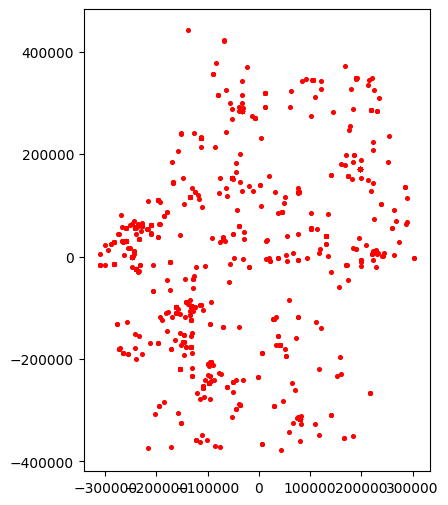
\includegraphics{labs/w02_maps_files/figure-pdf/cell-5-output-1.png}

Slightly improving the plot:

\begin{Shaded}
\begin{Highlighting}[]
\CommentTok{\# removing ticks}
\NormalTok{ax.xaxis.set\_ticklabels([])}
\NormalTok{ax.yaxis.set\_ticklabels([])}
\NormalTok{ax.tick\_params(axis}\OperatorTok{=} \StringTok{\textquotesingle{}both\textquotesingle{}}\NormalTok{, which}\OperatorTok{=} \StringTok{\textquotesingle{}both\textquotesingle{}}\NormalTok{, length}\OperatorTok{=}\DecValTok{0}\NormalTok{)}
\NormalTok{title\_parameters }\OperatorTok{=}\NormalTok{ \{}\StringTok{\textquotesingle{}fontsize\textquotesingle{}}\NormalTok{:}\StringTok{\textquotesingle{}16\textquotesingle{}}\NormalTok{, }\StringTok{\textquotesingle{}fontname\textquotesingle{}}\NormalTok{:}\StringTok{\textquotesingle{}Times New Roman\textquotesingle{}}\NormalTok{\}}
\NormalTok{ax.set\_title(}\StringTok{"Terroristic Attacks in Germany"}\NormalTok{, }\OperatorTok{**}\NormalTok{title\_parameters)}
\NormalTok{fig}
\end{Highlighting}
\end{Shaded}

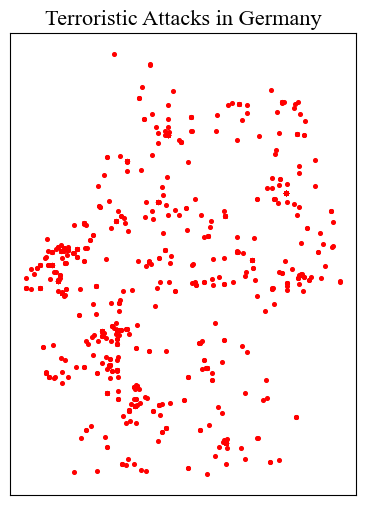
\includegraphics{labs/w02_maps_files/figure-pdf/cell-6-output-1.png}

\subsubsection{\texorpdfstring{Adding some context: Base Maps with
\texttt{Contextily}}{Adding some context: Base Maps with Contextily}}\label{adding-some-context-base-maps-with-contextily}

see providers and options here
https://xyzservices.readthedocs.io/en/stable/introduction.html

\begin{Shaded}
\begin{Highlighting}[]
\NormalTok{source }\OperatorTok{=}\NormalTok{ ctx.providers.CartoDB.Positron}
\NormalTok{ctx.add\_basemap(ax, crs}\OperatorTok{=}\NormalTok{ gdf.crs.to\_string(), source}\OperatorTok{=}\NormalTok{ source)}
\CommentTok{\# replot}
\NormalTok{fig}
\end{Highlighting}
\end{Shaded}

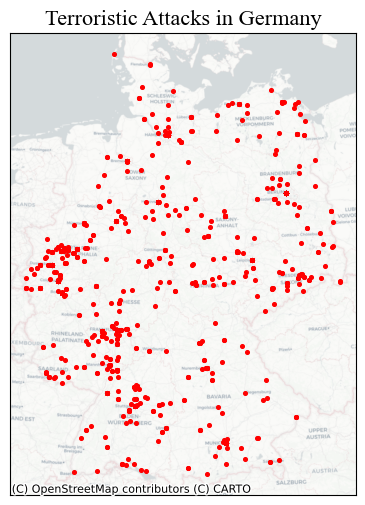
\includegraphics{labs/w02_maps_files/figure-pdf/cell-7-output-1.png}

\begin{verbatim}
<Figure size 640x480 with 0 Axes>
\end{verbatim}

\subsubsection{\texorpdfstring{Parameters specific to \texttt{Point} in
the \texttt{plot}
method}{Parameters specific to Point in the plot method}}\label{parameters-specific-to-point-in-the-plot-method}

\begin{itemize}
\tightlist
\item
  \texttt{markersize}: numerical value (for now)
\item
  \texttt{marker}: see
  https://matplotlib.org/stable/api/markers\_api.html
\end{itemize}

\paragraph{Other properties, shape
independent:}\label{other-properties-shape-independent}

\begin{itemize}
\tightlist
\item
  \texttt{color}:
  https://matplotlib.org/3.1.0/gallery/color/named\_colors.html
\item
  \texttt{alpha}: regulates transparency of the shape: 0 to 1
\end{itemize}

\begin{Shaded}
\begin{Highlighting}[]
\CommentTok{\# first, let\textquotesingle{}s make a function}

\KeywordTok{def}\NormalTok{ ax\_ticks\_off(ax):}
\NormalTok{    ax.xaxis.set\_ticklabels([])}
\NormalTok{    ax.yaxis.set\_ticklabels([])}
\NormalTok{    ax.tick\_params(axis}\OperatorTok{=} \StringTok{\textquotesingle{}both\textquotesingle{}}\NormalTok{, which}\OperatorTok{=} \StringTok{\textquotesingle{}both\textquotesingle{}}\NormalTok{, length}\OperatorTok{=}\DecValTok{0}\NormalTok{)}
\end{Highlighting}
\end{Shaded}

\begin{Shaded}
\begin{Highlighting}[]
\CommentTok{\# prepare the axis and coordinate}
\NormalTok{fig, ax }\OperatorTok{=}\NormalTok{ plt.subplots(}\DecValTok{1}\NormalTok{, }\DecValTok{1}\NormalTok{, figsize}\OperatorTok{=}\NormalTok{(}\DecValTok{8}\NormalTok{, }\DecValTok{6}\NormalTok{))}
\NormalTok{gdf.plot(ax}\OperatorTok{=}\NormalTok{ax, markersize }\OperatorTok{=} \DecValTok{15}\NormalTok{, color }\OperatorTok{=} \StringTok{\textquotesingle{}blue\textquotesingle{}}\NormalTok{, marker }\OperatorTok{=} \StringTok{\textquotesingle{}*\textquotesingle{}}\NormalTok{, alpha }\OperatorTok{=} \FloatTok{0.3}\NormalTok{)}
\NormalTok{ctx.add\_basemap(ax, crs}\OperatorTok{=}\NormalTok{ gdf.crs.to\_string(), source}\OperatorTok{=}\NormalTok{ source)}
\NormalTok{ax\_ticks\_off(ax)}
\end{Highlighting}
\end{Shaded}

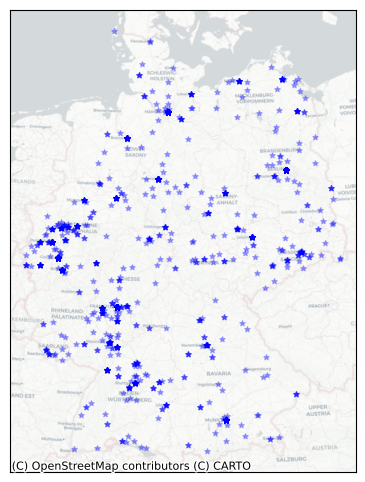
\includegraphics{labs/w02_maps_files/figure-pdf/cell-9-output-1.png}

\subsection{Plotting LineStrings}\label{plotting-linestrings}

Let's import railway tracks in the Western Balkans (Slovenia, Croatia,
Bosnia \& Herzegovina, Montenegro, Serbia, Kosovo)

\begin{Shaded}
\begin{Highlighting}[]
\NormalTok{wb\_crs }\OperatorTok{=} \StringTok{\textquotesingle{}EPSG:31277\textquotesingle{}}
\NormalTok{lines\_gdf }\OperatorTok{=}\NormalTok{ gpd.read\_file(}\StringTok{"..\textbackslash{}data\textbackslash{}wb\_railways.shp"}\NormalTok{)}
\NormalTok{lines\_gdf.plot()}
\end{Highlighting}
\end{Shaded}

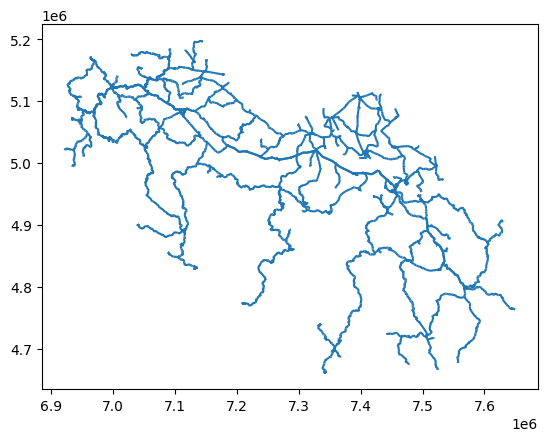
\includegraphics{labs/w02_maps_files/figure-pdf/cell-10-output-1.png}

\begin{Shaded}
\begin{Highlighting}[]
\CommentTok{\# prepare the plot}
\NormalTok{fig, ax }\OperatorTok{=}\NormalTok{ plt.subplots(}\DecValTok{1}\NormalTok{, }\DecValTok{1}\NormalTok{, figsize}\OperatorTok{=}\NormalTok{(}\DecValTok{8}\NormalTok{, }\DecValTok{6}\NormalTok{))}
\NormalTok{lines\_gdf.plot(ax}\OperatorTok{=}\NormalTok{ax, linewidth }\OperatorTok{=} \FloatTok{0.8}\NormalTok{, color }\OperatorTok{=} \StringTok{\textquotesingle{}blue\textquotesingle{}}\NormalTok{, alpha }\OperatorTok{=} \DecValTok{1}\NormalTok{)}
\NormalTok{ctx.add\_basemap(ax, crs}\OperatorTok{=}\NormalTok{ lines\_gdf.crs.to\_string(), source }\OperatorTok{=}\NormalTok{ ctx.providers.Esri.WorldGrayCanvas)}
\NormalTok{ax\_ticks\_off(ax)}
\NormalTok{ax.set\_title(}\StringTok{"Railway infrastructure in the West Balkans"}\NormalTok{, }\OperatorTok{**}\NormalTok{title\_parameters) }\CommentTok{\#parameters as above}
\end{Highlighting}
\end{Shaded}

\begin{verbatim}
Text(0.5, 1.0, 'Railway infrastructure in the West Balkans')
\end{verbatim}

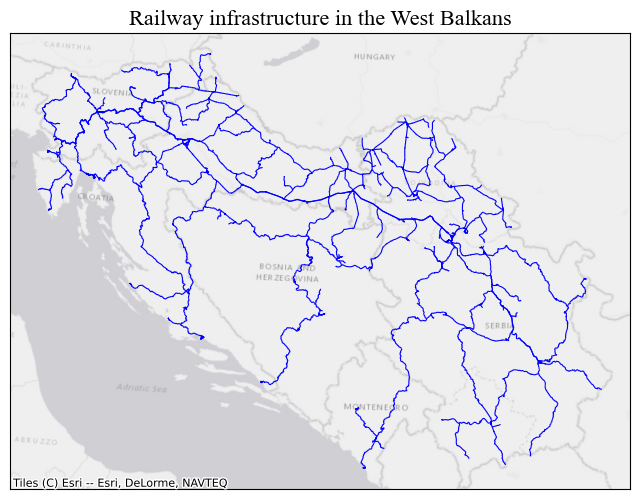
\includegraphics{labs/w02_maps_files/figure-pdf/cell-11-output-2.png}

One can also filter prior to plotting, based on the columns in the
GeoDataFrame. First we download Serbia's Boundary with \texttt{OSMNX},
more on that later on. Then we filter \texttt{lines\_gdf} with a
\texttt{within} operation.

\begin{Shaded}
\begin{Highlighting}[]
\NormalTok{serbia }\OperatorTok{=}\NormalTok{ ox.geocode\_to\_gdf(}\StringTok{\textquotesingle{}Serbia\textquotesingle{}}\NormalTok{)}
\NormalTok{serbia }\OperatorTok{=}\NormalTok{ serbia.to\_crs(wb\_crs)}
\NormalTok{serbia\_lines }\OperatorTok{=}\NormalTok{ lines\_gdf[lines\_gdf.geometry.within(serbia.iloc[}\DecValTok{0}\NormalTok{].geometry)].copy() }\CommentTok{\#there\textquotesingle{}s only one polygon in the gdf}
\end{Highlighting}
\end{Shaded}

\begin{Shaded}
\begin{Highlighting}[]
\CommentTok{\# prepare the plot}
\NormalTok{fig, ax }\OperatorTok{=}\NormalTok{ plt.subplots(}\DecValTok{1}\NormalTok{, }\DecValTok{1}\NormalTok{, figsize}\OperatorTok{=}\NormalTok{(}\DecValTok{8}\NormalTok{, }\DecValTok{6}\NormalTok{))}
\NormalTok{serbia\_lines.plot(ax}\OperatorTok{=}\NormalTok{ax, linewidth }\OperatorTok{=} \FloatTok{0.8}\NormalTok{, color }\OperatorTok{=} \StringTok{\textquotesingle{}blue\textquotesingle{}}\NormalTok{, alpha }\OperatorTok{=} \DecValTok{1}\NormalTok{)}
\NormalTok{ctx.add\_basemap(ax, crs}\OperatorTok{=}\NormalTok{ lines\_gdf.crs.to\_string(), source }\OperatorTok{=}\NormalTok{ ctx.providers.Esri.WorldGrayCanvas)}
\NormalTok{ax\_ticks\_off(ax)}
\NormalTok{ax.set\_title(}\StringTok{"Railway infrastructure in Serbia and Kosovo"}\NormalTok{, }\OperatorTok{**}\NormalTok{title\_parameters) }\CommentTok{\#parameters as above}
\end{Highlighting}
\end{Shaded}

\begin{verbatim}
Text(0.5, 1.0, 'Railway infrastructure in Serbia and Kosovo')
\end{verbatim}

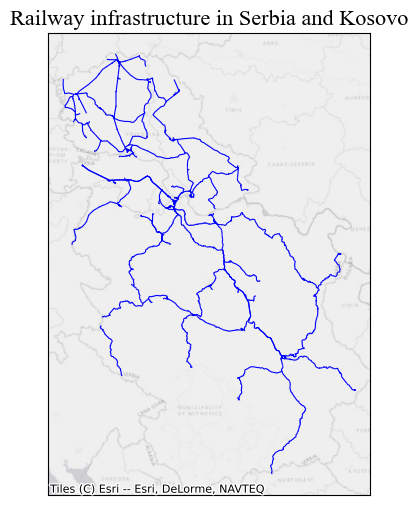
\includegraphics{labs/w02_maps_files/figure-pdf/cell-13-output-2.png}

\subsubsection{\texorpdfstring{Parameters specific to
\texttt{LineString}:}{Parameters specific to LineString:}}\label{parameters-specific-to-linestring}

\begin{itemize}
\tightlist
\item
  \texttt{linewidth}: numerical value (for now).
\item
  \texttt{capstyle}: controls how Matplotlib draws the corners where two
  different line segments meet. See
  https://matplotlib.org/stable/gallery/lines\_bars\_and\_markers/capstyle.html
\item
  \texttt{joinstyle}': controls how Matplotlib draws the corners where
  two different line segments meet.
  https://matplotlib.org/stable/gallery/lines\_bars\_and\_markers/joinstyle.html
\end{itemize}

\begin{Shaded}
\begin{Highlighting}[]
\CommentTok{\# prepare the plot}
\NormalTok{fig, ax }\OperatorTok{=}\NormalTok{ plt.subplots(}\DecValTok{1}\NormalTok{, }\DecValTok{1}\NormalTok{, figsize}\OperatorTok{=}\NormalTok{(}\DecValTok{10}\NormalTok{, }\DecValTok{10}\NormalTok{))}
\NormalTok{serbia\_lines.plot(ax}\OperatorTok{=}\NormalTok{ax, linewidth }\OperatorTok{=} \FloatTok{0.9}\NormalTok{, color }\OperatorTok{=} \StringTok{\textquotesingle{}black\textquotesingle{}}\NormalTok{, alpha }\OperatorTok{=} \DecValTok{1}\NormalTok{, capstyle }\OperatorTok{=} \StringTok{\textquotesingle{}round\textquotesingle{}}\NormalTok{, joinstyle }\OperatorTok{=} \StringTok{\textquotesingle{}round\textquotesingle{}}\NormalTok{)}
\NormalTok{ax.set\_axis\_off() }\CommentTok{\# we don\textquotesingle{}t need the ticks function}
\NormalTok{ax.set\_title(}\StringTok{"Railway infrastructure in Serbia"}\NormalTok{, }\OperatorTok{**}\NormalTok{title\_parameters) }\CommentTok{\#parameters as above}
\end{Highlighting}
\end{Shaded}

\begin{verbatim}
Text(0.5, 1.0, 'Railway infrastructure in Serbia')
\end{verbatim}

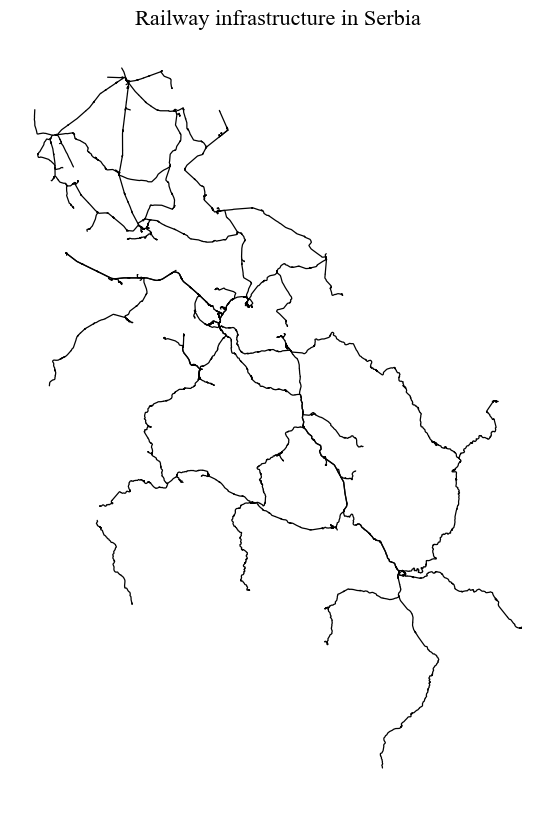
\includegraphics{labs/w02_maps_files/figure-pdf/cell-14-output-2.png}

\subsection{Plotting Polygons}\label{plotting-polygons}

We are again using \texttt{OSMNX} to download data from
\texttt{OpenStreetMap} automatically. In this case, we will get building
footprints from the city of Algiers in Alageria.

\subsubsection{\texorpdfstring{Parameter specific to
\texttt{Polygon}:}{Parameter specific to Polygon:}}\label{parameter-specific-to-polygon}

\begin{itemize}
\tightlist
\item
  \texttt{edgecolor}: the outline of the polygon, by default =
  \texttt{None} (often better).
\item
  \texttt{linewidth}: the width of the outline of the polygon.
\end{itemize}

\begin{Shaded}
\begin{Highlighting}[]
\NormalTok{algeria\_crs }\OperatorTok{=} \StringTok{\textquotesingle{}EPSG:30729\textquotesingle{}}
\NormalTok{tags }\OperatorTok{=}\NormalTok{ \{}\StringTok{"building"}\NormalTok{: }\VariableTok{True}\NormalTok{\} }\CommentTok{\#OSM tags}
\NormalTok{buildings }\OperatorTok{=}\NormalTok{ ox.features\_from\_address(}\StringTok{"Algiers, Algeria"}\NormalTok{, tags }\OperatorTok{=}\NormalTok{ tags, dist }\OperatorTok{=} \DecValTok{2000}\NormalTok{) }
\NormalTok{buildings }\OperatorTok{=}\NormalTok{ buildings.reset\_index()}
 \CommentTok{\# sometimes building footprints are represented by Points, let\textquotesingle{}s disregard them}
\NormalTok{buildings }\OperatorTok{=}\NormalTok{ buildings[(buildings.geometry.geom\_type }\OperatorTok{==} \StringTok{\textquotesingle{}Polygon\textquotesingle{}}\NormalTok{) }\OperatorTok{|}\NormalTok{ (buildings.geometry.geom\_type }\OperatorTok{==} \StringTok{\textquotesingle{}MultiPolygon\textquotesingle{}}\NormalTok{)]}
\NormalTok{buildings }\OperatorTok{=}\NormalTok{ buildings.to\_crs(algeria\_crs)}
\end{Highlighting}
\end{Shaded}

\begin{Shaded}
\begin{Highlighting}[]
\NormalTok{fig, ax }\OperatorTok{=}\NormalTok{ plt.subplots(}\DecValTok{1}\NormalTok{, }\DecValTok{1}\NormalTok{, figsize}\OperatorTok{=}\NormalTok{(}\DecValTok{15}\NormalTok{, }\DecValTok{10}\NormalTok{))}
\NormalTok{ax.set\_title(}\StringTok{"Buildings in Algiers"}\NormalTok{, }\OperatorTok{**}\NormalTok{title\_parameters)}
\NormalTok{ax.set\_axis\_off() }\CommentTok{\# we don\textquotesingle{}t need the ticks function}
\NormalTok{buildings.plot(ax}\OperatorTok{=}\NormalTok{ax, color }\OperatorTok{=} \StringTok{\textquotesingle{}orange\textquotesingle{}}\NormalTok{, edgecolor }\OperatorTok{=} \StringTok{\textquotesingle{}black\textquotesingle{}}\NormalTok{, lw }\OperatorTok{=} \FloatTok{0.2}\NormalTok{)}
\NormalTok{source }\OperatorTok{=}\NormalTok{ ctx.providers.CartoDB.PositronNoLabels}
\NormalTok{ctx.add\_basemap(ax, crs}\OperatorTok{=}\NormalTok{ buildings.crs.to\_string(), source}\OperatorTok{=}\NormalTok{ source)}
\end{Highlighting}
\end{Shaded}

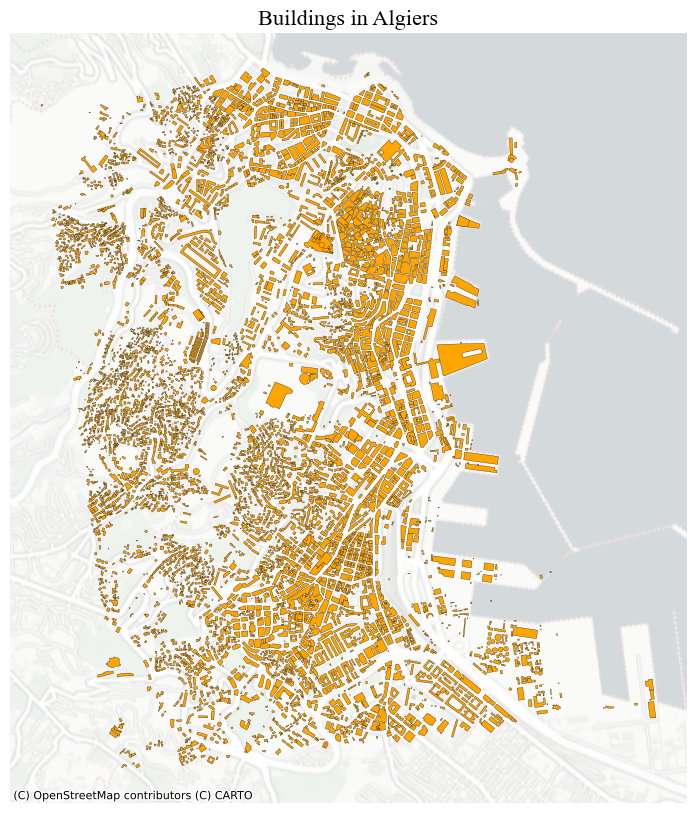
\includegraphics{labs/w02_maps_files/figure-pdf/cell-16-output-1.png}

For polygons, you can also plot just the boundaries of the geometries
by:

\begin{Shaded}
\begin{Highlighting}[]
\NormalTok{buildings.boundary.plot(lw }\OperatorTok{=} \FloatTok{0.5}\NormalTok{)}
\end{Highlighting}
\end{Shaded}

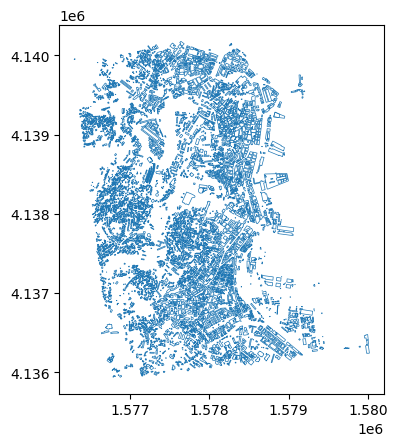
\includegraphics{labs/w02_maps_files/figure-pdf/cell-17-output-1.png}

\subsection{Plotting more than one layer
together}\label{plotting-more-than-one-layer-together}

Let's also download roads for Algiers

\begin{Shaded}
\begin{Highlighting}[]
\NormalTok{tags }\OperatorTok{=}\NormalTok{ \{}\StringTok{"highway"}\NormalTok{: }\VariableTok{True}\NormalTok{\} }\CommentTok{\#OSM tags}
\NormalTok{roads }\OperatorTok{=}\NormalTok{ ox.features\_from\_address(}\StringTok{"Algiers, Algeria"}\NormalTok{, tags }\OperatorTok{=}\NormalTok{ tags, dist }\OperatorTok{=} \DecValTok{2000}\NormalTok{) }
\NormalTok{roads }\OperatorTok{=}\NormalTok{ roads.reset\_index()}
\NormalTok{roads }\OperatorTok{=}\NormalTok{ roads.to\_crs(algeria\_crs)}
 \CommentTok{\# sometimes building footprints are represented by Points, let\textquotesingle{}s disregard them}
\NormalTok{roads }\OperatorTok{=}\NormalTok{ roads[roads.geometry.geom\_type }\OperatorTok{==} \StringTok{\textquotesingle{}LineString\textquotesingle{}}\NormalTok{]}
\end{Highlighting}
\end{Shaded}

And plot everything togehter. It's important to keep in mind that the
last layer is always rendered on top of the others. In other words, they
may cover the previous ones.

However, you can prevent this by passing arguments to the parameter
\texttt{zorder} in the \texttt{plot} method. The layer with the higher
zorder value will be plotted on top.

\begin{Shaded}
\begin{Highlighting}[]
\NormalTok{fig, ax }\OperatorTok{=}\NormalTok{ plt.subplots(}\DecValTok{1}\NormalTok{, }\DecValTok{1}\NormalTok{, figsize}\OperatorTok{=}\NormalTok{(}\DecValTok{15}\NormalTok{, }\DecValTok{10}\NormalTok{))}
\NormalTok{ax.set\_title(}\StringTok{"Buildings and Roads in Algiers"}\NormalTok{, }\OperatorTok{**}\NormalTok{title\_parameters)}
\NormalTok{ax.set\_axis\_off() }\CommentTok{\# we don\textquotesingle{}t need the ticks function}
\CommentTok{\# only roads within the extent of the buildings layer}
\NormalTok{roads[roads.geometry.within(buildings.unary\_union.envelope)].plot(ax}\OperatorTok{=}\NormalTok{ax, color }\OperatorTok{=} \StringTok{\textquotesingle{}grey\textquotesingle{}}\NormalTok{, lw }\OperatorTok{=} \FloatTok{0.5}\NormalTok{) }\CommentTok{\#linewidth can be also passed as lw }
\NormalTok{buildings.plot(ax}\OperatorTok{=}\NormalTok{ax, color }\OperatorTok{=} \StringTok{\textquotesingle{}orange\textquotesingle{}}\NormalTok{)}
\end{Highlighting}
\end{Shaded}

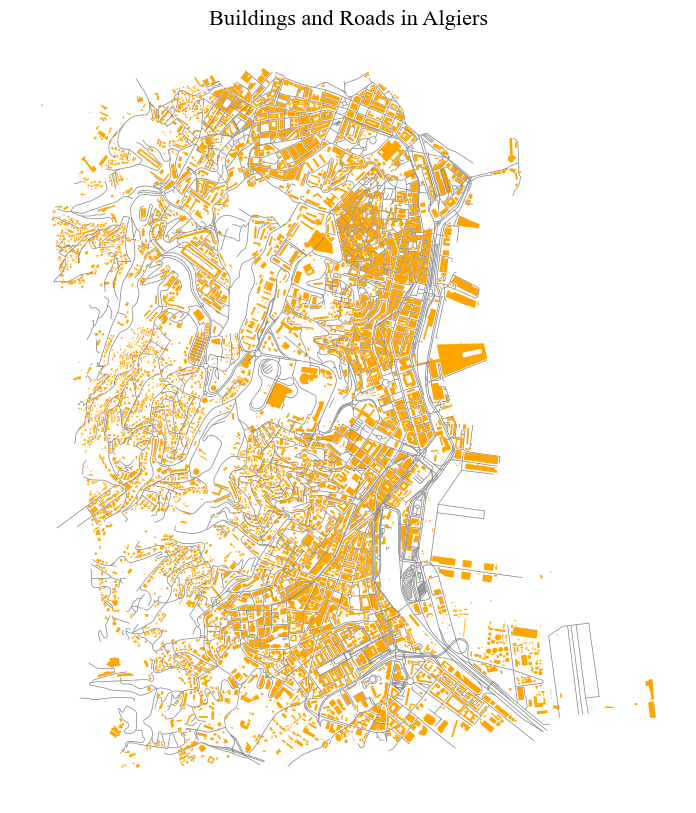
\includegraphics{labs/w02_maps_files/figure-pdf/cell-19-output-1.png}

\subsection{Sub-plots}\label{sub-plots}

To obtain multiple sub-plots, we manipulate the \texttt{nrows},
\texttt{ncols} parameters. We can use this approach to: * Plot the same
layer with different properties.

\begin{Shaded}
\begin{Highlighting}[]
\NormalTok{fig, axes }\OperatorTok{=}\NormalTok{ plt.subplots(}\DecValTok{1}\NormalTok{, }\DecValTok{2}\NormalTok{, figsize}\OperatorTok{=}\NormalTok{(}\DecValTok{10}\NormalTok{, }\DecValTok{6}\NormalTok{))}
\NormalTok{colors }\OperatorTok{=}\NormalTok{ [}\StringTok{\textquotesingle{}red\textquotesingle{}}\NormalTok{, }\StringTok{\textquotesingle{}blue\textquotesingle{}}\NormalTok{]}

\ControlFlowTok{for}\NormalTok{ n, ax }\KeywordTok{in} \BuiltInTok{enumerate}\NormalTok{(axes):}
\NormalTok{    gdf.plot(ax}\OperatorTok{=}\NormalTok{ax, markersize }\OperatorTok{=} \DecValTok{4}\NormalTok{, color }\OperatorTok{=}\NormalTok{ colors[n])}
\NormalTok{    ax.set\_axis\_off()}
\NormalTok{    ctx.add\_basemap(ax, crs}\OperatorTok{=}\NormalTok{ gdf.crs.to\_string(), source}\OperatorTok{=}\NormalTok{ source)}
\end{Highlighting}
\end{Shaded}

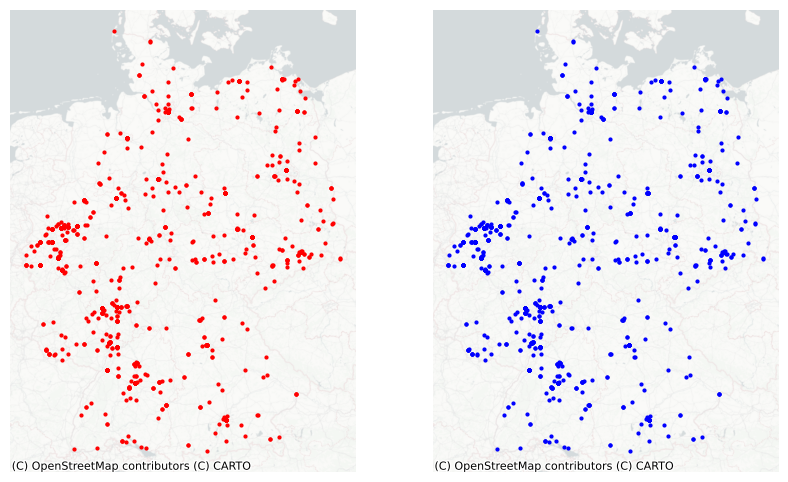
\includegraphics{labs/w02_maps_files/figure-pdf/cell-20-output-1.png}

\begin{itemize}
\tightlist
\item
  Plot different layers.
\end{itemize}

\begin{Shaded}
\begin{Highlighting}[]
\NormalTok{fig, axes }\OperatorTok{=}\NormalTok{ plt.subplots(}\DecValTok{1}\NormalTok{, }\DecValTok{2}\NormalTok{, figsize}\OperatorTok{=}\NormalTok{(}\DecValTok{10}\NormalTok{, }\DecValTok{6}\NormalTok{))}
\NormalTok{gdfs }\OperatorTok{=}\NormalTok{ [buildings, roads]}
\NormalTok{colors }\OperatorTok{=}\NormalTok{ [}\StringTok{\textquotesingle{}orange\textquotesingle{}}\NormalTok{, }\StringTok{\textquotesingle{}grey\textquotesingle{}}\NormalTok{]}

\NormalTok{buildings.plot(ax}\OperatorTok{=}\NormalTok{axes[}\DecValTok{0}\NormalTok{], color }\OperatorTok{=} \StringTok{\textquotesingle{}orange\textquotesingle{}}\NormalTok{, edgecolor }\OperatorTok{=} \StringTok{\textquotesingle{}none\textquotesingle{}}\NormalTok{)}
\NormalTok{roads.plot(ax}\OperatorTok{=}\NormalTok{axes[}\DecValTok{1}\NormalTok{], color }\OperatorTok{=} \StringTok{\textquotesingle{}gray\textquotesingle{}}\NormalTok{, lw }\OperatorTok{=} \FloatTok{0.5}\NormalTok{)}

\ControlFlowTok{for}\NormalTok{ ax }\KeywordTok{in}\NormalTok{ axes:}
\NormalTok{    ax.set\_axis\_off()}
\NormalTok{    ctx.add\_basemap(ax, crs}\OperatorTok{=}\NormalTok{ buildings.crs.to\_string(), source }\OperatorTok{=}\NormalTok{ source)}
\end{Highlighting}
\end{Shaded}

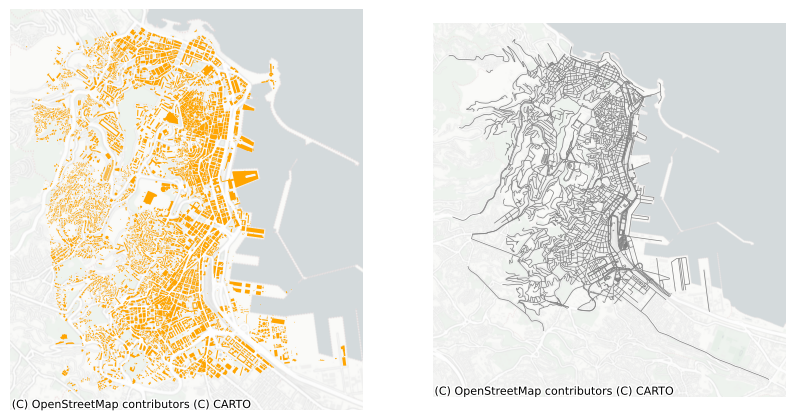
\includegraphics{labs/w02_maps_files/figure-pdf/cell-21-output-1.png}

\begin{itemize}
\tightlist
\item
  Analyse phenomena across different geographical areas. For example,
  terrorism in Germany and in the UK.
\end{itemize}

\begin{Shaded}
\begin{Highlighting}[]
\CommentTok{\# let\textquotesingle{}s prepare the gdf for the UK}
\NormalTok{df\_uk }\OperatorTok{=}\NormalTok{ attacks[attacks.country\_txt }\OperatorTok{==} \StringTok{\textquotesingle{}United Kingdom\textquotesingle{}}\NormalTok{].copy()}
\NormalTok{uk\_crs }\OperatorTok{=} \StringTok{\textquotesingle{}EPSG:27700\textquotesingle{}}
\NormalTok{gdf\_uk }\OperatorTok{=}\NormalTok{ gpd.GeoDataFrame(df\_uk, geometry}\OperatorTok{=}\NormalTok{gpd.points\_from\_xy(df\_uk.longitude, df\_uk.latitude), crs }\OperatorTok{=}\NormalTok{ wgs)}
\NormalTok{gdf\_uk }\OperatorTok{=}\NormalTok{ gdf\_uk.to\_crs(uk\_crs)}
\end{Highlighting}
\end{Shaded}

\begin{Shaded}
\begin{Highlighting}[]
\NormalTok{fig, axes }\OperatorTok{=}\NormalTok{ plt.subplots(}\DecValTok{1}\NormalTok{, }\DecValTok{2}\NormalTok{, figsize}\OperatorTok{=}\NormalTok{(}\DecValTok{10}\NormalTok{, }\DecValTok{6}\NormalTok{))}
\NormalTok{gdfs }\OperatorTok{=}\NormalTok{ [gdf, gdf\_uk]}

\ControlFlowTok{for}\NormalTok{ n, ax }\KeywordTok{in} \BuiltInTok{enumerate}\NormalTok{(axes):}
\NormalTok{    gdf\_tmp }\OperatorTok{=}\NormalTok{ gdfs[n]}
\NormalTok{    gdf\_tmp.plot(ax}\OperatorTok{=}\NormalTok{ax, color }\OperatorTok{=} \StringTok{\textquotesingle{}orange\textquotesingle{}}\NormalTok{, markersize }\OperatorTok{=} \DecValTok{3}\NormalTok{)}
\NormalTok{    ax.set\_axis\_off()}
\NormalTok{    ctx.add\_basemap(ax, crs}\OperatorTok{=}\NormalTok{ gdf\_tmp.crs.to\_string(), source}\OperatorTok{=}\NormalTok{ source)}
\end{Highlighting}
\end{Shaded}

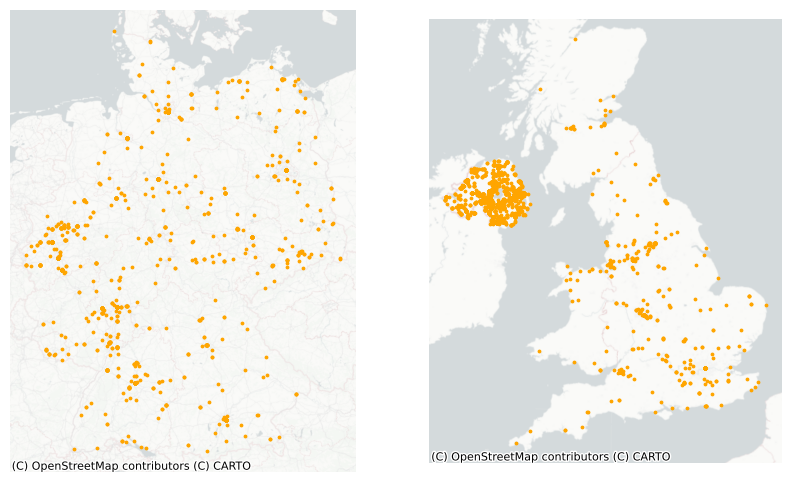
\includegraphics{labs/w02_maps_files/figure-pdf/cell-23-output-1.png}

\textbf{Exercise}:

\begin{itemize}
\tightlist
\item
  Think about the plots above and how they could be improved.
\item
  Copy and paste the code and execute the functions playing with the
  different parameters.
\item
  Produce a neat map using the \texttt{GeoDataFrame}s available in this
  notebook or the ones employed in the previous sessions, making use of
  the elements/parameters discussed here.
\item
  Try out different tiles for the basemap to familiarise yourself with
  what's available.
\end{itemize}

\section{Part II: Choropleth Mapping}\label{part-ii-choropleth-mapping}

\begin{Shaded}
\begin{Highlighting}[]
\ImportTok{import}\NormalTok{ geoplot.crs }\ImportTok{as}\NormalTok{ gcrs}
\ImportTok{import}\NormalTok{ geoplot }\ImportTok{as}\NormalTok{ gplt}
\end{Highlighting}
\end{Shaded}

\textbf{Data}

For this second part of the tutorial, we will use some data at the
municipality level for Serbia. The data contains information regarding
poverty level, average income, population and tourism. The data is taken
from https://data.stat.gov.rs/?caller=SDDB\&languageCode=en-US and can
be associated to the polygons representing the administrative boundaries
of the municipalities. These boundaries can be found here
https://data.humdata.org/dataset/geoboundaries-admin-boundaries-for-serbia?force\_layout=desktop.
While most of the data refers to 2023, the admin boundaries file traces
back to 2017. Thus, it may contain obsolete information (few changes may
occur).

Later on, we will go back to the terrorism dataset.

\begin{Shaded}
\begin{Highlighting}[]
\CommentTok{\# This will be different on your computer and will depend on where}
\CommentTok{\# you have downloaded the files}
\NormalTok{serbia\_crs }\OperatorTok{=} \StringTok{\textquotesingle{}EPSG:31277\textquotesingle{}}
\NormalTok{wgs }\OperatorTok{=} \StringTok{\textquotesingle{}EPSG:4326\textquotesingle{}}
\NormalTok{serbia\_admin }\OperatorTok{=}\NormalTok{ gpd.read\_file(}\StringTok{\textquotesingle{}../data/serbia\_admin.shp\textquotesingle{}}\NormalTok{)}
\NormalTok{serbia\_admin.set\_index(}\StringTok{\textquotesingle{}townID\textquotesingle{}}\NormalTok{, inplace }\OperatorTok{=} \VariableTok{True}\NormalTok{, drop }\OperatorTok{=} \VariableTok{True}\NormalTok{)}
\NormalTok{serbia\_admin }\OperatorTok{=}\NormalTok{ serbia\_admin.to\_crs(serbia\_crs)}
\end{Highlighting}
\end{Shaded}

Let's plot the \texttt{GeoDataFrame} following the last session's steps.

\begin{Shaded}
\begin{Highlighting}[]
\NormalTok{fig, ax }\OperatorTok{=}\NormalTok{ plt.subplots(}\DecValTok{1}\NormalTok{, }\DecValTok{1}\NormalTok{, figsize}\OperatorTok{=}\NormalTok{(}\DecValTok{8}\NormalTok{, }\DecValTok{6}\NormalTok{))}
\NormalTok{serbia\_admin.plot(ax }\OperatorTok{=}\NormalTok{ ax, color }\OperatorTok{=} \StringTok{\textquotesingle{}salmon\textquotesingle{}}\NormalTok{, linewidth }\OperatorTok{=} \FloatTok{0.3}\NormalTok{, edgecolor }\OperatorTok{=} \StringTok{\textquotesingle{}white\textquotesingle{}}\NormalTok{)}
\NormalTok{ax.set\_axis\_off()}
\NormalTok{title\_parameters }\OperatorTok{=}\NormalTok{ \{}\StringTok{\textquotesingle{}fontsize\textquotesingle{}}\NormalTok{:}\StringTok{\textquotesingle{}16\textquotesingle{}}\NormalTok{, }\StringTok{\textquotesingle{}fontname\textquotesingle{}}\NormalTok{:}\StringTok{\textquotesingle{}Times New Roman\textquotesingle{}}\NormalTok{\}}
\NormalTok{ax.set\_title(}\StringTok{"Serbian Municipalities"}\NormalTok{, }\OperatorTok{**}\NormalTok{title\_parameters) }\CommentTok{\#parameters as above}
\end{Highlighting}
\end{Shaded}

\begin{verbatim}
Text(0.5, 1.0, 'Serbian Municipalities')
\end{verbatim}

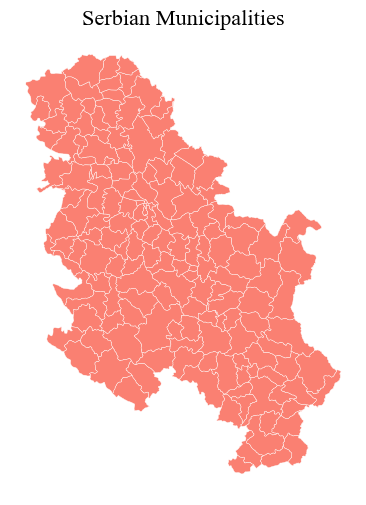
\includegraphics{labs/w02_maps_files/figure-pdf/cell-26-output-2.png}

The we load the data and merge it into the \texttt{GeoDataFrame}, before
getting rid of municipalities that do not have a corresponding
shape/record in the GeoDataFrame (probably the result of changes in the
national subdivisions).

\begin{Shaded}
\begin{Highlighting}[]
\NormalTok{data }\OperatorTok{=}\NormalTok{ pd.read\_csv(}\StringTok{"../data/serbia\_data.csv"}\NormalTok{) }\CommentTok{\#some slavic characters }
\NormalTok{data.drop(}\StringTok{\textquotesingle{}name\_en\textquotesingle{}}\NormalTok{, axis }\OperatorTok{=} \DecValTok{1}\NormalTok{, inplace }\OperatorTok{=} \VariableTok{True}\NormalTok{)}
\NormalTok{serbia\_admin }\OperatorTok{=}\NormalTok{ pd.merge(serbia\_admin, data, left\_on }\OperatorTok{=} \StringTok{"townID"}\NormalTok{, right\_on }\OperatorTok{=} \StringTok{"id"}\NormalTok{)}
\NormalTok{serbia\_admin }\OperatorTok{=}\NormalTok{ serbia\_admin[serbia\_admin.}\BuiltInTok{id}\NormalTok{.notna()]}
\NormalTok{serbia\_admin[}\StringTok{\textquotesingle{}id\textquotesingle{}}\NormalTok{] }\OperatorTok{=}\NormalTok{ serbia\_admin[}\StringTok{\textquotesingle{}id\textquotesingle{}}\NormalTok{].astype(}\StringTok{\textquotesingle{}int64\textquotesingle{}}\NormalTok{)}
\NormalTok{serbia\_admin.head()}

\CommentTok{\#let\textquotesingle{}s save the so{-}obtained gdf for later (encoding for dealing with slavic characters).}
\NormalTok{serbia\_admin.to\_file(}\StringTok{"../data/serbia\_data.shp"}\NormalTok{, encoding}\OperatorTok{=}\StringTok{\textquotesingle{}utf{-}8\textquotesingle{}}\NormalTok{)}
\end{Highlighting}
\end{Shaded}

Creating a choropleth map is rather straightforward and can ben done by
using few other parameters. Reflect on what you see and whether the map
below is informative.

\begin{Shaded}
\begin{Highlighting}[]
\NormalTok{fig, ax }\OperatorTok{=}\NormalTok{ plt.subplots(}\DecValTok{1}\NormalTok{, }\DecValTok{1}\NormalTok{, figsize}\OperatorTok{=}\NormalTok{(}\DecValTok{8}\NormalTok{, }\DecValTok{6}\NormalTok{))}
\NormalTok{serbia\_admin.plot(ax }\OperatorTok{=}\NormalTok{ ax, column }\OperatorTok{=} \StringTok{\textquotesingle{}gross\textquotesingle{}}\NormalTok{, linewidth }\OperatorTok{=} \FloatTok{0.3}\NormalTok{, cmap }\OperatorTok{=} \StringTok{\textquotesingle{}Greens\textquotesingle{}}\NormalTok{, legend }\OperatorTok{=} \VariableTok{True}\NormalTok{)}
\NormalTok{ax.set\_axis\_off()}
\NormalTok{title\_parameters }\OperatorTok{=}\NormalTok{ \{}\StringTok{\textquotesingle{}fontsize\textquotesingle{}}\NormalTok{:}\StringTok{\textquotesingle{}16\textquotesingle{}}\NormalTok{, }\StringTok{\textquotesingle{}fontname\textquotesingle{}}\NormalTok{:}\StringTok{\textquotesingle{}Times New Roman\textquotesingle{}}\NormalTok{\}}
\NormalTok{ax.set\_title(}\StringTok{"Serbian Municipalities"}\NormalTok{, }\OperatorTok{**}\NormalTok{title\_parameters) }\CommentTok{\#parameters as above}
\end{Highlighting}
\end{Shaded}

\begin{verbatim}
Text(0.5, 1.0, 'Serbian Municipalities')
\end{verbatim}

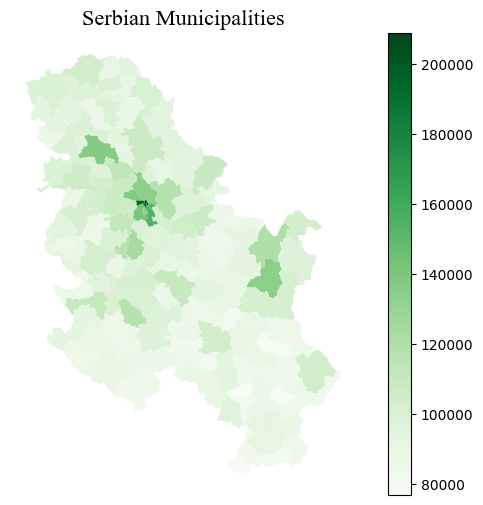
\includegraphics{labs/w02_maps_files/figure-pdf/cell-28-output-2.png}

\subsection{Choropleth Maps for Numerical
Variables}\label{choropleth-maps-for-numerical-variables}

We are essentially using the same approach employed for creating basic
maps, the method \texttt{plot}, but we now need to pass arguments to
some new parameters to specify which column is to be represented and
how. As an optional argument, one can set legend to \texttt{True} and
the resulting figure will include a colour bar.

\begin{itemize}
\tightlist
\item
  \texttt{column}: the name of the column representing the variable that
  we want to use to colour-code our shapes.
\item
  \texttt{scheme}: the scheme used to colour the shapes based on the
  variable values.
\item
  \texttt{cmap}: the colormap used to show variation.
\end{itemize}

\subsubsection{Colormaps}\label{colormaps}

Built-in colour maps can be found here
https://matplotlib.org/stable/gallery/color/colormap\_reference.html.
However one can create new ones as follows from a list of colours:

\begin{Shaded}
\begin{Highlighting}[]
\ImportTok{from}\NormalTok{ seaborn }\ImportTok{import}\NormalTok{ palplot}
\ImportTok{from}\NormalTok{ matplotlib.colors }\ImportTok{import}\NormalTok{ LinearSegmentedColormap}

\NormalTok{colors }\OperatorTok{=}\NormalTok{ [(}\FloatTok{0.00}\NormalTok{, }\FloatTok{0.00}\NormalTok{, }\FloatTok{0.00}\NormalTok{,}\DecValTok{1}\NormalTok{), (}\FloatTok{0.248}\NormalTok{, }\FloatTok{0.0271}\NormalTok{, }\FloatTok{0.569}\NormalTok{, }\DecValTok{1}\NormalTok{), (}\FloatTok{0.0311}\NormalTok{, }\FloatTok{0.258}\NormalTok{, }\FloatTok{0.646}\NormalTok{,}\DecValTok{1}\NormalTok{),}
\NormalTok{            (}\FloatTok{0.019}\NormalTok{, }\FloatTok{0.415}\NormalTok{, }\FloatTok{0.415}\NormalTok{,}\DecValTok{1}\NormalTok{), (}\FloatTok{0.025}\NormalTok{, }\FloatTok{0.538}\NormalTok{, }\FloatTok{0.269}\NormalTok{,}\DecValTok{1}\NormalTok{), (}\FloatTok{0.0315}\NormalTok{, }\FloatTok{0.658}\NormalTok{, }\FloatTok{0.103}\NormalTok{,}\DecValTok{1}\NormalTok{),}
\NormalTok{            (}\FloatTok{0.331}\NormalTok{, }\FloatTok{0.761}\NormalTok{, }\FloatTok{0.036}\NormalTok{,}\DecValTok{1}\NormalTok{),(}\FloatTok{0.768}\NormalTok{, }\FloatTok{0.809}\NormalTok{, }\FloatTok{0.039}\NormalTok{,}\DecValTok{1}\NormalTok{), (}\FloatTok{0.989}\NormalTok{, }\FloatTok{0.862}\NormalTok{, }\FloatTok{0.772}\NormalTok{,}\DecValTok{1}\NormalTok{),}
\NormalTok{            (}\FloatTok{1.0}\NormalTok{, }\FloatTok{1.0}\NormalTok{, }\FloatTok{1.0}\NormalTok{)]}
\NormalTok{palplot(colors)}
\end{Highlighting}
\end{Shaded}

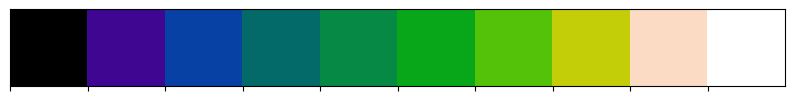
\includegraphics{labs/w02_maps_files/figure-pdf/cell-29-output-1.png}

\begin{Shaded}
\begin{Highlighting}[]
\NormalTok{kindlmann }\OperatorTok{=}\NormalTok{ LinearSegmentedColormap.from\_list(}\StringTok{\textquotesingle{}kindlmann\textquotesingle{}}\NormalTok{, colors)}
\end{Highlighting}
\end{Shaded}

or from colour names:

\begin{Shaded}
\begin{Highlighting}[]
\NormalTok{colors }\OperatorTok{=}\NormalTok{ [}\StringTok{"white"}\NormalTok{, }\StringTok{"yellow"}\NormalTok{, }\StringTok{"red"}\NormalTok{]}
\NormalTok{palplot(colors)}
\end{Highlighting}
\end{Shaded}

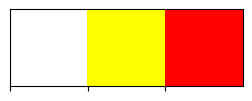
\includegraphics{labs/w02_maps_files/figure-pdf/cell-31-output-1.png}

Let's try a new colormap and let's also set a number of classes to
divide the data in, through the parameter \texttt{k}.

\begin{Shaded}
\begin{Highlighting}[]
\NormalTok{white\_to\_red }\OperatorTok{=}\NormalTok{ LinearSegmentedColormap.from\_list(}\StringTok{"name"}\NormalTok{, [}\StringTok{"yellow"}\NormalTok{,}\StringTok{"red"}\NormalTok{])}
\end{Highlighting}
\end{Shaded}

\begin{Shaded}
\begin{Highlighting}[]
\NormalTok{fig, ax }\OperatorTok{=}\NormalTok{ plt.subplots(}\DecValTok{1}\NormalTok{, }\DecValTok{1}\NormalTok{, figsize}\OperatorTok{=}\NormalTok{(}\DecValTok{8}\NormalTok{, }\DecValTok{6}\NormalTok{))}
\NormalTok{serbia\_admin.plot(ax }\OperatorTok{=}\NormalTok{ ax, column }\OperatorTok{=} \StringTok{\textquotesingle{}gross\textquotesingle{}}\NormalTok{, linewidth }\OperatorTok{=} \FloatTok{0.3}\NormalTok{, cmap }\OperatorTok{=}\NormalTok{ kindlmann.}\BuiltInTok{reversed}\NormalTok{(), legend }\OperatorTok{=} \VariableTok{True}\NormalTok{, k }\OperatorTok{=} \DecValTok{8}\NormalTok{)}
\NormalTok{ax.set\_axis\_off()}
\NormalTok{title\_parameters }\OperatorTok{=}\NormalTok{ \{}\StringTok{\textquotesingle{}fontsize\textquotesingle{}}\NormalTok{:}\StringTok{\textquotesingle{}16\textquotesingle{}}\NormalTok{, }\StringTok{\textquotesingle{}fontname\textquotesingle{}}\NormalTok{:}\StringTok{\textquotesingle{}Times New Roman\textquotesingle{}}\NormalTok{\}}
\NormalTok{ax.set\_title(}\StringTok{"Serbian Municipalities"}\NormalTok{, }\OperatorTok{**}\NormalTok{title\_parameters) }\CommentTok{\#parameters as above}
\end{Highlighting}
\end{Shaded}

\begin{verbatim}
Text(0.5, 1.0, 'Serbian Municipalities')
\end{verbatim}

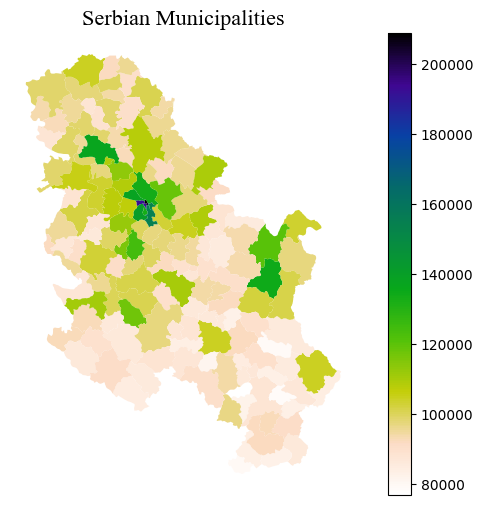
\includegraphics{labs/w02_maps_files/figure-pdf/cell-33-output-2.png}

With \texttt{GeoPandas}, when you use the \texttt{plot} method with
\texttt{legend=True} the type of legend that appears depends on the data
being visualized:

\begin{itemize}
\tightlist
\item
  Continuous Data: For columns with continuous data (like population
  estimates, temperatures, etc.), a colour bar is generated as the
  legend. This color bar represents a range of values with a gradient,
  indicating how data values correspond to colours on the map.
\item
  Categorical Data: For columns with categorical data (like country
  names, types of land use, etc.), if you specify \texttt{legend=True},
  \texttt{GeoPandas} will try to create a legend that categorizes these
  distinct values with different colours. However, creating legends for
  categorical data is not as straightforward as with continuous data and
  might require additional handling for a clear and informative legend
  (see below).
\end{itemize}

\subsubsection{Scheme}\label{scheme}

It is important to keep in mind that choropleth maps strongly depend on
the scheme that it is passed (or the default one) to classify the data
in groups. The plot above only shows one municipality coloured in dark
blue.

Look at the following plots and how three different classifiers produce
different results for the same data.

Refer to https://geopandas.org/en/stable/gallery/choropleths.html and
https://geographicdata.science/book/notebooks/05\_choropleth.html for
further details

\begin{Shaded}
\begin{Highlighting}[]
\CommentTok{\# Function for plotting the map and the distribution of the value in bins  }

\ImportTok{from}\NormalTok{ mapclassify }\ImportTok{import}\NormalTok{ Quantiles, EqualInterval, FisherJenks}

\KeywordTok{def}\NormalTok{ plot\_scheme(gdf, column, scheme, figsize}\OperatorTok{=}\NormalTok{(}\DecValTok{10}\NormalTok{, }\DecValTok{6}\NormalTok{)):}
    \CommentTok{\textquotesingle{}\textquotesingle{}\textquotesingle{}}
\CommentTok{    Arguments}
\CommentTok{    {-}{-}{-}{-}{-}{-}{-}{-}{-}}
\CommentTok{    gdf: GeoDataFrame}
\CommentTok{        The GeoDataFrame to plot}
\CommentTok{    column: str}
\CommentTok{        Variable name }
\CommentTok{    scheme: str}
\CommentTok{        Name of the classification scheme to use }
\CommentTok{    figsize: Tuple}
\CommentTok{        [Optional. Default = (10, 6)] Size of the figure to be created.}

\CommentTok{    \textquotesingle{}\textquotesingle{}\textquotesingle{}}
\NormalTok{    schemes }\OperatorTok{=}\NormalTok{ \{}\StringTok{\textquotesingle{}equal\_interval\textquotesingle{}}\NormalTok{: EqualInterval, }\StringTok{\textquotesingle{}quantiles\textquotesingle{}}\NormalTok{: Quantiles, }\StringTok{\textquotesingle{}fisher\_jenks\textquotesingle{}}\NormalTok{: FisherJenks\} }
\NormalTok{    classification }\OperatorTok{=}\NormalTok{ schemes[scheme](gdf[column], k}\OperatorTok{=}\DecValTok{7}\NormalTok{)}
\NormalTok{    fig, (ax1, ax2) }\OperatorTok{=}\NormalTok{ plt.subplots(}\DecValTok{1}\NormalTok{, }\DecValTok{2}\NormalTok{, figsize}\OperatorTok{=}\NormalTok{figsize)}
    \CommentTok{\# KDE}
\NormalTok{    sns.kdeplot(gdf[column], fill}\OperatorTok{=}\VariableTok{True}\NormalTok{, color}\OperatorTok{=}\StringTok{\textquotesingle{}purple\textquotesingle{}}\NormalTok{, ax}\OperatorTok{=}\NormalTok{ax1)}
\NormalTok{    sns.rugplot(gdf[column], alpha}\OperatorTok{=}\FloatTok{0.5}\NormalTok{, color}\OperatorTok{=}\StringTok{\textquotesingle{}purple\textquotesingle{}}\NormalTok{, ax}\OperatorTok{=}\NormalTok{ax1)}
    \ControlFlowTok{for}\NormalTok{ cut }\KeywordTok{in}\NormalTok{ classification.bins:}
\NormalTok{        ax1.axvline(cut, color}\OperatorTok{=}\StringTok{\textquotesingle{}blue\textquotesingle{}}\NormalTok{, linewidth}\OperatorTok{=}\FloatTok{0.75}\NormalTok{)}
\NormalTok{    ax1.set\_title(}\StringTok{\textquotesingle{}Value distribution\textquotesingle{}}\NormalTok{)}
    \CommentTok{\# Map}
\NormalTok{    p }\OperatorTok{=}\NormalTok{ gdf.plot(column}\OperatorTok{=}\NormalTok{column, scheme}\OperatorTok{=}\NormalTok{scheme, alpha}\OperatorTok{=}\FloatTok{0.75}\NormalTok{, k}\OperatorTok{=}\DecValTok{7}\NormalTok{, cmap}\OperatorTok{=}\StringTok{\textquotesingle{}RdPu\textquotesingle{}}\NormalTok{, ax}\OperatorTok{=}\NormalTok{ax2, linewidth}\OperatorTok{=}\FloatTok{0.1}\NormalTok{)}
\NormalTok{    ax2.axis(}\StringTok{\textquotesingle{}equal\textquotesingle{}}\NormalTok{)}
\NormalTok{    ax2.set\_axis\_off()}
\NormalTok{    ax2.set\_title(}\StringTok{\textquotesingle{}Geographical distribution\textquotesingle{}}\NormalTok{)}
\NormalTok{    fig.suptitle(scheme, size}\OperatorTok{=}\DecValTok{25}\NormalTok{)}
\NormalTok{    plt.show()}
\end{Highlighting}
\end{Shaded}

\begin{itemize}
\tightlist
\item
  The \emph{Equal intervals} method splits the range of the
  distribution, the difference between the minimum and maximum value,
  into equally large segments and to assign a different colour to each
  of them according to a palette that reflects the fact that values are
  ordered.
\item
  To obtain a more balanced classification, one can use the
  \emph{Quantiles} scheme. This assigns the same amount of values to
  each bin: the entire series is laid out in order and break points are
  assigned in a way that leaves exactly the same amount of observations
  between each of them. This ``observation-based'' approach contrasts
  with the ``value-based'' method of equal intervals and, although it
  can obscure the magnitude of extreme values, it can be more
  informative in cases with skewed distributions.
\item
  Amongst many other, the \emph{Fisher Jenks} dynamically minimises the
  sum of the absolute deviations around class medians. The Fisher-Jenks
  algorithm is guaranteed to produce an optimal classification for a
  prespecified number of classes.
\end{itemize}

The only additional arguments to pass for producing a choropleth,
therefore, are the actual variable we would like to classify and the
number of segments we want to create, \texttt{k}. This is, in other
words, the number of colours that will be plotted on the map so,
although having several can give more detail, at some point the marginal
value of an additional one is fairly limited, given the ability of the
human brain to tell any differences.

\begin{Shaded}
\begin{Highlighting}[]
\NormalTok{schemes }\OperatorTok{=}\NormalTok{ [}\StringTok{\textquotesingle{}equal\_interval\textquotesingle{}}\NormalTok{, }\StringTok{\textquotesingle{}quantiles\textquotesingle{}}\NormalTok{, }\StringTok{\textquotesingle{}fisher\_jenks\textquotesingle{}}\NormalTok{]}
\ControlFlowTok{for}\NormalTok{ scheme }\KeywordTok{in}\NormalTok{ schemes:}
\NormalTok{    plot\_scheme(serbia\_admin, }\StringTok{\textquotesingle{}gross\textquotesingle{}}\NormalTok{, scheme)}
\end{Highlighting}
\end{Shaded}

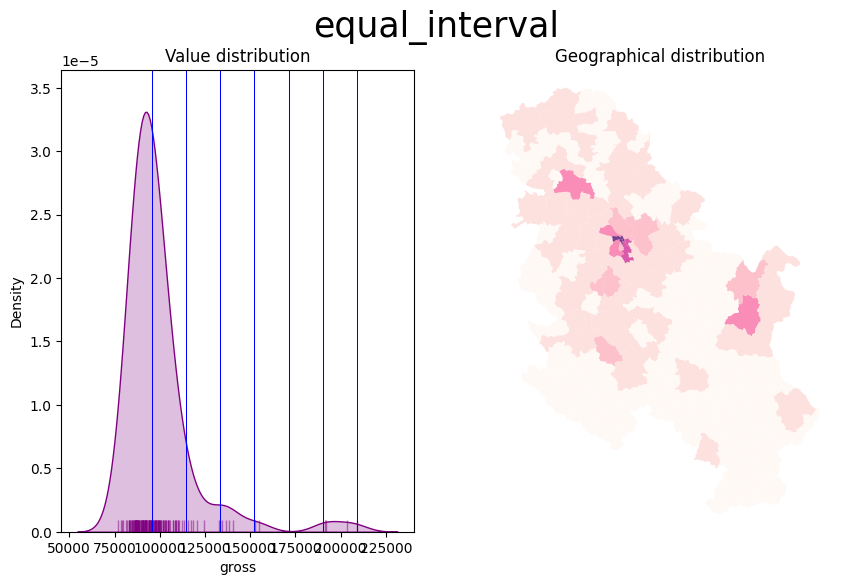
\includegraphics{labs/w02_maps_files/figure-pdf/cell-35-output-1.png}

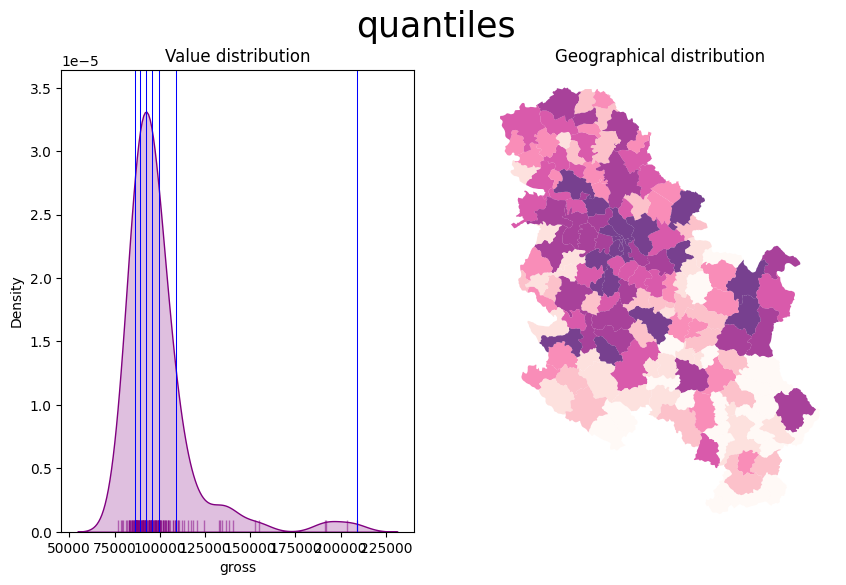
\includegraphics{labs/w02_maps_files/figure-pdf/cell-35-output-2.png}

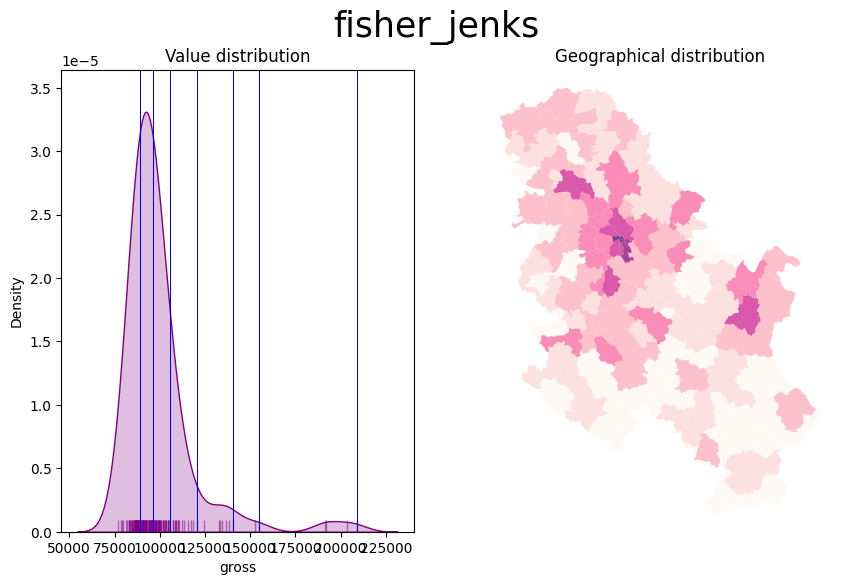
\includegraphics{labs/w02_maps_files/figure-pdf/cell-35-output-3.png}

Also consider the
\href{https://en.wikipedia.org/wiki/Modifiable_areal_unit_problem}{Modifiable
Areal Unit Problem} and how the geographies of the administrative
boundaries, in this case, may impact the visualisation.

For example, the most populated area is a municipality in the north that
corresponds to the city of Novi Sad. Let's have a look at the data

\begin{Shaded}
\begin{Highlighting}[]
\NormalTok{serbia\_admin[[}\StringTok{\textquotesingle{}name\textquotesingle{}}\NormalTok{, }\StringTok{\textquotesingle{}pop\textquotesingle{}}\NormalTok{, }\StringTok{\textquotesingle{}Province\textquotesingle{}}\NormalTok{]].sort\_values(by }\OperatorTok{=} \StringTok{\textquotesingle{}pop\textquotesingle{}}\NormalTok{, ascending }\OperatorTok{=} \VariableTok{False}\NormalTok{).iloc[:}\DecValTok{10}\NormalTok{]}
\end{Highlighting}
\end{Shaded}

\begin{longtable}[]{@{}llll@{}}
\toprule\noalign{}
& name & pop & Province \\
\midrule\noalign{}
\endhead
\bottomrule\noalign{}
\endlastfoot
48 & Novi Sad & 341625.0 & Južno-Bački \\
24 & Novi Beograd & 186667.0 & Grad Beograd \\
19 & Čukarica & 154854.0 & Grad Beograd \\
3 & Kragujevac & 154290.0 & Šumadijski \\
26 & Palilula & 148292.0 & Grad Beograd \\
34 & Zemun & 143173.0 & Grad Beograd \\
32 & Voždovac & 137315.0 & Grad Beograd \\
35 & Zvezdara & 130225.0 & Grad Beograd \\
39 & Leskovac & 123201.0 & Jablanički \\
120 & Subotica & 121250.0 & Severno-Bački \\
\end{longtable}

In our dataset, the city of Novi Sad is categorised as a municipality by
itself, because the administrative boundaries file is not updated. In
reality, ``since 2002, when the new statute of the city of Novi Sad came
into effect, Novi Sad is divided into two city municipalities,
Petrovaradin and Novi Sad. From 1989 until 2002, the name Municipality
of Novi Sad meant the whole territory of the present-day city of Novi
Sad.'' (see:
\href{https://en.wikipedia.org/wiki/City_municipality_of_Novi_Sad}{wikipedia}).

On the contrary, Grad Beograd, that is Belgrade, is correctly split into
different municipalities and its population, when visualised, is spread
out across the different geometries of its municipalities. In other
words, our map depends on the geometries of the areas and on how the
data was collected. While it could be that these areas were indeed
identified by population size in the first place, the point is that the
fact that Novi Sad is not split into more areas, as Belgrade is, makes
it stound out more clearly from the map (and to some extent a bit
unfairly)

This may happen with different types of data, particularly with
administrative boundaries and it is crucial to reflect on how Choropleth
maps may be impacted. One can look for more granular data or consider to
weight the continuous value with the extent of the area (i.e.~obtaining
density values).

\subsubsection{An alternative to scheme: ColorMap
Normalisation}\label{an-alternative-to-scheme-colormap-normalisation}

The \texttt{mpl.colors.Normalize} function in \texttt{matplotlib}
creates a normalization object, which adjusts data values into a range
that is ideal for colour mapping in a colormap. This function is
particularly beneficial in scenarios where precise control over the
mapping of data values to colour representations is needed.

When employed in a plotting function, this normalization object ensures
that the data values are scaled to fit a pre-defined range (for
instance, \texttt{norm\ =\ mpl.colors.Normalize(vmin=0,\ vmax=40)}). Any
values falling below 0 are mapped to the lowest colour on the colormap
scale, while values exceeding 40 are mapped to the highest colour. This
approach is especially useful when aiming to highlight differences
within a specific data range; it can significantly enhance the
visualization of data, by, for example, emphasizing temperature
variations between 0°C and 40°C. This becomes crucial in instances where
a few data points with high values (e.g., 50°C) might otherwise lead to
a less informative visualization if not `normalized' and treated as if
they corresponded to 40° C values.

For our dataset, we can use as \texttt{vmax} the value corresponding to
the 90th percentile.

\begin{Shaded}
\begin{Highlighting}[]
\NormalTok{serbia\_admin[}\StringTok{\textquotesingle{}pop\textquotesingle{}}\NormalTok{].quantile(}\FloatTok{0.90}\NormalTok{)}
\end{Highlighting}
\end{Shaded}

\begin{verbatim}
93014.0
\end{verbatim}

\begin{Shaded}
\begin{Highlighting}[]
\ImportTok{import}\NormalTok{ matplotlib }\ImportTok{as}\NormalTok{ mpl}
\NormalTok{fig, ax }\OperatorTok{=}\NormalTok{ plt.subplots(}\DecValTok{1}\NormalTok{, }\DecValTok{1}\NormalTok{)}
\NormalTok{vmin }\OperatorTok{=}\NormalTok{ serbia\_admin[}\StringTok{\textquotesingle{}pop\textquotesingle{}}\NormalTok{].}\BuiltInTok{min}\NormalTok{()}
\NormalTok{vmax }\OperatorTok{=}\NormalTok{ serbia\_admin[}\StringTok{\textquotesingle{}pop\textquotesingle{}}\NormalTok{].quantile(}\FloatTok{0.90}\NormalTok{) }\CommentTok{\# }
\NormalTok{norm }\OperatorTok{=}\NormalTok{ mpl.colors.Normalize(vmin}\OperatorTok{=}\NormalTok{vmin, vmax}\OperatorTok{=}\NormalTok{vmax)}
\NormalTok{serbia\_admin.plot(ax }\OperatorTok{=}\NormalTok{ ax, column}\OperatorTok{=}\StringTok{\textquotesingle{}pop\textquotesingle{}}\NormalTok{, cmap}\OperatorTok{=}\StringTok{\textquotesingle{}OrRd\textquotesingle{}}\NormalTok{, legend}\OperatorTok{=}\VariableTok{True}\NormalTok{, norm }\OperatorTok{=}\NormalTok{ norm)}
\end{Highlighting}
\end{Shaded}

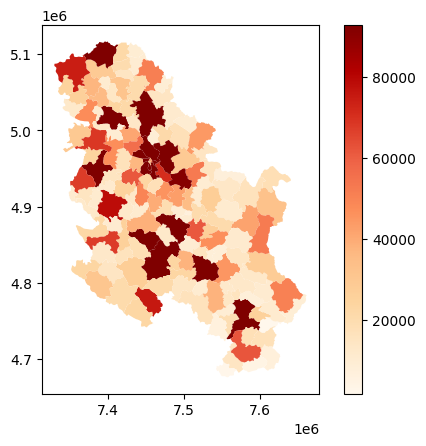
\includegraphics{labs/w02_maps_files/figure-pdf/cell-38-output-1.png}

\textbf{Important}:

When passing \texttt{norm} in the \texttt{plot} method, do not pass the
arguments to the \texttt{scheme} parameter. For continuous variables,
\texttt{norm} maps each value directly to a color, making discrete
categorization redundant. In other words, it allows for a direct mapping
of data values to the color map, eliminating the need for intermediary
classification schemes. \texttt{norm} ensures a smooth gradient in the
color map without artificially segmenting the data.

\subsubsection{Customising the colorbar}\label{customising-the-colorbar}

\begin{Shaded}
\begin{Highlighting}[]
\ImportTok{import}\NormalTok{ matplotlib.cm }\ImportTok{as}\NormalTok{ cm}

\NormalTok{fig, ax }\OperatorTok{=}\NormalTok{ plt.subplots(}\DecValTok{1}\NormalTok{, }\DecValTok{1}\NormalTok{)}
\NormalTok{cmap }\OperatorTok{=} \StringTok{\textquotesingle{}YlOrRd\textquotesingle{}}
\CommentTok{\# we leave the legend out}
\NormalTok{serbia\_admin.plot(column}\OperatorTok{=}\StringTok{\textquotesingle{}pop\textquotesingle{}}\NormalTok{, cmap}\OperatorTok{=}\NormalTok{cmap, norm }\OperatorTok{=}\NormalTok{ norm, ax}\OperatorTok{=}\NormalTok{ax)}

\CommentTok{\# we add the colorbar separately passing the norm and cmap}
\NormalTok{cbar }\OperatorTok{=}\NormalTok{ fig.colorbar(cm.ScalarMappable(norm}\OperatorTok{=}\NormalTok{norm, cmap}\OperatorTok{=}\NormalTok{cmap), ax }\OperatorTok{=}\NormalTok{ ax)}
\NormalTok{cbar.outline.set\_visible(}\VariableTok{False}\NormalTok{)}

\CommentTok{\# updating ticks VALUES}
\NormalTok{ticks }\OperatorTok{=}\NormalTok{ [norm.vmin, norm.vmax]}
\NormalTok{cbar.set\_ticks(ticks }\OperatorTok{=}\NormalTok{ ticks)}

\CommentTok{\# updating ticks LABELS}
\NormalTok{cbar.ax.set\_yticklabels([}\BuiltInTok{round}\NormalTok{(t,}\DecValTok{1}\NormalTok{) }\ControlFlowTok{for}\NormalTok{ t }\KeywordTok{in}\NormalTok{ ticks])}
\NormalTok{cbar.ax.set\_yticklabels([}\BuiltInTok{round}\NormalTok{(t,}\DecValTok{1}\NormalTok{) }\ControlFlowTok{if}\NormalTok{ t }\OperatorTok{\textless{}}\NormalTok{ norm.vmax }\ControlFlowTok{else} \StringTok{"\textgreater{}= "}\OperatorTok{+}\BuiltInTok{str}\NormalTok{(}\BuiltInTok{round}\NormalTok{(t,}\DecValTok{1}\NormalTok{)) }\ControlFlowTok{for}\NormalTok{ t }\KeywordTok{in}\NormalTok{ cbar.ax.get\_yticks()])}
\end{Highlighting}
\end{Shaded}

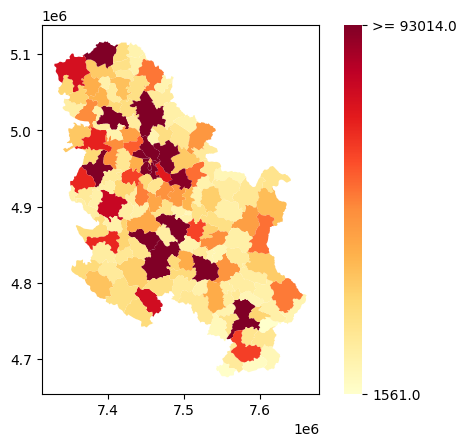
\includegraphics{labs/w02_maps_files/figure-pdf/cell-39-output-1.png}

Above, we removed the outline of the color bar. Then we set the tick
values to the min and the max population values, based on our norm
object. Then, for the vmax value's label we added a ``\textgreater='' to
remind us that other, higher values are displayed with the darkest
color.

\subsubsection{Varying alpha transparency based on an
array}\label{varying-alpha-transparency-based-on-an-array}

Finally, we can also convey variation in a continuous scale through
transparency. \texttt{alpha} doesn't expect column names, so we cannot
just pass the name of the column containing the variable. Instead, we
have to create an array from 0.0 to 1.0 values. To so we can a) use
normalisation methods, or b) rescale the original values within 0 to 1
based on the original min and max values.

For example, with square root normalization:

\begin{Shaded}
\begin{Highlighting}[]
\CommentTok{\# 1. Create an alpha array based on a normalized value (e.g., population)}
\ImportTok{import}\NormalTok{ numpy }\ImportTok{as}\NormalTok{ np}
\NormalTok{pop\_max }\OperatorTok{=}\NormalTok{ serbia\_admin[}\StringTok{\textquotesingle{}pop\textquotesingle{}}\NormalTok{].}\BuiltInTok{max}\NormalTok{()}
\NormalTok{alpha }\OperatorTok{=}\NormalTok{ np.sqrt(serbia\_admin[}\StringTok{\textquotesingle{}pop\textquotesingle{}}\NormalTok{] }\OperatorTok{/}\NormalTok{ pop\_max) }
\end{Highlighting}
\end{Shaded}

\begin{Shaded}
\begin{Highlighting}[]
\CommentTok{\# Plot with varying alpha values}
\NormalTok{fig, axes }\OperatorTok{=}\NormalTok{ plt.subplots(}\DecValTok{1}\NormalTok{, }\DecValTok{2}\NormalTok{, figsize}\OperatorTok{=}\NormalTok{(}\DecValTok{10}\NormalTok{, }\DecValTok{6}\NormalTok{))}
\NormalTok{serbia\_admin.plot(color }\OperatorTok{=} \StringTok{\textquotesingle{}blue\textquotesingle{}}\NormalTok{, ax}\OperatorTok{=}\NormalTok{axes[}\DecValTok{0}\NormalTok{], alpha}\OperatorTok{=}\NormalTok{alpha, edgecolor}\OperatorTok{=}\StringTok{\textquotesingle{}black\textquotesingle{}}\NormalTok{, linewidth }\OperatorTok{=} \FloatTok{0.3}\NormalTok{) }\CommentTok{\#one color}
\NormalTok{serbia\_admin.plot(cmap }\OperatorTok{=} \StringTok{\textquotesingle{}YlOrRd\textquotesingle{}}\NormalTok{, ax}\OperatorTok{=}\NormalTok{axes[}\DecValTok{1}\NormalTok{], alpha}\OperatorTok{=}\NormalTok{alpha, edgecolor}\OperatorTok{=}\StringTok{\textquotesingle{}red\textquotesingle{}}\NormalTok{, linewidth }\OperatorTok{=} \FloatTok{0.3}\NormalTok{) }\CommentTok{\#cmap}
\ControlFlowTok{for}\NormalTok{ ax }\KeywordTok{in}\NormalTok{ axes:}
\NormalTok{    ax.set\_axis\_off()}
\end{Highlighting}
\end{Shaded}

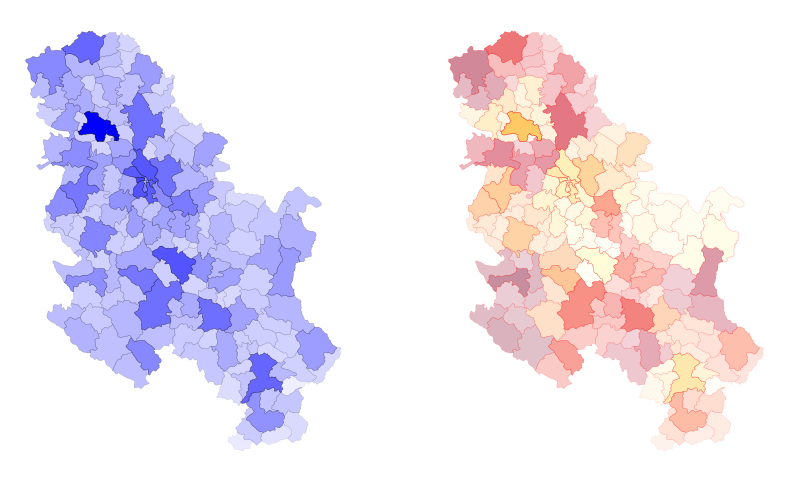
\includegraphics{labs/w02_maps_files/figure-pdf/cell-41-output-1.png}

\textbf{Important}:

\texttt{matplotlib} would not able to plot a color bar from variations
in the alpha value since no column is passed directly. We would need, in
this case, to build a color bar manually as demonstrated above.

\subsection{Choropleth Maps for Categorical
Variables}\label{choropleth-maps-for-categorical-variables}

A choropleth for categorical variables assigns a different color to
every potential value in the series based on certain colormaps
(\texttt{cmap}). We don't need to specify a scheme in this case, but
just to the categorical \texttt{column}. Using last's week GeoDataFrame,
we can plot terrorist attacks in Germany, for example, by group.

\begin{Shaded}
\begin{Highlighting}[]
\NormalTok{gdf }\OperatorTok{=}\NormalTok{ gpd.read\_file(}\StringTok{"../data/germany.shp"}\NormalTok{).to\_crs(germany\_crs)}
\NormalTok{fig, ax }\OperatorTok{=}\NormalTok{ plt.subplots(}\DecValTok{1}\NormalTok{, }\DecValTok{1}\NormalTok{, figsize}\OperatorTok{=}\NormalTok{(}\DecValTok{8}\NormalTok{, }\DecValTok{6}\NormalTok{))}
\NormalTok{gdf.plot(ax }\OperatorTok{=}\NormalTok{ ax, column }\OperatorTok{=} \StringTok{\textquotesingle{}gname\textquotesingle{}}\NormalTok{, legend }\OperatorTok{=} \VariableTok{True}\NormalTok{)}
\NormalTok{ax.set\_axis\_off()}
\NormalTok{title\_parameters }\OperatorTok{=}\NormalTok{ \{}\StringTok{\textquotesingle{}fontsize\textquotesingle{}}\NormalTok{:}\StringTok{\textquotesingle{}16\textquotesingle{}}\NormalTok{, }\StringTok{\textquotesingle{}fontname\textquotesingle{}}\NormalTok{:}\StringTok{\textquotesingle{}Times New Roman\textquotesingle{}}\NormalTok{\}}
\NormalTok{ax.set\_title(}\StringTok{"Terrorist Attacks in Germany, by Group"}\NormalTok{, }\OperatorTok{**}\NormalTok{title\_parameters) }\CommentTok{\#parameters as above}
\end{Highlighting}
\end{Shaded}

\begin{verbatim}
Text(0.5, 1.0, 'Terrorist Attacks in Germany, by Group')
\end{verbatim}

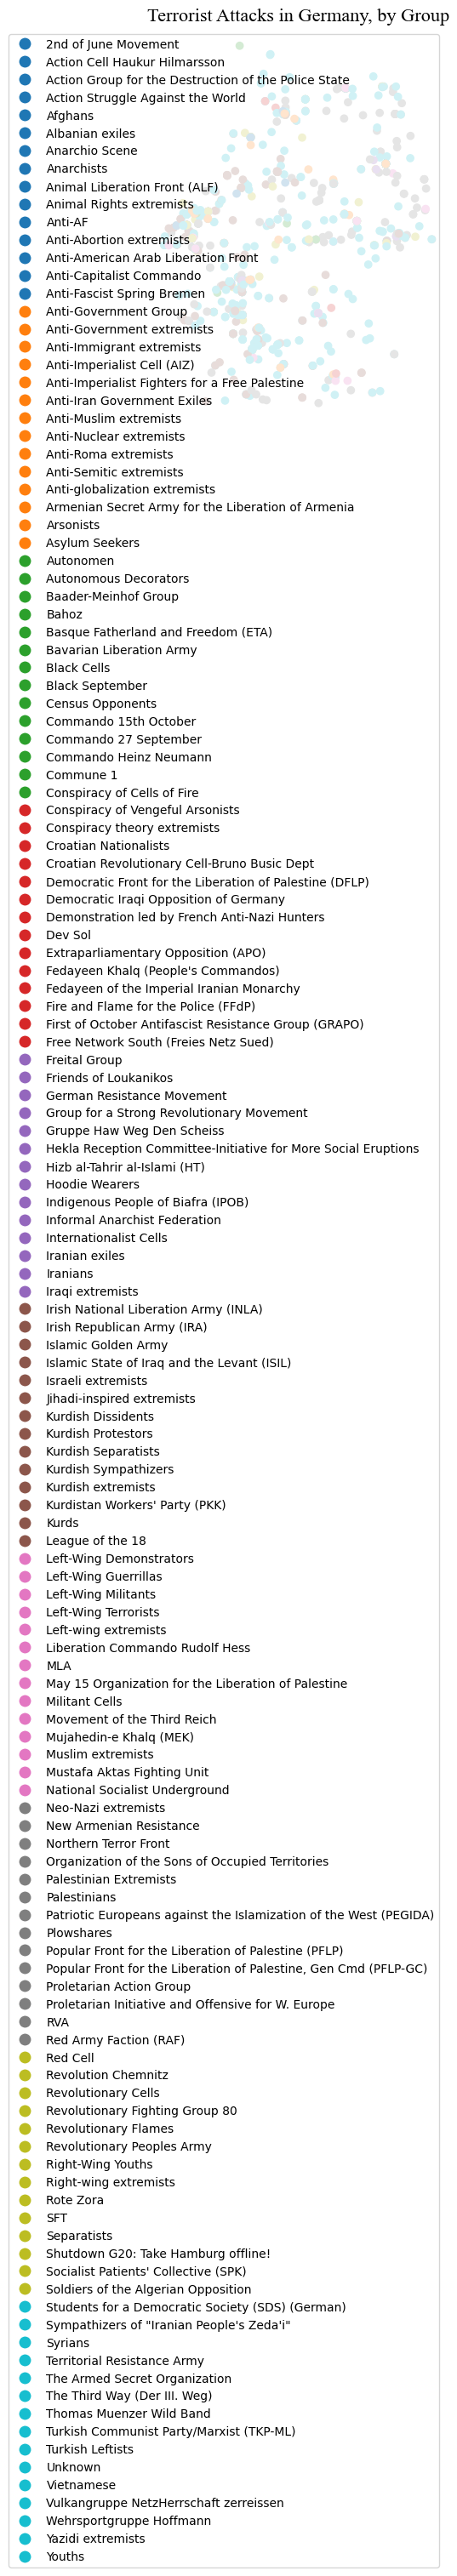
\includegraphics{labs/w02_maps_files/figure-pdf/cell-42-output-2.png}

The map above is what you would get from datasets that are not
cleaned/manipulated directly or when there are too many categories in
the selected column. First, let's get a slimmer slice of the gdf that
only contains attacks that cause a number of fatalities and wounded
higher than 10.

\begin{Shaded}
\begin{Highlighting}[]
\NormalTok{condition }\OperatorTok{=}\NormalTok{ (gdf.nkill }\OperatorTok{+}\NormalTok{ gdf.nwound) }\OperatorTok{\textgreater{}} \DecValTok{10}
\NormalTok{gdf\_filtered }\OperatorTok{=}\NormalTok{ gdf[condition].copy()}
\end{Highlighting}
\end{Shaded}

Then, let's build a function that creates a random color map based on
the number of categories. This creates random \texttt{HUE}-based colors:

\begin{Shaded}
\begin{Highlighting}[]
\CommentTok{\# Generate random colormap}
\KeywordTok{def}\NormalTok{ rand\_cmap(nlabels):}
    \CommentTok{""" }
\CommentTok{    It generates a categorical random color map, given the number of classes}
\CommentTok{    }
\CommentTok{    Parameters}
\CommentTok{    {-}{-}{-}{-}{-}{-}{-}{-}{-}{-}}
\CommentTok{    nlabels: int}
\CommentTok{        The number of categories to be coloured.}
\CommentTok{    type\_color: str \{"soft", "bright"\} }
\CommentTok{        It defines whether using bright or soft pastel colors, by limiting the RGB spectrum.}
\CommentTok{       }
\CommentTok{    Returns}
\CommentTok{    {-}{-}{-}{-}{-}{-}{-}}
\CommentTok{    cmap: matplotlib.colors.LinearSegmentedColormap}
\CommentTok{        The color map.}
\CommentTok{    """}   
    \CommentTok{\# Generate color map for bright colors, based on hsv}
\NormalTok{    randHSVcolors }\OperatorTok{=}\NormalTok{ [(np.random.uniform(low}\OperatorTok{=}\FloatTok{0.20}\NormalTok{, high}\OperatorTok{=}\FloatTok{0.80}\NormalTok{),}
\NormalTok{                          np.random.uniform(low}\OperatorTok{=}\FloatTok{0.20}\NormalTok{, high}\OperatorTok{=}\FloatTok{0.80}\NormalTok{),}
\NormalTok{                          np.random.uniform(low}\OperatorTok{=}\FloatTok{0.20}\NormalTok{, high}\OperatorTok{=} \FloatTok{0.80}\NormalTok{)) }\ControlFlowTok{for}\NormalTok{ i }\KeywordTok{in} \BuiltInTok{range}\NormalTok{(nlabels)]}

\NormalTok{    random\_colormap }\OperatorTok{=}\NormalTok{ LinearSegmentedColormap.from\_list(}\StringTok{\textquotesingle{}new\_map\textquotesingle{}}\NormalTok{, randHSVcolors, N}\OperatorTok{=}\NormalTok{nlabels)}
   
    \ControlFlowTok{return}\NormalTok{ random\_colormap }
\end{Highlighting}
\end{Shaded}

\begin{Shaded}
\begin{Highlighting}[]
\NormalTok{cmap }\OperatorTok{=}\NormalTok{ rand\_cmap(}\BuiltInTok{len}\NormalTok{(gdf\_filtered.gname.unique()))}
\NormalTok{cmap}
\end{Highlighting}
\end{Shaded}


\includegraphics{labs/w02_maps_files/figure-pdf/cell-45-output-1.png}

We also place the legend on the centre left. This is done automatically,
but the legend and its items can be manipulated directly. Legends in
\texttt{matplotlib} are extremely complex to personalise. However, do
have a look at
https://matplotlib.org/stable/api/\_as\_gen/matplotlib.pyplot.legend.html\#matplotlib.pyplot.legend
for both automatic and explicit manipulation.

\begin{Shaded}
\begin{Highlighting}[]
\NormalTok{legend\_kwds}\OperatorTok{=}\NormalTok{\{}\StringTok{"loc"}\NormalTok{: }\StringTok{"center left"}\NormalTok{, }\StringTok{"bbox\_to\_anchor"}\NormalTok{: (}\DecValTok{1}\NormalTok{, }\FloatTok{0.5}\NormalTok{)\}}
\end{Highlighting}
\end{Shaded}

\begin{Shaded}
\begin{Highlighting}[]
\NormalTok{fig, ax }\OperatorTok{=}\NormalTok{ plt.subplots(}\DecValTok{1}\NormalTok{, }\DecValTok{1}\NormalTok{, figsize}\OperatorTok{=}\NormalTok{(}\DecValTok{8}\NormalTok{, }\DecValTok{6}\NormalTok{))}
\NormalTok{gdf\_filtered.plot(ax }\OperatorTok{=}\NormalTok{ ax, column }\OperatorTok{=} \StringTok{\textquotesingle{}gname\textquotesingle{}}\NormalTok{, legend }\OperatorTok{=} \VariableTok{True}\NormalTok{, cmap }\OperatorTok{=}\NormalTok{ cmap, legend\_kwds }\OperatorTok{=}\NormalTok{ legend\_kwds)}
\NormalTok{title\_parameters }\OperatorTok{=}\NormalTok{ \{}\StringTok{\textquotesingle{}fontsize\textquotesingle{}}\NormalTok{:}\StringTok{\textquotesingle{}16\textquotesingle{}}\NormalTok{, }\StringTok{\textquotesingle{}fontname\textquotesingle{}}\NormalTok{:}\StringTok{\textquotesingle{}Times New Roman\textquotesingle{}}\NormalTok{\}}
\NormalTok{ax.set\_title(}\StringTok{"Terrorist Attacks in Germany, by Group"}\NormalTok{, }\OperatorTok{**}\NormalTok{title\_parameters) }\CommentTok{\#parameters as above}
\NormalTok{ctx.add\_basemap(ax, crs}\OperatorTok{=}\NormalTok{ gdf\_filtered.crs.to\_string(), source }\OperatorTok{=}\NormalTok{ ctx.providers.Esri.WorldGrayCanvas)}
\end{Highlighting}
\end{Shaded}

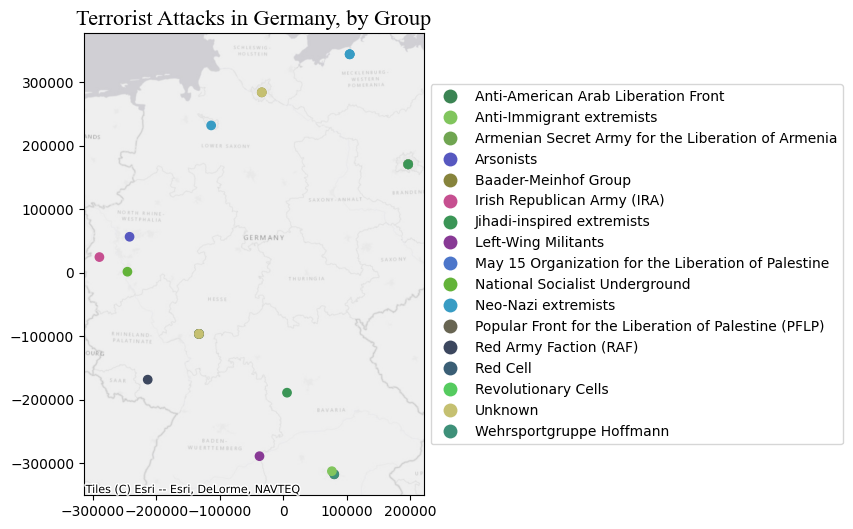
\includegraphics{labs/w02_maps_files/figure-pdf/cell-47-output-1.png}

We can also convey the impact of the events through the
\texttt{markersize}. This introduces the concept of \emph{cartogram}
(see below).

\begin{Shaded}
\begin{Highlighting}[]
\NormalTok{fig, ax }\OperatorTok{=}\NormalTok{ plt.subplots(}\DecValTok{1}\NormalTok{, }\DecValTok{1}\NormalTok{, figsize}\OperatorTok{=}\NormalTok{(}\DecValTok{8}\NormalTok{, }\DecValTok{6}\NormalTok{))}
\NormalTok{gdf\_filtered.plot(ax }\OperatorTok{=}\NormalTok{ ax, column }\OperatorTok{=} \StringTok{\textquotesingle{}gname\textquotesingle{}}\NormalTok{, markersize }\OperatorTok{=} \StringTok{\textquotesingle{}nwound\textquotesingle{}}\NormalTok{, legend }\OperatorTok{=} \VariableTok{True}\NormalTok{, cmap }\OperatorTok{=}\NormalTok{ cmap, legend\_kwds }\OperatorTok{=}\NormalTok{ legend\_kwds)}
\NormalTok{ax.set\_title(}\StringTok{"Terrorist Attacks in Germany, by Group"}\NormalTok{, }\OperatorTok{**}\NormalTok{title\_parameters) }\CommentTok{\#parameters as above}
\NormalTok{ctx.add\_basemap(ax, crs}\OperatorTok{=}\NormalTok{ gdf\_filtered.crs.to\_string(), source }\OperatorTok{=}\NormalTok{ ctx.providers.Esri.WorldGrayCanvas)}
\NormalTok{ax.set\_axis\_off()}
\end{Highlighting}
\end{Shaded}

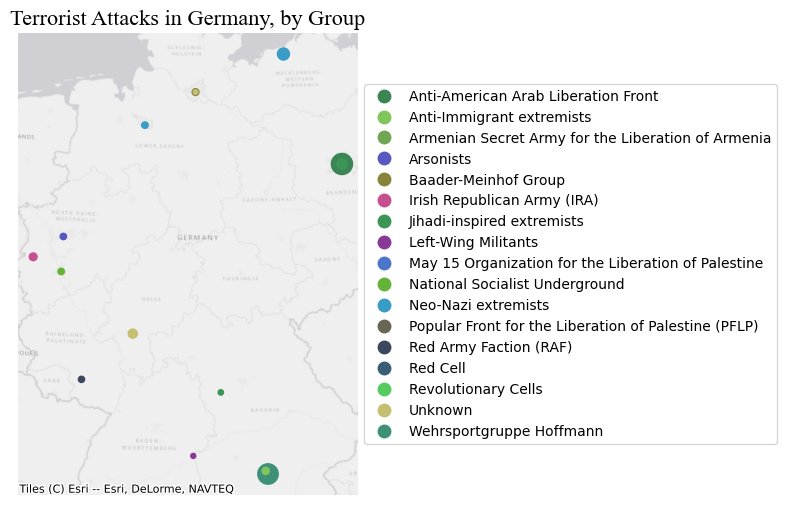
\includegraphics{labs/w02_maps_files/figure-pdf/cell-48-output-1.png}

\section{Part III: Cartograms - Manipulating the Geometry size for
showing the magnitude of a
value}\label{part-iii-cartograms---manipulating-the-geometry-size-for-showing-the-magnitude-of-a-value}

\href{https://www.data-to-viz.com/graph/cartogram.html}{Cartograms} are
maps that represent the spatial distribution of a variable not by
encoding it in a color palette but rather by modifying geographical
objects. There are many algorithms to distort the shapes of geographical
entities according to values, some of them are rather complex.

\subsection{Polygons}\label{polygons}

You can obtain cartograms for \texttt{Polygon} with \texttt{geoplot}:
see https://residentmario.github.io/geoplot/

\texttt{geoplot} functions pretty much work as \texttt{plot}

\begin{Shaded}
\begin{Highlighting}[]
\CommentTok{\# this library needs the GeoDataFrame to be reverted to WGS}
\NormalTok{ax }\OperatorTok{=}\NormalTok{ gplt.cartogram(serbia\_admin.to\_crs(wgs), scale}\OperatorTok{=}\StringTok{\textquotesingle{}pop\textquotesingle{}}\NormalTok{, projection}\OperatorTok{=}\NormalTok{gcrs.Mercator(), color }\OperatorTok{=} \StringTok{\textquotesingle{}darkblue\textquotesingle{}}\NormalTok{)}
\CommentTok{\# see for projections that work with gplt https://scitools.org.uk/cartopy/docs/v0.15/crs/projections.html}
\NormalTok{gplt.polyplot(serbia\_admin.to\_crs(wgs), facecolor}\OperatorTok{=}\StringTok{\textquotesingle{}lightgray\textquotesingle{}}\NormalTok{, edgecolor}\OperatorTok{=}\StringTok{\textquotesingle{}white\textquotesingle{}}\NormalTok{, ax}\OperatorTok{=}\NormalTok{ax, lw }\OperatorTok{=} \FloatTok{0.5}\NormalTok{) }\CommentTok{\# this is just for comparison}
\end{Highlighting}
\end{Shaded}

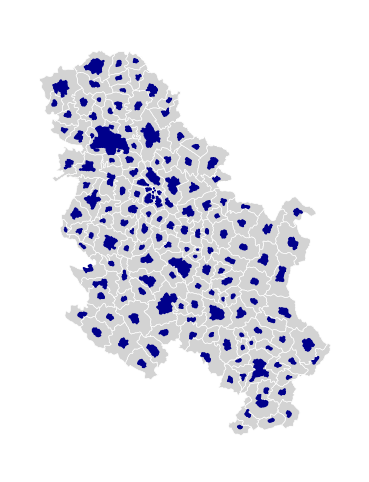
\includegraphics{labs/w02_maps_files/figure-pdf/cell-49-output-1.png}

\subsection{Points}\label{points}

For \texttt{Point} GeoDataFrames we can just go back to \texttt{plot}
and pass a column name to \texttt{markersize}.

\begin{Shaded}
\begin{Highlighting}[]
\NormalTok{attacks }\OperatorTok{=}\NormalTok{ pd.read\_csv(}\StringTok{"../data/GTD\_2022.csv"}\NormalTok{, low\_memory }\OperatorTok{=} \VariableTok{False}\NormalTok{)}
\NormalTok{country }\OperatorTok{=} \StringTok{\textquotesingle{}Germany\textquotesingle{}}

\NormalTok{df }\OperatorTok{=}\NormalTok{ attacks[attacks.country\_txt }\OperatorTok{==}\NormalTok{ country].copy()}
\NormalTok{wgs }\OperatorTok{=} \StringTok{\textquotesingle{}EPSG:4326\textquotesingle{}}
\NormalTok{germany\_crs }\OperatorTok{=} \StringTok{\textquotesingle{}EPSG:4839\textquotesingle{}}
\NormalTok{gdf }\OperatorTok{=}\NormalTok{ gpd.GeoDataFrame(df, geometry}\OperatorTok{=}\NormalTok{gpd.points\_from\_xy(df.longitude, df.latitude), crs }\OperatorTok{=}\NormalTok{ wgs)}
\NormalTok{gdf }\OperatorTok{=}\NormalTok{ gdf.to\_crs(germany\_crs)}
\end{Highlighting}
\end{Shaded}

\begin{Shaded}
\begin{Highlighting}[]
\NormalTok{fig, ax }\OperatorTok{=}\NormalTok{ plt.subplots(}\DecValTok{1}\NormalTok{, }\DecValTok{1}\NormalTok{, figsize}\OperatorTok{=}\NormalTok{(}\DecValTok{8}\NormalTok{, }\DecValTok{6}\NormalTok{))}
\NormalTok{gdf.plot(ax }\OperatorTok{=}\NormalTok{ ax, markersize }\OperatorTok{=} \StringTok{\textquotesingle{}nwound\textquotesingle{}}\NormalTok{, color }\OperatorTok{=} \StringTok{\textquotesingle{}purple\textquotesingle{}}\NormalTok{, legend }\OperatorTok{=} \VariableTok{True}\NormalTok{)}
\NormalTok{ax.set\_axis\_off()}
\end{Highlighting}
\end{Shaded}


\includegraphics{labs/w02_maps_files/figure-pdf/cell-51-output-1.png}

One can also convert polygons into points by using their centroids, and
then define the size of the dot proportionally to the value of the
variable we want to display.

\subsection{LineString}\label{linestring}

For \texttt{LineString} we pass the column name to \texttt{linewidth}.

Let's load a shapefile of lines. These lines represent frequency of
train connections from/to train stations in the region of Liguria
(Italy) to other stations within or outside the region. Each line refers
to a connection between two specific stations, through a certain type of
service and contains information about the frequency of that type of
service. For example, the cities of Savona and Finale Ligure might be
connected by 5 InterCity trains and 50 regional services. These services
correspond to 2 different records.

\begin{Shaded}
\begin{Highlighting}[]
\NormalTok{trains\_freq }\OperatorTok{=}\NormalTok{ gpd.read\_file(}\StringTok{"../data/trains\_liguria.shp"}\NormalTok{ )}
\NormalTok{trains\_freq.crs}
\end{Highlighting}
\end{Shaded}

\begin{verbatim}
<Projected CRS: EPSG:3003>
Name: Monte Mario / Italy zone 1
Axis Info [cartesian]:
- X[east]: Easting (metre)
- Y[north]: Northing (metre)
Area of Use:
- name: Italy - onshore and offshore - west of 12°E.
- bounds: (5.93, 36.53, 12.0, 47.04)
Coordinate Operation:
- name: Italy zone 1
- method: Transverse Mercator
Datum: Monte Mario
- Ellipsoid: International 1924
- Prime Meridian: Greenwich
\end{verbatim}

Let's check the type of services contained here.

\begin{Shaded}
\begin{Highlighting}[]
\NormalTok{trains\_freq[}\StringTok{\textquotesingle{}train\_type\textquotesingle{}}\NormalTok{].unique()}
\end{Highlighting}
\end{Shaded}

\begin{verbatim}
array(['REG', 'IC', 'FB', 'ICN', 'U', 'EC/EN', 'AV'], dtype=object)
\end{verbatim}

We have: - `REG': regional trains. - `IC': intercity trains. - `FB':
similar to IC, but slightly faster. - `ICN': sleeper trains. - `U':
urban trains (Genoa). - `EC/EN': international trains. - `AV':
High-speed trains.

Let's keep just regional, intercity, and high-speed trains.

\begin{Shaded}
\begin{Highlighting}[]
\NormalTok{to\_keep }\OperatorTok{=}\NormalTok{ [}\StringTok{\textquotesingle{}REG\textquotesingle{}}\NormalTok{, }\StringTok{\textquotesingle{}IC\textquotesingle{}}\NormalTok{, }\StringTok{\textquotesingle{}AV\textquotesingle{}}\NormalTok{]}
\NormalTok{trains\_freq }\OperatorTok{=}\NormalTok{ trains\_freq[trains\_freq[}\StringTok{\textquotesingle{}train\_type\textquotesingle{}}\NormalTok{].isin(to\_keep)]}
\end{Highlighting}
\end{Shaded}

The usage of \texttt{linewdith} is a bit different from
\texttt{markersize} for some reason. We have to pass an \texttt{array}
of N values, where N is equal to the GeoDataFrame size. In other words,
we have to pass the column we want to use to regulate the line width
directly as a list/array. Specifying the column name is not enough.

\begin{Shaded}
\begin{Highlighting}[]
\NormalTok{fig, ax }\OperatorTok{=}\NormalTok{ plt.subplots(}\DecValTok{1}\NormalTok{, }\DecValTok{1}\NormalTok{, figsize}\OperatorTok{=}\NormalTok{(}\DecValTok{10}\NormalTok{, }\DecValTok{15}\NormalTok{))}
\NormalTok{trains\_freq.plot(ax }\OperatorTok{=}\NormalTok{ ax, linewidth }\OperatorTok{=}\NormalTok{ trains\_freq[}\StringTok{\textquotesingle{}freq\textquotesingle{}}\NormalTok{])}
\NormalTok{ax.set\_axis\_off()}
\end{Highlighting}
\end{Shaded}

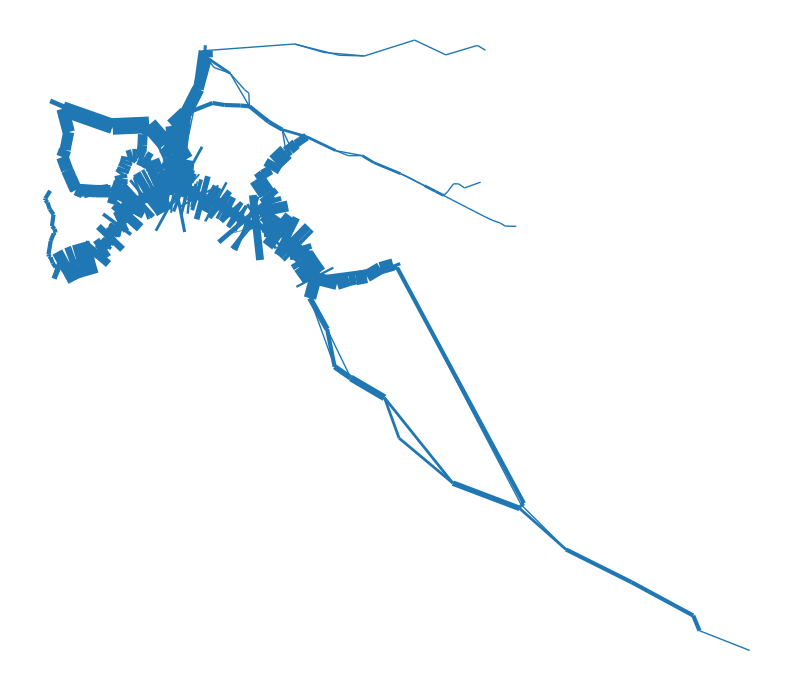
\includegraphics{labs/w02_maps_files/figure-pdf/cell-55-output-1.png}

As you can see, the default arguments and simply passing the column
values do not produce pretty results. The first thing to look at is the
values that are passed to \texttt{linewidth}. In some cases, the min and
max values, as well as their distribution, are not ideal for visually
conveying the magnitude of the variable attached to the geometry. One
option is to use a multiplier factor (see below), or to rescale the
values from 0 to 1, for example, and then, again, if necessary use a
multiplier.

\begin{Shaded}
\begin{Highlighting}[]
\NormalTok{fig, ax }\OperatorTok{=}\NormalTok{ plt.subplots(}\DecValTok{1}\NormalTok{, }\DecValTok{1}\NormalTok{, figsize}\OperatorTok{=}\NormalTok{(}\DecValTok{15}\NormalTok{, }\DecValTok{20}\NormalTok{))}
\NormalTok{lw }\OperatorTok{=}\NormalTok{ trains\_freq[}\StringTok{\textquotesingle{}freq\textquotesingle{}}\NormalTok{] }\OperatorTok{*} \FloatTok{0.15}
\NormalTok{trains\_freq.plot(ax }\OperatorTok{=}\NormalTok{ ax, linewidth }\OperatorTok{=}\NormalTok{ lw, capstyle }\OperatorTok{=} \StringTok{\textquotesingle{}round\textquotesingle{}}\NormalTok{, joinstyle }\OperatorTok{=} \StringTok{\textquotesingle{}round\textquotesingle{}}\NormalTok{, column }\OperatorTok{=} \StringTok{\textquotesingle{}train\_type\textquotesingle{}}\NormalTok{, legend }\OperatorTok{=} \VariableTok{True}\NormalTok{)}
\NormalTok{ctx.add\_basemap(ax, crs}\OperatorTok{=}\NormalTok{ trains\_freq.crs.to\_string(), source }\OperatorTok{=}\NormalTok{ ctx.providers.Esri.WorldGrayCanvas)}
\NormalTok{ax.set\_axis\_off()}
\end{Highlighting}
\end{Shaded}

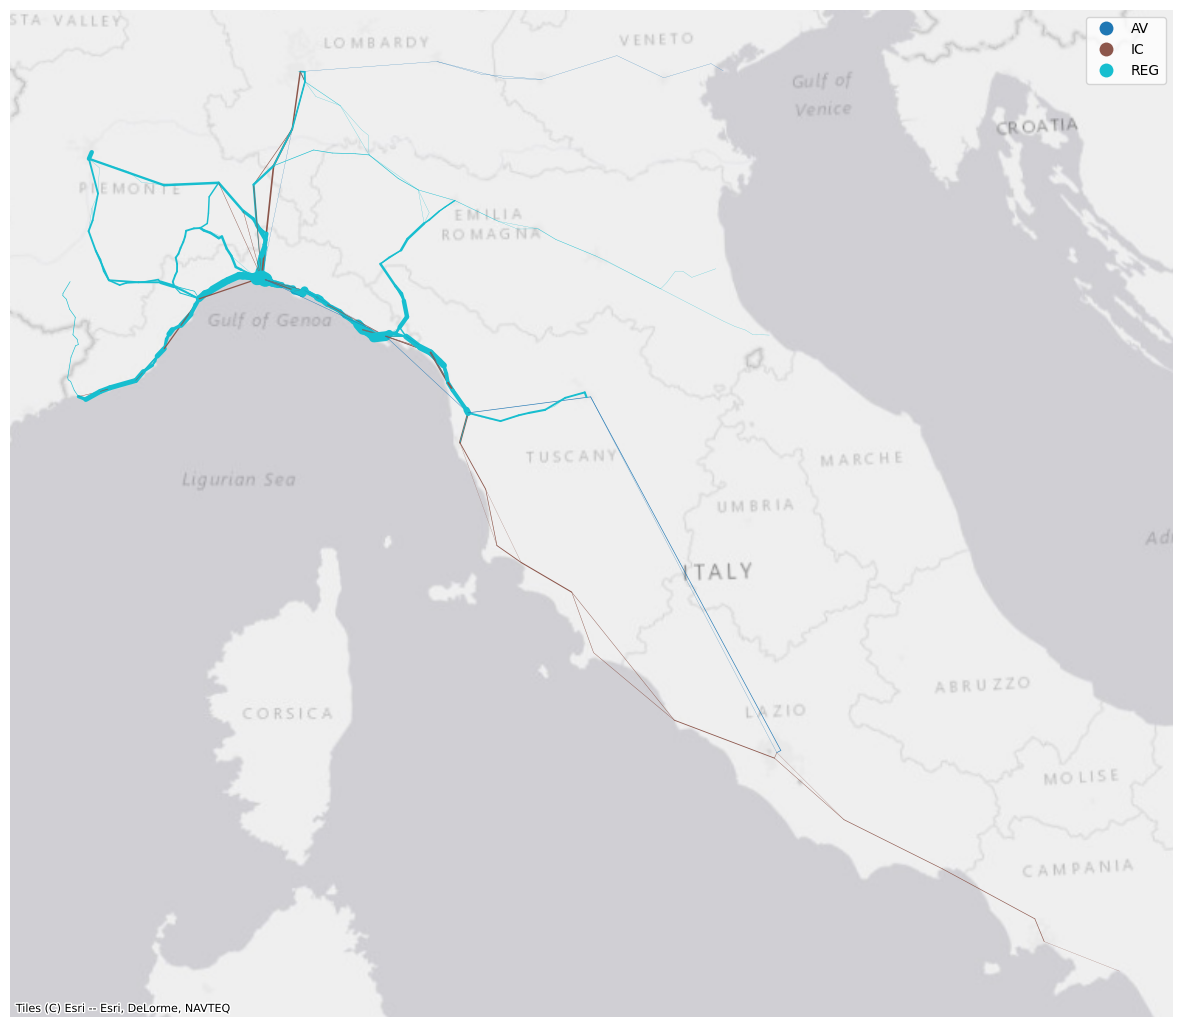
\includegraphics{labs/w02_maps_files/figure-pdf/cell-56-output-1.png}

While this looks a bit better, this visualisation is not ideal because
the frequencies are not snapped to the actual railway network. The lines
represent, instead, connection between train stops and therefore their
coordinates only include the ones corresponding to the stations where
the different services call at. One can devise approaches to:

\begin{itemize}
\tightlist
\item
  Assigning the frequencies, or any other value, to the corresponding
  infrastructure's section. For example, the railway section between two
  stations could be associated with a value representing the total
  number of regional/local services travelling along it.
\item
  Smoothing the lines representing the services by adding further
  coordinates along the line.
\end{itemize}

Both these processes go beyond the scopes of this lab and require
several considerations depending on the data, the scale, and what
information one wants to displays.

\textbf{Exercise}:

Today we've seen how to exploit \texttt{matplotlib} to plot
\texttt{GeoDataFrame} layers. Go through the notebook again if you feel
that there's something you need to review. You are not expected to
remember each step/method/parameter. Rather, this notebook should be
used as a reference for producing maps in Python. Do keep in mind that
most of the maps above have been produced with just a bunch of rows, so
each of them can be improved and embellished with some more effort.

Now, if you are not overwhelmed, have a look at the very last map and
produce some nice visualisation using the same data. You can further
improve its clarity, add a legend that refers to the line width,
visualise only a certain type of services, or add information/context,
for example. In the folder \texttt{\textbackslash{}data} you can also
find a \texttt{.shp} file containing all the train stations in Italy,
should you need that.

\subsubsection{\texorpdfstring{Saving figures (check
\href{https://matplotlib.org/stable/api/_as_gen/matplotlib.pyplot.savefig.html}{here
for
details})}{Saving figures (check here for details)}}\label{saving-figures-check-here-for-details}

\begin{Shaded}
\begin{Highlighting}[]
\NormalTok{fig.savefig(}\StringTok{"fig1.pdf"}\NormalTok{, dpi}\OperatorTok{=}\StringTok{\textquotesingle{}figure\textquotesingle{}}\NormalTok{, }\BuiltInTok{format}\OperatorTok{=}\StringTok{"pdf"}\NormalTok{, bbox\_inches }\OperatorTok{=} \StringTok{\textquotesingle{}tight\textquotesingle{}}\NormalTok{)}
\end{Highlighting}
\end{Shaded}

\bookmarksetup{startatroot}

\chapter{Panel spatial lags}\label{panel-spatial-lags}

This document shows how one can calculate spatial lag of a series of
variables over several periods of time, assuming the geography (e.g.,
\(W\)) remains constant.

\begin{Shaded}
\begin{Highlighting}[]
\ImportTok{import}\NormalTok{ pandas}
\ImportTok{import}\NormalTok{ geopandas}
\ImportTok{from}\NormalTok{ libpysal }\ImportTok{import}\NormalTok{ graph}
\end{Highlighting}
\end{Shaded}

\textbf{NOTE} - This implementation relies on the new \texttt{graph}
structures for spatial weights in PySAL. For that reason, a recent
version of the library is required.

\section{Data}\label{data}

\begin{itemize}
\tightlist
\item
  Tabular data
\end{itemize}

Note we drop the names as they're irrelevant here (we have unique IDs)
and index the table on region ID and year. The resulting table contains
only the variables to lag as columns.

\begin{Shaded}
\begin{Highlighting}[]
\NormalTok{panel }\OperatorTok{=}\NormalTok{ (}
\NormalTok{    pandas.read\_csv(}
        \StringTok{\textquotesingle{}spatial\_lag\_panel\_data.csv\textquotesingle{}}\NormalTok{, }
\NormalTok{        encoding }\OperatorTok{=} \StringTok{\textquotesingle{}ISO{-}8859{-}9\textquotesingle{}} \CommentTok{\# Turkish encoding}
\NormalTok{    )}
\NormalTok{    .set\_index([}\StringTok{\textquotesingle{}asdf\_id\textquotesingle{}}\NormalTok{, }\StringTok{\textquotesingle{}year\textquotesingle{}}\NormalTok{])}
\NormalTok{    .drop(columns}\OperatorTok{=}\NormalTok{[}\StringTok{\textquotesingle{}shapeName\textquotesingle{}}\NormalTok{])}
\NormalTok{)}
\end{Highlighting}
\end{Shaded}

\begin{itemize}
\tightlist
\item
  Geographic data
\end{itemize}

\begin{Shaded}
\begin{Highlighting}[]
\NormalTok{geo }\OperatorTok{=}\NormalTok{ geopandas.read\_file(}\StringTok{\textquotesingle{}TUR\_ADM1.geojson\textquotesingle{}}\NormalTok{).set\_index(}\StringTok{\textquotesingle{}asdf\_id\textquotesingle{}}\NormalTok{)}
\end{Highlighting}
\end{Shaded}

\begin{verbatim}
ERROR 1: PROJ: proj_create_from_database: Open of /opt/conda/envs/gds/share/proj failed
\end{verbatim}

\section{Lag computation}\label{lag-computation}

First, we compute the spatial weights we will use. In this example, we
pick queen contiguity, although other criteria are available and
possibly valid too.

\begin{Shaded}
\begin{Highlighting}[]
\NormalTok{w }\OperatorTok{=}\NormalTok{ (}
\NormalTok{    graph.Graph.build\_contiguity(geo, rook}\OperatorTok{=}\VariableTok{False}\NormalTok{)}
\NormalTok{    .transform(}\StringTok{\textquotesingle{}R\textquotesingle{}}\NormalTok{)}
\NormalTok{)}
\end{Highlighting}
\end{Shaded}

Now we're ready to compute the lags. We approach this as a nested
\texttt{for} loop, where we iterate through every year and, within that,
through every variable. To make computation more efficient, we first
generate the frame where results will be stored (\texttt{lags}).

\begin{Shaded}
\begin{Highlighting}[]
\NormalTok{lags }\OperatorTok{=}\NormalTok{ pandas.DataFrame(index}\OperatorTok{=}\NormalTok{panel.index, columns}\OperatorTok{=}\NormalTok{panel.columns)}

\ControlFlowTok{for}\NormalTok{ year }\KeywordTok{in}\NormalTok{ panel.index.get\_level\_values(}\StringTok{\textquotesingle{}year\textquotesingle{}}\NormalTok{).unique():}
    \ControlFlowTok{for}\NormalTok{ var }\KeywordTok{in}\NormalTok{ lags.columns:}
\NormalTok{        vals }\OperatorTok{=}\NormalTok{ panel.loc[pandas.IndexSlice[:, year], var]}
\NormalTok{        lags.loc[vals.index, var] }\OperatorTok{=}\NormalTok{ w.lag(vals)}
\end{Highlighting}
\end{Shaded}

We can now write the lagged values to disk:

\begin{Shaded}
\begin{Highlighting}[]
\NormalTok{lags.to\_csv(}\StringTok{\textquotesingle{}lagged.csv\textquotesingle{}}\NormalTok{)}
\end{Highlighting}
\end{Shaded}

\bookmarksetup{startatroot}

\chapter{}\label{section}

\begin{Shaded}
\begin{Highlighting}[]
\ImportTok{import}\NormalTok{ numpy }\ImportTok{as}\NormalTok{ np}
\ImportTok{import}\NormalTok{ pandas }\ImportTok{as}\NormalTok{ pd}
\ImportTok{import}\NormalTok{ seaborn }\ImportTok{as}\NormalTok{ sns}
\NormalTok{sns.set\_style(}\StringTok{"darkgrid"}\NormalTok{)}
\NormalTok{sns.set\_context(context}\OperatorTok{=}\StringTok{"paper"}\NormalTok{, font\_scale}\OperatorTok{=}\FloatTok{1.5}\NormalTok{, rc}\OperatorTok{=}\VariableTok{None}\NormalTok{)}
\NormalTok{sns.}\BuiltInTok{set}\NormalTok{(font}\OperatorTok{=}\StringTok{"serif"}\NormalTok{)}
\ImportTok{import}\NormalTok{ seaborn}

\ImportTok{import}\NormalTok{ geopandas }\ImportTok{as}\NormalTok{ gpd}
\ImportTok{import}\NormalTok{ matplotlib.pyplot }\ImportTok{as}\NormalTok{ plt}

\ImportTok{import}\NormalTok{ libpysal}
\ImportTok{from}\NormalTok{ libpysal  }\ImportTok{import}\NormalTok{ weights}
\ImportTok{from}\NormalTok{ pysal.explore }\ImportTok{import}\NormalTok{ esda }
\ImportTok{import}\NormalTok{ esda}
\ImportTok{from}\NormalTok{ esda.moran }\ImportTok{import}\NormalTok{ Moran, Moran\_Local}

\ImportTok{import}\NormalTok{ splot}
\ImportTok{from}\NormalTok{ splot.esda }\ImportTok{import}\NormalTok{ moran\_scatterplot, plot\_moran, lisa\_cluster}
\ImportTok{from}\NormalTok{ splot.libpysal }\ImportTok{import}\NormalTok{ plot\_spatial\_weights}

\ImportTok{from}\NormalTok{ giddy.directional }\ImportTok{import}\NormalTok{ Rose}
\ImportTok{import}\NormalTok{ os}

\ImportTok{from}\NormalTok{ numpy.random }\ImportTok{import}\NormalTok{ seed}
\NormalTok{seed(}\DecValTok{12345}\NormalTok{)}
\end{Highlighting}
\end{Shaded}

\begin{verbatim}
C:\Users\uursavas\AppData\Local\anaconda3\Lib\site-packages\spaghetti\network.py:40: FutureWarning: The next major release of pysal/spaghetti (2.0.0) will drop support for all ``libpysal.cg`` geometries. This change is a first step in refactoring ``spaghetti`` that is expected to result in dramatically reduced runtimes for network instantiation and operations. Users currently requiring network and point pattern input as ``libpysal.cg`` geometries should prepare for this simply by converting to ``shapely`` geometries.
  warnings.warn(dep_msg, FutureWarning, stacklevel=1)
\end{verbatim}

\begin{Shaded}
\begin{Highlighting}[]
\NormalTok{os.chdir(}\StringTok{\textquotesingle{}F:/projects/2024/ntl\_2\textquotesingle{}}\NormalTok{)}
\end{Highlighting}
\end{Shaded}

\begin{Shaded}
\begin{Highlighting}[]
\NormalTok{gini }\OperatorTok{=}\NormalTok{ pd.read\_csv(}\StringTok{"F:/projects/2024/ntl\_2/gini\_map.csv"}\NormalTok{, encoding}\OperatorTok{=}\StringTok{\textquotesingle{}unicode\_escape\textquotesingle{}}\NormalTok{)}
\end{Highlighting}
\end{Shaded}

\begin{Shaded}
\begin{Highlighting}[]
\NormalTok{geojson\_data }\OperatorTok{=}\NormalTok{ gpd.read\_file(}\StringTok{"F:/projects/2024/informal/TUR\_ADM1.geojson"}\NormalTok{)}
\end{Highlighting}
\end{Shaded}

\begin{Shaded}
\begin{Highlighting}[]
\NormalTok{merged\_data }\OperatorTok{=}\NormalTok{ pd.merge(geojson\_data, gini, how}\OperatorTok{=}\StringTok{\textquotesingle{}left\textquotesingle{}}\NormalTok{, left\_on}\OperatorTok{=}\StringTok{\textquotesingle{}asdf\_id\textquotesingle{}}\NormalTok{, right\_on}\OperatorTok{=}\StringTok{\textquotesingle{}asdf\_id\textquotesingle{}}\NormalTok{)}
\end{Highlighting}
\end{Shaded}

\begin{Shaded}
\begin{Highlighting}[]
\NormalTok{fig, ax }\OperatorTok{=}\NormalTok{ plt.subplots(figsize}\OperatorTok{=}\NormalTok{(}\DecValTok{12}\NormalTok{,}\DecValTok{8}\NormalTok{))}
\NormalTok{merged\_data.plot(column}\OperatorTok{=}\StringTok{"GINI\_area"}\NormalTok{, scheme}\OperatorTok{=}\StringTok{\textquotesingle{}NaturalBreaks\textquotesingle{}}\NormalTok{, k}\OperatorTok{=}\DecValTok{5}\NormalTok{, cmap}\OperatorTok{=}\StringTok{\textquotesingle{}coolwarm\textquotesingle{}}\NormalTok{, legend}\OperatorTok{=}\VariableTok{True}\NormalTok{, ax}\OperatorTok{=}\NormalTok{ax)}
\NormalTok{plt.title(}\StringTok{\textquotesingle{}Spatial distribution of GINI in 2019\textquotesingle{}}\NormalTok{)}
\NormalTok{plt.tight\_layout()}
\NormalTok{ax.axis(}\StringTok{"off"}\NormalTok{)}
\NormalTok{plt.savefig(}\StringTok{\textquotesingle{}gini\_distribution\_2019.png\textquotesingle{}}\NormalTok{, }\BuiltInTok{format}\OperatorTok{=}\StringTok{\textquotesingle{}png\textquotesingle{}}\NormalTok{, dpi}\OperatorTok{=}\DecValTok{300}\NormalTok{)  }\CommentTok{\# Saves the figure to a PNG file with high resolution}


\NormalTok{plt.show()}
\end{Highlighting}
\end{Shaded}

\begin{verbatim}
C:\Users\uursavas\AppData\Local\anaconda3\Lib\site-packages\sklearn\cluster\_kmeans.py:1436: UserWarning: KMeans is known to have a memory leak on Windows with MKL, when there are less chunks than available threads. You can avoid it by setting the environment variable OMP_NUM_THREADS=1.
  warnings.warn(
\end{verbatim}

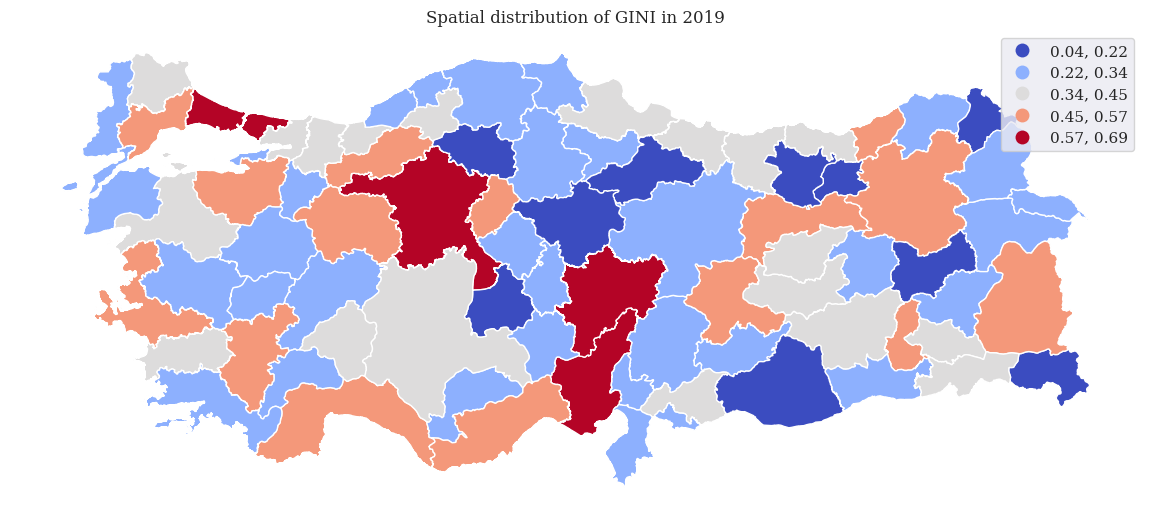
\includegraphics{labs/gini_map_2019_files/figure-pdf/cell-7-output-2.png}

\bookmarksetup{startatroot}

\chapter{}\label{section-1}

\begin{Shaded}
\begin{Highlighting}[]
\ImportTok{import}\NormalTok{ pandas}
\ImportTok{import}\NormalTok{ geopandas}
\ImportTok{from}\NormalTok{ libpysal }\ImportTok{import}\NormalTok{ graph}
\ImportTok{import}\NormalTok{ os}
\ImportTok{import}\NormalTok{ geopandas }\ImportTok{as}\NormalTok{ gpd}
\end{Highlighting}
\end{Shaded}

\begin{Shaded}
\begin{Highlighting}[]
\NormalTok{os.chdir(}\StringTok{\textquotesingle{}F:/projects/2024/ursavas\_alahmadi\_chen/data/ntl\_data\textquotesingle{}}\NormalTok{)}
\end{Highlighting}
\end{Shaded}

\begin{Shaded}
\begin{Highlighting}[]
\NormalTok{panel }\OperatorTok{=}\NormalTok{ (}
\NormalTok{    pandas.read\_csv(}
        \StringTok{\textquotesingle{}spatial.csv\textquotesingle{}}\NormalTok{, }
\NormalTok{        encoding }\OperatorTok{=} \StringTok{\textquotesingle{}ISO{-}8859{-}9\textquotesingle{}} \CommentTok{\# Turkish encoding}
\NormalTok{    )}
\NormalTok{    .set\_index([}\StringTok{\textquotesingle{}asdf\_id\textquotesingle{}}\NormalTok{, }\StringTok{\textquotesingle{}year\textquotesingle{}}\NormalTok{])}
    
\NormalTok{)}
\end{Highlighting}
\end{Shaded}

\begin{Shaded}
\begin{Highlighting}[]
\NormalTok{geo }\OperatorTok{=}\NormalTok{ gpd.read\_file(}\StringTok{"F:/projects/2024/informal/TUR\_ADM1.geojson"}\NormalTok{)}
\end{Highlighting}
\end{Shaded}

\begin{Shaded}
\begin{Highlighting}[]
\NormalTok{w }\OperatorTok{=}\NormalTok{ (}
\NormalTok{    graph.Graph.build\_contiguity(geo, rook}\OperatorTok{=}\VariableTok{False}\NormalTok{)}
\NormalTok{    .transform(}\StringTok{\textquotesingle{}R\textquotesingle{}}\NormalTok{)}
\NormalTok{)}
\end{Highlighting}
\end{Shaded}

\begin{Shaded}
\begin{Highlighting}[]
\NormalTok{w.neighbors}
\end{Highlighting}
\end{Shaded}

\begin{verbatim}
{0: (36, 41, 46, 57, 61, 63),
 1: (25, 32, 41, 54, 80),
 2: (19, 24, 31, 38, 52, 53, 74),
 3: (17, 30, 37, 44, 59, 75),
 4: (23, 66, 71, 77),
 5: (19, 38, 43, 52, 57, 58),
 6: (11, 30, 64),
 7: (24, 40, 55, 58),
 8: (20, 21, 40, 53, 55),
 9: (10, 18, 22, 31, 48, 50, 52),
 10: (9, 50, 52, 60, 61),
 11: (6, 30, 44),
 12: (42, 45, 78),
 13: (17, 25, 56, 59, 67, 79),
 14: (29, 30, 34, 64, 72),
 15: (18, 20, 31, 51, 53, 65),
 16: (25, 28, 29, 30, 59, 73),
 17: (3, 13, 59, 67, 75),
 18: (9, 15, 22, 26, 31, 42, 65, 78),
 19: (2, 5, 24, 38, 58),
 20: (8, 15, 51, 53, 76),
 21: (8, 27, 70),
 22: (9, 18, 23, 42, 45, 48),
 23: (4, 22, 45, 48, 66, 68, 77),
 24: (2, 7, 19, 55, 58, 74),
 25: (1, 13, 16, 28, 54, 56, 59, 80),
 26: (18, 65, 78),
 27: (21, 49, 70),
 28: (16, 25, 29, 54, 73),
 29: (14, 16, 28, 30, 33, 34, 54, 69, 73),
 30: (3, 6, 11, 14, 16, 29, 44, 59, 64),
 31: (2, 9, 15, 18, 52, 53),
 32: (1, 36, 41, 47, 63, 80),
 33: (29, 34, 62, 69, 72),
 34: (14, 29, 33, 72),
 35: (75, 79),
 36: (0, 32, 63),
 37: (3, 44),
 38: (2, 5, 19, 52),
 39: (49, 51, 70),
 40: (7, 8, 55),
 41: (0, 1, 32, 46, 54, 63, 69),
 42: (12, 18, 22, 45, 78),
 43: (5, 52, 57),
 44: (3, 11, 30, 37),
 45: (12, 22, 23, 42, 68),
 46: (0, 41, 60, 61, 69, 77),
 47: (32,),
 48: (9, 22, 23, 50, 77),
 49: (27, 39, 70),
 50: (9, 10, 48, 60, 77),
 51: (15, 20, 39, 65, 76),
 52: (2, 5, 9, 10, 31, 38, 43, 57, 61),
 53: (2, 8, 15, 20, 31, 55, 74),
 54: (1, 25, 28, 29, 41, 69),
 55: (7, 8, 24, 40, 53, 74),
 56: (13, 25, 67, 79, 80),
 57: (0, 5, 43, 52, 61),
 58: (5, 7, 19, 24),
 59: (3, 13, 16, 17, 25, 30),
 60: (10, 46, 50, 61, 77),
 61: (0, 10, 46, 52, 57, 60),
 62: (33, 66, 69, 71),
 63: (0, 32, 36, 41),
 64: (6, 14, 30, 72),
 65: (15, 18, 26, 51),
 66: (4, 23, 62, 68, 71),
 67: (13, 17, 56, 75, 79),
 68: (23, 45, 66),
 69: (29, 33, 41, 46, 54, 62, 71, 77),
 70: (21, 27, 39, 49),
 71: (4, 62, 66, 69, 77),
 72: (14, 33, 34, 64),
 73: (16, 28, 29),
 74: (2, 24, 53, 55),
 75: (3, 17, 35, 67, 79),
 76: (20, 51),
 77: (4, 23, 46, 48, 50, 60, 69, 71),
 78: (12, 18, 26, 42),
 79: (13, 35, 56, 67, 75),
 80: (1, 25, 32, 56)}
\end{verbatim}

\begin{Shaded}
\begin{Highlighting}[]
\NormalTok{lags }\OperatorTok{=}\NormalTok{ pandas.DataFrame(index}\OperatorTok{=}\NormalTok{panel.index, columns}\OperatorTok{=}\NormalTok{panel.columns)}

\ControlFlowTok{for}\NormalTok{ year }\KeywordTok{in}\NormalTok{ panel.index.get\_level\_values(}\StringTok{\textquotesingle{}year\textquotesingle{}}\NormalTok{).unique():}
    \ControlFlowTok{for}\NormalTok{ var }\KeywordTok{in}\NormalTok{ lags.columns:}
\NormalTok{        vals }\OperatorTok{=}\NormalTok{ panel.loc[pandas.IndexSlice[:, year], var]}
\NormalTok{        lags.loc[vals.index, var] }\OperatorTok{=}\NormalTok{ w.lag(vals)}
\end{Highlighting}
\end{Shaded}

\begin{Shaded}
\begin{Highlighting}[]
\NormalTok{lags.to\_csv(}\StringTok{\textquotesingle{}lagged\_ntl\_panel.csv\textquotesingle{}}\NormalTok{)}
\end{Highlighting}
\end{Shaded}




\end{document}
